%% FEUP THESIS STYLE for LaTeX2e
%% how to use feupteses (English version)
%%
%% FEUP, JCL & JCF, 31 July 2012
%%
%% PLEASE send improvements to jlopes at fe.up.pt and to jcf at fe.up.pt
%%

%%========================================
%% Commands: pdflatex tese
%%           bibtex tese
%%           makeindex tese (only if creating an index) 
%%           pdflatex tese
%% Alternative
%%          latexmk -pdf tese.tex
%%========================================

\documentclass[11pt,a4paper,twoside,openright]{report}

\usepackage[english]{babel}
\addto{\captionsenglish}{%
  \renewcommand{\bibname}{References}
}
\usepackage{floatrow}
% Table float box with bottom caption, box width adjusted to content
\newfloatcommand{capbtabbox}{table}[][\FBwidth]
\usepackage{hhline}
\usepackage{placeins}
\usepackage{float}
\usepackage{multirow}
\usepackage{amsmath}
%% For iso-8859-1 (latin1), comment next line and uncomment the second line
\usepackage[utf8]{inputenc}
%\usepackage[latin1]{inputenc}

%% English version

%% MIEEC options
\usepackage[mieec]{feupteses}
%\usepackage[mieec,juri]{feupteses}
%\usepackage[mieec,final]{feupteses}


%% Additional options for feupteses.sty:
%% - onpaper: links are not shown (for paper versions)
%% - backrefs: include back references from bibliography to citation  place

%% Uncomment to create an index (at the end of the document)
%\makeindex

%% Path to the figures directory
%% TIP: use folder ``figures'' to keep all your figures
\graphicspath{{figures/}}

%%----------------------------------------
%% TIP: if you want to define more macros, use an external file to keep them
%some macro definitions

% format
\newcommand{\class}[1]{{\normalfont\slshape #1\/}}

% entities
\newcommand{\Feup}{Faculdade de Engenharia da Universidade do Porto}


\newcommand{\svg}{\class{SVG}}
\newcommand{\scada}{\class{SCADA}}
\newcommand{\scadadms}{\class{SCADA/DMS}}

%%----------------------------------------

%%========================================
%% Start of document
%%========================================
\begin{document}

%%----------------------------------------
%% Information about the work
%%----------------------------------------
\title{Aplicação de técnicas de aprendizagem profunda estruturada para diagnóstico de funcionamento de centrais fotovoltaicas.}
\author{David da Silva Moreira Freire}

%% Uncomment next line for date of submission
\thesisdate{June 30, 2023}

%% Comment next line copyright text if not used
\copyrightnotice{David Freire, 2023}

\supervisor{Orientador}{Cláudio Domingos Martins Monteiro}

%% Uncomment next line if necessary
%\supervisor{Second Supervisor}{Name of the Supervisor}

%% Uncomment committee stuff in the final version if used
%\committeetext{Approved by \ldots:}
%\committeemember{President}{Name of the President}
%\committeemember{Referee}{Name of the Referee}
%\committeemember{Referee}{Name of the Referee}
%\signature

%% Specify cover logo (in folder ``figures'')
\logo{uporto-feup.pdf}

%% Uncomment next line for additional text  below the author's name (front page)

%%----------------------------------------
%% Preliminary materials
%%----------------------------------------

% remove unnecessary \include{} commands
\begin{Prolog}
  \chapter*{Resumo}
%\addcontentsline{toc}{chapter}{Resumo}

Este documento ilustra o formato a usar em dissertações na \Feup.
São dados exemplos de margens, cabeçalhos, títulos, paginação, estilos
de índices, etc. 
São ainda dados exemplos de formatação de citações, figuras e tabelas,
equações, referências cruzadas, lista de referências e índices.
Este documento não pretende exemplificar conteúdos a usar. 
É usado o \emph{Loren Ipsum} para preencher a dissertação.

Lorem ipsum dolor sit amet, consectetuer adipiscing elit. Etiam vitae
quam sed mauris auctor porttitor. Mauris porta sem vitae arcu sagittis
facilisis. Proin sodales risus sit amet arcu. Quisque eu pede eu elit
pulvinar porttitor. Maecenas dignissim tincidunt dui. Pellentesque
habitant morbi tristique senectus et netus et malesuada fames ac
turpis egestas. Donec non augue sit amet nulla gravida
rutrum. Vestibulum ante ipsum primis in faucibus orci luctus et
ultrices posuere cubilia Curae; Nunc at nunc. Etiam egestas. 

Donec malesuada pede eget nunc. Fusce porttitor felis eget mi mattis
vestibulum. Pellentesque faucibus. Cras adipiscing dolor quis
mi. Quisque sagittis, justo sed dapibus pharetra, lectus velit
tincidunt eros, ac fermentum nulla velit vel sapien. Vestibulum sem
mauris, hendrerit non, feugiat ac, varius ornare, lectus. Praesent
urna tellus, euismod in, hendrerit sit amet, pretium vitae,
nisi. Proin nisl sem, ultrices eget, faucibus a, feugiat non,
purus. Etiam mi tortor, convallis quis, pharetra ut, consectetuer eu,
orci. Vivamus aliquet. Aenean mollis fringilla erat. Vivamus mollis,
purus at pellentesque faucibus, sapien lorem eleifend quam, mollis
luctus mi purus in dui. Maecenas volutpat mauris eu lectus. Morbi vel
risus et dolor bibendum malesuada. Donec feugiat tristique erat. Nam
porta auctor mi. Nulla purus. Nam aliquam. 


\chapter*{Abstract}
%\addcontentsline{toc}{chapter}{Abstract}

The increase in photovoltaic power plants has led to the need for effective
methods for detecting and addressing component faults, which can have
significant economic impacts. In this work, we will explore the current state of
fault detection and state estimation tools in the field of PV systems, with a
focus on understanding how these tools work and identifying their strengths and
limitations. We will also propose improvements to existing approaches or develop
a novel approach to address this issue. By examining the most successful tools
to date and offering new solutions, we aim to help PV plant operators improve
the reliability and efficiency of their systems. % the abstract
  \chapter*{Agradecimentos}
%\addcontentsline{toc}{chapter}{Agradecimentos}

Aliquam id dui. Nulla facilisi. Nullam ligula nunc, viverra a, iaculis
at, faucibus quis, sapien. Cum sociis natoque penatibus et magnis dis
parturient montes, nascetur ridiculus mus. Curabitur magna ligula,
ornare luctus, aliquam non, aliquet at, tortor. Donec iaculis nulla
sed eros. Sed felis. Nam lobortis libero. Pellentesque
odio. Suspendisse potenti. Morbi imperdiet rhoncus magna. Morbi
vestibulum interdum turpis. Pellentesque varius. Morbi nulla urna,
euismod in, molestie ac, placerat in, orci. 

Ut convallis. Suspendisse luctus pharetra sem. Sed sit amet mi in diam
luctus suscipit. Nulla facilisi. Integer commodo, turpis et semper
auctor, nisl ligula vestibulum erat, sed tempor lacus nibh at
turpis. Quisque vestibulum pulvinar justo. Class aptent taciti
sociosqu ad litora torquent per conubia nostra, per inceptos
himenaeos. Nam sed tellus vel tortor hendrerit pulvinar. Phasellus
eleifend, augue at mattis tincidunt, lorem lorem sodales arcu, id
volutpat risus est id neque. Phasellus egestas ante. Nam porttitor
justo sit amet urna. Suspendisse ligula nunc, mollis ac, elementum
non, venenatis ut, mauris. Mauris augue risus, tempus scelerisque,
rutrum quis, hendrerit at, nunc. Nulla posuere porta orci. Nulla dui. 

Fusce gravida placerat sem. Aenean ipsum diam, pharetra vitae, ornare
et, semper sit amet, nibh. Nam id tellus. Etiam ultrices. Praesent
gravida. Aliquam nec sapien. Morbi sagittis vulputate dolor. Donec
sapien lorem, laoreet egestas, pellentesque euismod, porta at,
sapien. Integer vitae lacus id dui convallis blandit. Mauris non
sem. Integer in velit eget lorem scelerisque vehicula. Etiam tincidunt
turpis ac nunc. Pellentesque a justo. Mauris faucibus quam id
eros. Cras pharetra. Fusce rutrum vulputate lorem. Cras pretium magna
in nisl. Integer ornare dui non pede. 

\vspace{10mm}
\flushleft{David Freire} % ? tem que ser o nome completo
  % the acknowledgments
  \cleardoublepage
\thispagestyle{plain}

\vspace*{8cm}

\begin{flushright}
   \textsl{``\\Genetic predispositions are only that: predispositions. \\
      It’s not a destiny written in stone. People have choices.''} \\
\vspace*{1.5cm}
            Dr. Jennifer Melfi, The Sopranos
\end{flushright}
    % initial quotation if desired
  \cleardoublepage
  \pdfbookmark[0]{Table of Contents}{contents}
  \tableofcontents
  \cleardoublepage
  \pdfbookmark[0]{List of Figures}{figures}
  \listoffigures
  \cleardoublepage
  \pdfbookmark[0]{List of Tables}{tables}
  \listoftables
  \chapter*{Abreviaturas e Símbolos}
%\addcontentsline{toc}{chapter}{Abbreviations}
\chaptermark{ABREVIATURAS E SÍMBOLOS}

\begin{flushleft}
\begin{tabular}{l p{0.8\linewidth}}
PV      & Photovoltaic\\
DC      & Direct current\\
STC      & Standard Test Conditions\\
MCD      & Minimum Covariance Determinant\\
WWW      & \emph{World Wide Web}
\end{tabular}
\end{flushleft}

  % the list of abbreviations used
\end{Prolog}

%%----------------------------------------
%% Body
%%----------------------------------------
\StartBody

%% TIP: use a separate file for each chapter
\chapter{Introduction} \label{chap:chap1}

% Contextualization (goal: 1/2 page)

The XIX century marked a significant shift in the world's perception of energy resources as the desire to invest in renewable energy sources to power modern societies grew. This transition was driven by the need to reduce dependency on fossil fuels, mitigate the effects of global warming, and slow climate change. Renewable energy sources offer a range of benefits, including reduced greenhouse gas emissions, increased energy security, and air quality. Solar photovoltaic energy is a desirable renewable energy source due to its abundance, accessibility, and environmental benefits. While solar photovoltaic energy has proven to be both cost-efficient and environmentally friendly, it also comes with unprecedented challenges, such as its intermittent nature, low electrical inertia, complex forecasting, and geographic-dependent operating conditions. Despite these challenges, recent reports \cite{cap} show that the economic benefits of investing in renewable energy outweigh the complications, as there is an increasing global investment trend in these sources.

% Motivation (goal: 2 paragraphs)
The general construction of PV farms, particularly on the utility-scale, has led to a need for effective maintenance and monitoring to ensure maximum efficiency and operational reliability. Towards this, various algorithms and routines are used to monitor the state of PV farms and identify any potential issues that may arise. Fault detection is crucial to this process, allowing PV farm operators to identify and address problems quickly. Detecting faults and identifying the necessary steps can prevent or minimize downtime and ensure optimal performance. Given the importance of maintaining high levels of operation, knowing if action is needed to restore or fix components from an anomalous scenario is desirable for reducing investment risk and maximizing profits.

Integrating intermittent energy resources into modern electric grids has led to stricter requirements for connecting such power systems to ensure safe grid operating conditions. As a result, companies that own or plan to build photovoltaic farms must comply with these requirements and have adequate power electronics and monitoring/control capabilities. Failure to meet these requirements can result in sanctions or fines for the responsible party, as well as potential impacts on system availability, asset value, and disturbance propagation to the grid. To minimize these risks and maximize the value of their assets, companies may opt to implement fault detection and state estimation tools. These tools allow for the early detection and resolution of potential issues and can prevent or minimize downtime. The need to create or improve existing fault detection and state estimation tools, and the search for the most effective methodologies for addressing these issues, drive research in this field.

% research questions
Having laid the basis for why there must be system behavior assessment in utility-scale PV plants, it is necessary to understand what business concepts are crucial to this field. In the course of this work, the presented topics will go over the following questions:

\begin{itemize}
    \item What components mostly fail in photovoltaic power systems?
    \item What is the average frequency of faults?
    \item What fault detection/state estimation tools exist for photovoltaic
    power systems?
    \item What are the most successful ones?
    \item What's their structure? Are they mostly centralized or decentralized?
    \item What are their computational costs/efficiency?
    \item What is the expected magnitude of precision and confidence?
    \item Which key performance indicators can evaluate the success of these
    tools? 
    \item What are their implementation difficulties?
\end{itemize}

% Goals
With these questions uncovered, the main objective is to adapt or design a novel algorithm/approach to fault detection based on modern artificial intelligence solutions. However, this can be split into finer goals:

\begin{itemize}
    \item  Identify and study existing fault detection tools for photovoltaic
    power systems.
    \item  Adapt or develop a new tool.
    \item Apply and test the new tool in real case study PV assets.
    \item Validate the developed methodologies by comparison to reference tools.
\end{itemize}

% Methodology
Before reviewing state-of-the-art fault detection tools, types of failures in photovoltaic systems need to be understood: find which components usually fail, which ones fail more often, and how often. For this, it is necessary to understand such components' physical and electrical properties and the modeling techniques used to characterize them. There will be an assessment of utility-scale power plants architecture through literature, alongside the detection objective of state-of-the-art fault detection tools applied in this field. Then, there shall be an extensive analysis and review of what tools have been designed and used in this field. In this step, critical evaluation of the literature is a must for understanding the tool's scope, ease of implementation, and understanding that the data sets available for this work are compatible. Having selected the most prominent ones, they're to be qualitatively and quantitatively compared to each other in their application context so that the results allow objective evaluations. This process requires implementing these tools, following the guidelines in the respective article/book/report, verifying their metrics, and checking if the achieved results resemble the same as the literature suggests. It will require gathering data sets, which can either be artificially generated through simulation or provided by an enterprise that services photovoltaic plant owners.


% Impact and expected results
There's a desire that, in the end, the developed work helps achieve an improved method for fault detection and state estimation in photovoltaic power systems, resulting in a production-ready software application agile enough to deploy for multiple PV assets. It's intended that the algorithm specializes in data cohesion as a means of anomaly inference, allowing asynchronous and self-healing data transfers between the considered components. Depending on the new algorithm's characteristics, it could result in an approach capable of generalization and application to other engineering systems, benefiting more than just PV systems. No matter the chosen methodology, fault detection will, in most cases, result in an economic benefit, catastrophe prevention, and safety increase. 
\chapter{Fault detection in Utility Scale Photovoltaic Plants} \label{chap:chap2}


\section{Utility-Scale Photovoltaic System's Architecture}

Utility-scale photovoltaic (PV) power plants are large-scale systems connected to the electrical grid, having installed capacities ranging from kilowatts peak (kWp) to megawatts peak (MWp). These systems typically consist of many PV panels interconnected through power electronics to aggregate and inject power into the grid. The number and type of components in a PV power plant depend on the plant's scale and topology, with different configurations possible for large-scale applications, including central inverters, string inverters, and multi-string inverters \cite{lspv}. The physical installation of PV modules can include solar tracking apparatuses, such as single and dual-axis trackers \cite{Mourad2022}, which add to system complexity and change production behavior. Understanding the architecture and components of PV power plants is vital for designing, operating, and maintaining these systems, as it helps optimize their performance and reliability.

\begin{figure}[h!]
    \centering
    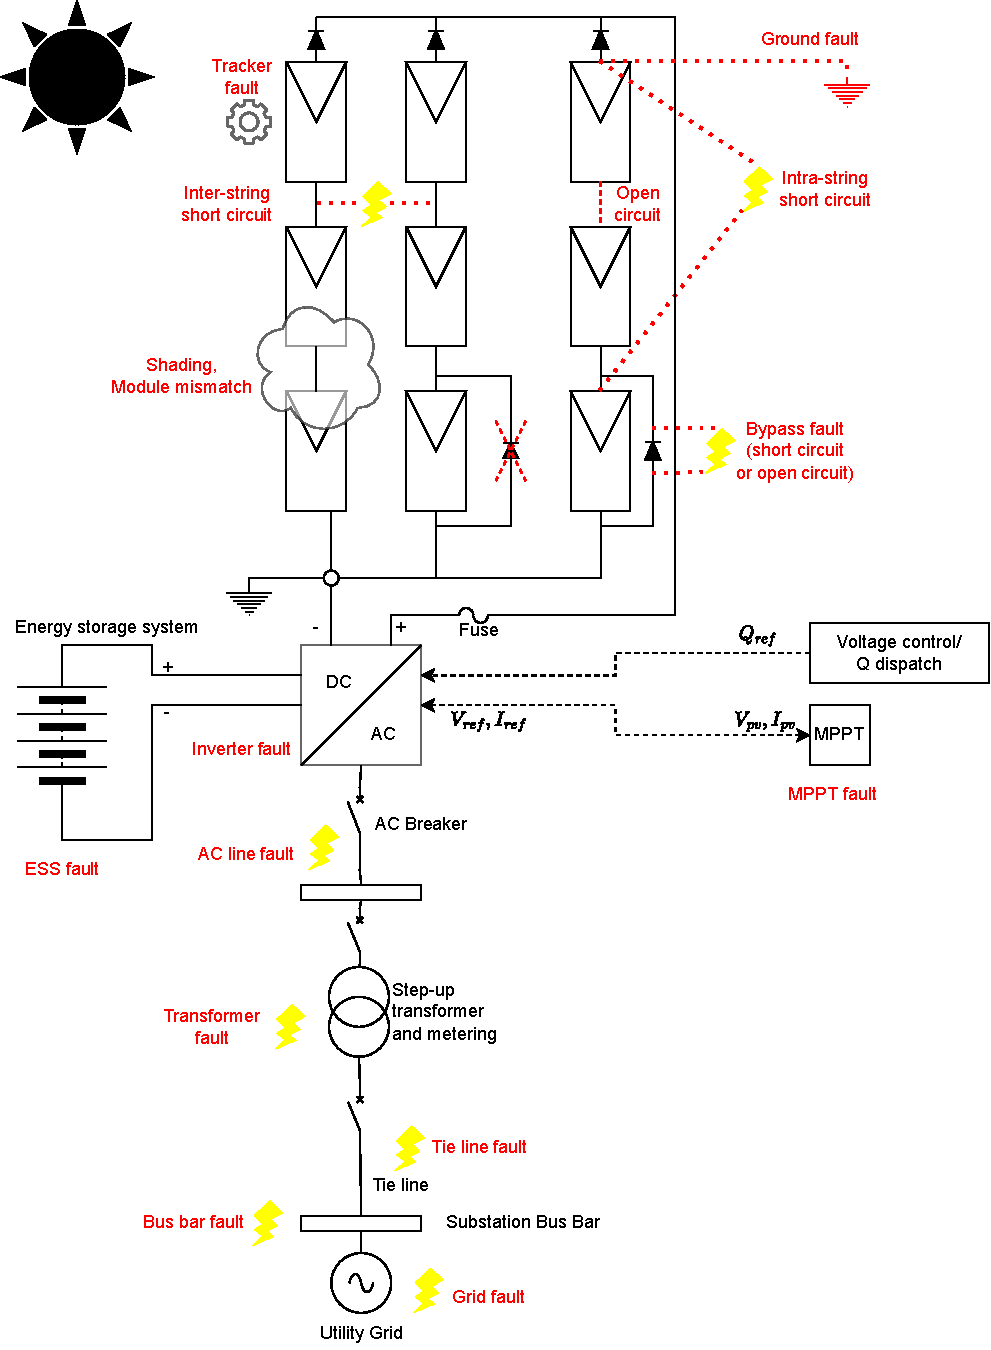
\includegraphics[width=15cm]{figures/chapter2/pvplant.drawio.pdf}
    \caption{Representation of utility-scale PV plant components and some possible faults.}
    \label{fig:topologies}
\end{figure}

Figure \ref{fig:topologies} presents a typical utility-scale PV plant architecture using the central inverter (or possibly multi-string inverter) configuration. Noticeably, many system components may fail in one or more ways, so monitoring and fault detection algorithms are essential to maintain state estimation. The main subsystems considered for anomaly detection are the following:

\begin{itemize}
    \item Solar photovoltaic panels (with or without bypass diodes).
    \item Tracking mount.
    \item Electrical cabling.
    \item Inverter(s) (mostly with Max Power Point Trackers).
    \item AC Transformer(s).
    \item Protection components (circuit breakers, fuses, surge protectors,
    etc.)
\end{itemize}

Most of these components have intrinsic variables, such as voltage and current values, that can help determine their operation states. Given that the utility grids (and the associated electricity market) integrate large-scale PV assets, some of the before-mentioned components require constant monitoring and control, achieved with adequate embedded systems and sensor infrastructure \cite{AIPV}. Since monitoring utility-scale PV assets relies on the investment and technologies employed, engineers must consider data availability when developing data-driven algorithms. Thanks to the continuous advancements in communication technologies, namely in IoT (Internet Of Things), data acquisition is becoming faster, more reliable, and more precise. Not only is this fundamental for real-time asset assessment, but it also allows better training of fault detection algorithms. However, on the industrial scale (in the order of MWp production), having sensors embedded in every PV module comes with a high economic cost. Inverters are the components that usually possess monitoring capabilities, though the grid-tie connection should also employ sensors. Consequently, these are the primary sources of information on utility-scale PV plants, with the most accurate, fast, and reliable data acquisition.

\begin{figure}[h!]
    \centering
    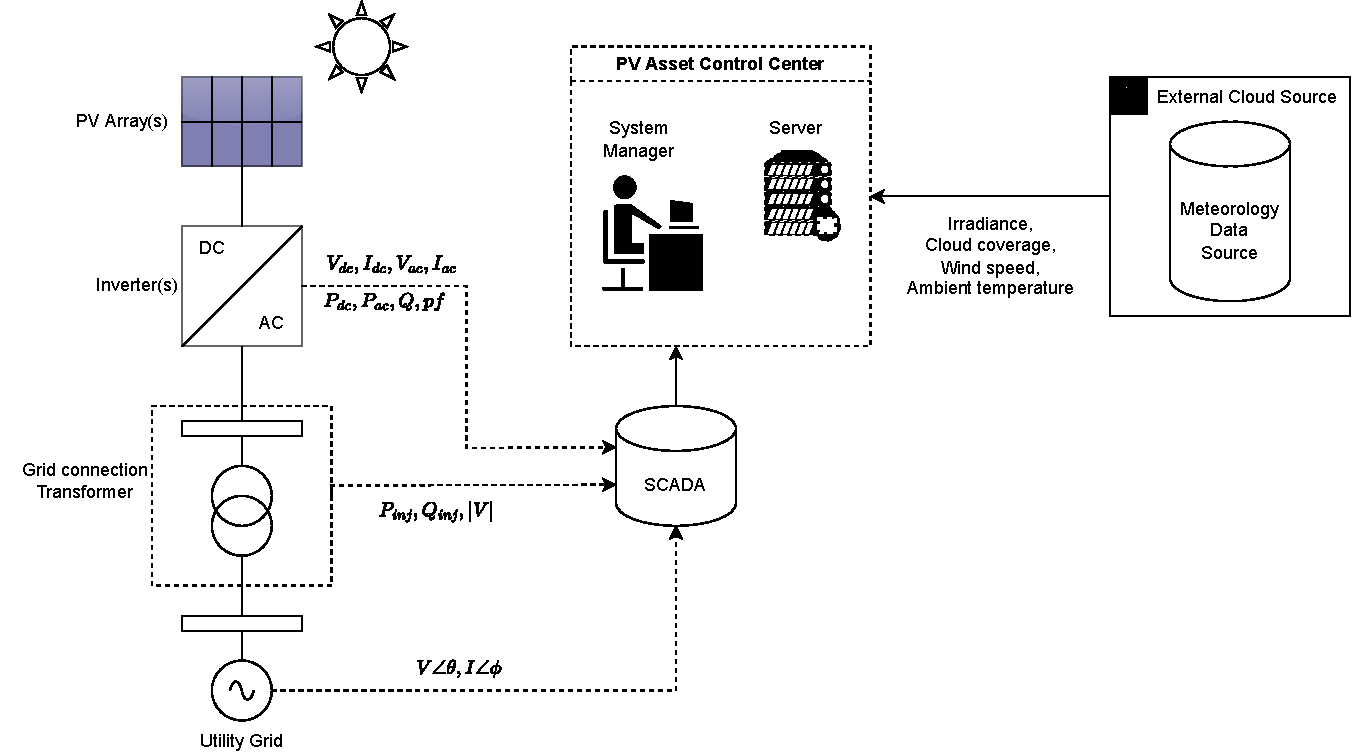
\includegraphics[width=\linewidth]{figures/chapter2/pvdata.drawio.pdf}
    \caption{Typical data flow of utility-scale PV power plants.}
    \label{fig:pvdataflow}
\end{figure}

Figure \ref{fig:pvdataflow} represents a simplified data flow representation of a grid-tied PV system's most commonly available state variables, with most of them suggested by the IEC 61724 standard \cite{iec61724}. An external meteorological data source is defined since the PV system manager usually needs climate information for (at least) forecasting purposes. The typical ranges of data acquisition periods in utility-scale PV assets are within 10 to 60 minutes.


\section{Faults in Photovoltaic Systems}

Several types of faults can occur in utility-scale photovoltaic (PV) power plants, which impact the performance and reliability of the system negatively. Unfortunately, some are very challenging to detect and protect the electrical installation against, thus requiring sophisticated detection algorithms \cite{Pillai2018}. Besides the economical price, their occurrence may even cause safety hazards, such as fires \cite{Alam2015}, thus the urgency in detecting or preventing such events early.

According to \cite{Pillai2018}, these faults can fit into three categories: electrical, mechanical, and environmental. Electrical malfunctions include short circuits, open circuits, and inverter failure, affecting the PV panels' power output and the system's overall efficiency. Mechanical faults include broken panels, damaged cables, and defective inverters, which can lead to system downtime and reduced performance (although not mentioned, solar tracker failures could also belong in this category). Environmental faults include extreme weather events, such as hail or strong winds, which can damage the PV panels and other components \cite{faults}.

The authors in \cite{Hong2022} cover a comprehensive review of most types of faults studied in the ambit of detection and classification algorithms. However, authors in \cite{Livera2019} have a more succinct fault categorization that better fits this work's scope. They categorize all the major PV system faults into either DC-side or AC-side. Figure \ref{fig:faults} represents this detailed categorization with a tree-like structure.

Although also prone to failure, most literature on fault detection and classification for photovoltaic systems does not encompass solar tracking faults: most studies cover fixed PV systems. The supervision and assessment of these subsystems' correct functioning can be sensor-based \cite{Stepanov2014} or image-based. Some authors developed fault detection methods for these apparatuses \cite{Amaral2021}, using image processing on aerial photography to determine modules' slopes. This category of failures should be better supported when developing electrical data-driven algorithms since they can significantly affect the system's efficiency.

\begin{figure}[h!]
    \centering
    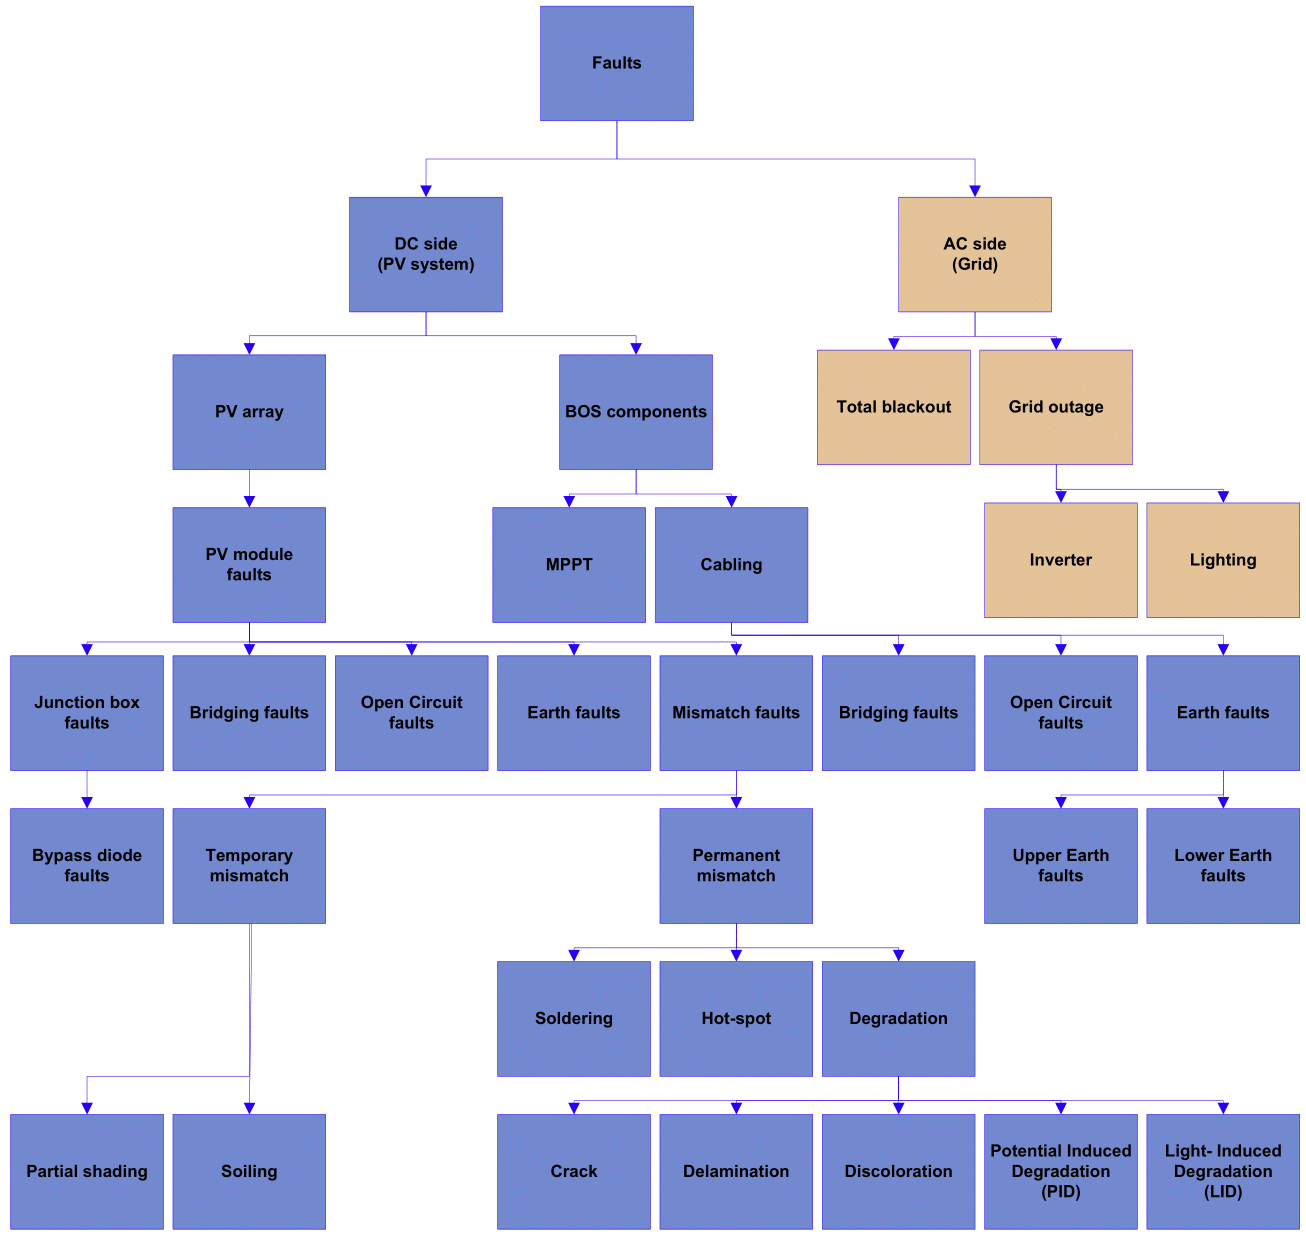
\includegraphics[width=14cm]{figures/chapter2/faults.png} \caption{"Failures in grid-connected PV systems."} Image source and copyright: \cite{Pillai2018}.
    \label{fig:faults}
\end{figure}

Throughout the literature \cite{Braun2011}, some of the most noted faults in the context of fault detection are:

\begin{itemize}
    \item Shading: partial coverage of a PV array or module, temporary or not. It might result in a Hot Spot fault.
    \item Soiling: dirt accumulation, blocking sunlight from reaching PV Cells. It might also result in a Hot Spot fault.
    \item Short circuit: either line-line or line-ground.
    \item Open circuit: connection breakage between modules.
    \item DC arc fault: electricity plasma arc formed on broken connections.
\end{itemize}

According to a 2017 survey conducted on five utility-scale PV plants in Italy \cite{Grimaccia2017}, the authors observed failure rates from <1\% to 3\% in the majority of plants and 81.8\% in the worst scenario. The high failure rate of the latter had a demonstrated cause that originated from manufacturing mistakes: snail trails. Besides this phenomenon, hot spot faults and bypass diode faults/disconnections were among the most common.

Alongside manufacturing failures, installation, planning, and other external effects can be the root cause for many of the presented faults \cite{sunny}.

\begin{figure}[h]
    \centering
    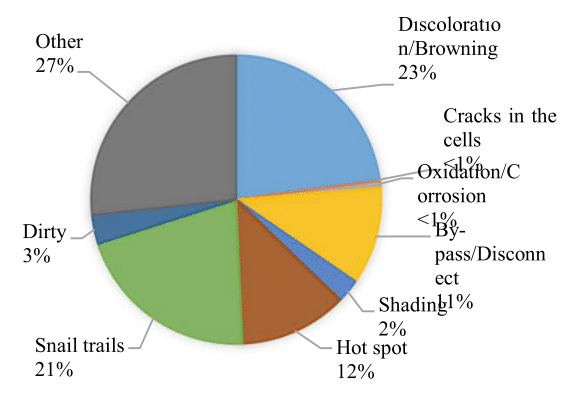
\includegraphics[width=8cm]{figures/chapter2/chartfailsurvey.png} \caption{"Circle chart related to the module defects in the 5 plants (over the total number of failures)."} Image source and copyright: \cite{Grimaccia2017}.
    \label{fig:faultchart}
\end{figure}

Having the distribution of fault types from real-life scenarios is quite helpful for formulating fault detection algorithms. It allows for better generation/selection of training data and class decisions. In figure \ref{fig:faultchart}, it is possible to observe the failure type distribution for 24.254 inspected modules. Soiling, shading, and mechanically related failures were not as prominent, with only a group share of around 6\%. It is relevant to note that discoloration represents almost a quarter of all faults.

Although the study had a limited geographic scope, with only a few power plants diagnosed, it allows for a more realistic view of the common scenarios encountered in typical operational ground-mounted utility-scale PV power plants.

Due to the difficulty of classifying some of these faults, given their similarity on the consequent effect in the system, it will be seen in further sections that most fault detection algorithms only endeavor to classify between two to five types of reviewed faults.

\section{Modeling photovoltaic's physical/electrical behavior}

Photovoltaic cells are the fundamental components of photovoltaic panels. They are made from semiconductor materials like silicon and absorb photons that generate electric current. Their electrical behavior is characterizable using the current-voltage (I-V) equation \ref{eq:iv}. This equation, which represents a fundamental relationship governing the operation of PV cells, can be used to predict their performance under various operating conditions, such as differing solar irradiance and temperatures.

\begin{equation} \label{eq:iv}
    I = I_{ph} - I_d \times (e^{\frac{q \times (V_{pv} + I_{pv} \times R_{s})}{n \times k \times T}} - 1) - \frac{V_{pv} + I_{pv} \times R_s}{R_p}
\end{equation}

$I_{ph}$ (A) is the light-generated current;
$I_{0}$ (A) is the reverse saturation current;
$V_{pv}$ is the module's terminal voltage;
$I_{pv}$ is the module's output current;
$R_{s}$ ($\Omega$) is the series resistance;
$R_{p}$ ($\Omega$) is the shunt resistance;
$n$ (adimensional) is the diode ideality factor;
$k$ (J/K) is the Boltzman constant;
$T$ (K) is the cell temperature;
$q$ (C) is the electron charge;

For state estimation, it is crucial to accurately model PV modules' performance from the DC side of power converters. This information is vital for designing and optimizing PV power systems, as it enables predicting PV module performance under different conditions, as mentioned before. Accurate PV models are also essential for state estimation and fault detection, as they provide critical information about their health and performance, allowing for early identification of potential issues. Moreover, they can be used to optimize the control and operation of PV power systems, improving their efficiency and reliability \cite{Braun2011}.

Physical and empirical models broadly categorize the several state-of-the-art methods for modeling photovoltaic modules \cite{Braun2011}. Physical models lie on the fundamental physical principles governing PV modules' operation. They typically require detailed knowledge of the PV module's electrical and optical properties, such as its current-voltage (I-V) characteristics, spectral response, and temperature dependence. These models can accurately predict the PV module's performance under a wide range of operating conditions, but they may be complex and computationally intensive to implement \cite{Kumar2019}. On the other hand, empirical models are based on experimental data and are typically more straightforward to implement. However, they may not be as accurate as physical models, especially under conditions that differ significantly from those used to generate the experimental data (usually STC) \cite{Braun2011}. Some examples of state-of-the-art physical models for PV modules include the single-diode model (the five-parameter model) and the two-diode model \cite{Godina2017}. In contrast, one of the most used state-of-the-art empirical models is the Sandia model \cite{Braun2011}. The choice of modeling method will depend on the specific application and the required level of accuracy and complexity; in some cases, there can be a combination of physical and empirical models.

In the case of utility-scale PV systems, detailed knowledge of the module's electrical and optical properties of empirical data may be limited, and building a model is only possible by recurring to datasheet information. A complex model that requires more detailed information may not be feasible in such cases, and a simpler model that relies on fewer input parameters is more appropriate. Given the excellent trade-off between complexity and accuracy, the single-diode model suits this use case.

\subsection{The five-parameter model}

Figure \ref{fig:onediodedraw} presents the single-diode model representation of the photovoltaic module. According to the five-parameter model, the unknown parameters are determined by fitting the model to experimental data or using data from the PV module's datasheet. The single-diode model can predict the PV module's performance under various operating conditions while maintaining reasonable accuracy. However, remembering that the single-diode model is a simplified representation of the PV module, it will have poor accuracy under certain situations compared to the more representative two-diode model \cite{Godina2017}.

\begin{figure}[H]
    \centering
    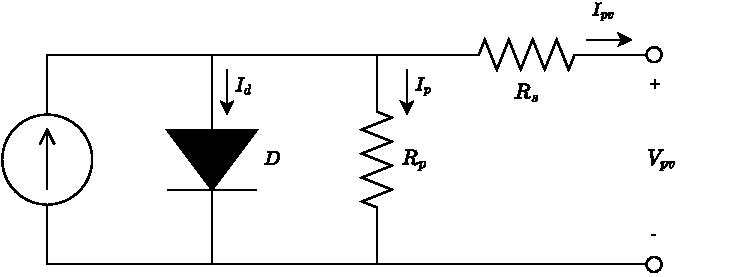
\includegraphics[width=10cm]{figures/chapter2/onediode.drawio.pdf} \caption{Single-diode model for photovoltaic modules.}
    \label{fig:onediodedraw}
\end{figure}

% \section{Characteristics of Photovoltaic Faults}
% ! fazer isto ou não?
% To better understand the effect of faults in photovoltaic systems, we review 

\section{Literature on Fault Detection and Classification for Photovoltaic Systems}

The parent field of fault detection is anomaly detection (also known as outlier detection), a highly studied subject in the scope of statistics \cite{Prasad2009}, applied in many scientific areas. Classification is also well-studied in this field, with applications in numerous scientific contexts, from medical diagnosis to airport safety \cite{classification}. Consequently, adaptations of generic tools and ad hoc methodologies have originated to aid in solving fault detection and classification problems in photovoltaics.

According to \cite{AIPV}, the tools dedicated to PV fault detection and state estimation mostly come from mathematical/statistical methodologies, machine learning, and deep learning applications. Regarding the three general problem-solving principles mentioned before, machine learning and deep learning are the most popular and successful ones for recent applications that ought to solve complex problems. However, this categorization needs to be revised, with contemporary literature suggesting many developed methodologies from different backgrounds, thoroughly reviewed in \cite{Hong2022} and \cite{Livera2019}. In \cite{Hong2022}, the authors consider two principal fault detection and classification algorithm branches: image-based and electrical-based, while \cite{Livera2019} also distinguishes numerical-based techniques. Image-based refers to aerial or visual capture of the PV array by photography and thermal imaging, commonly used along with artificial intelligence algorithms for assessing the photovoltaic module's physical state. Although the contribution and importance of such methods are appreciable, this work will mainly focus on the electrical-based and numerical-based ones, as the use case of the developed tool is bound to this type of data.

Categorizing methodologies becomes fuzzy, considering that some literature mixes physical behavior models with machine learning, statistics, and signal processing. Figure \ref{fig:techniques} is an attempt to present a structure inspired by the review made by \cite{Hong2022}, \cite{Livera2019}, and this work, with a focus on the techniques more relevant for our scope. Hybrid models are ubiquitous since combining robust statistical, signal processing, ML, or DL models and PV's electrical characterization can achieve more remarkable results. Accordingly, a better representation than figure \ref{fig:techniques} would be an incomprehensible mesh of connections representing the permutations between category aggregation.
 
\begin{figure}[h]
    \centering
    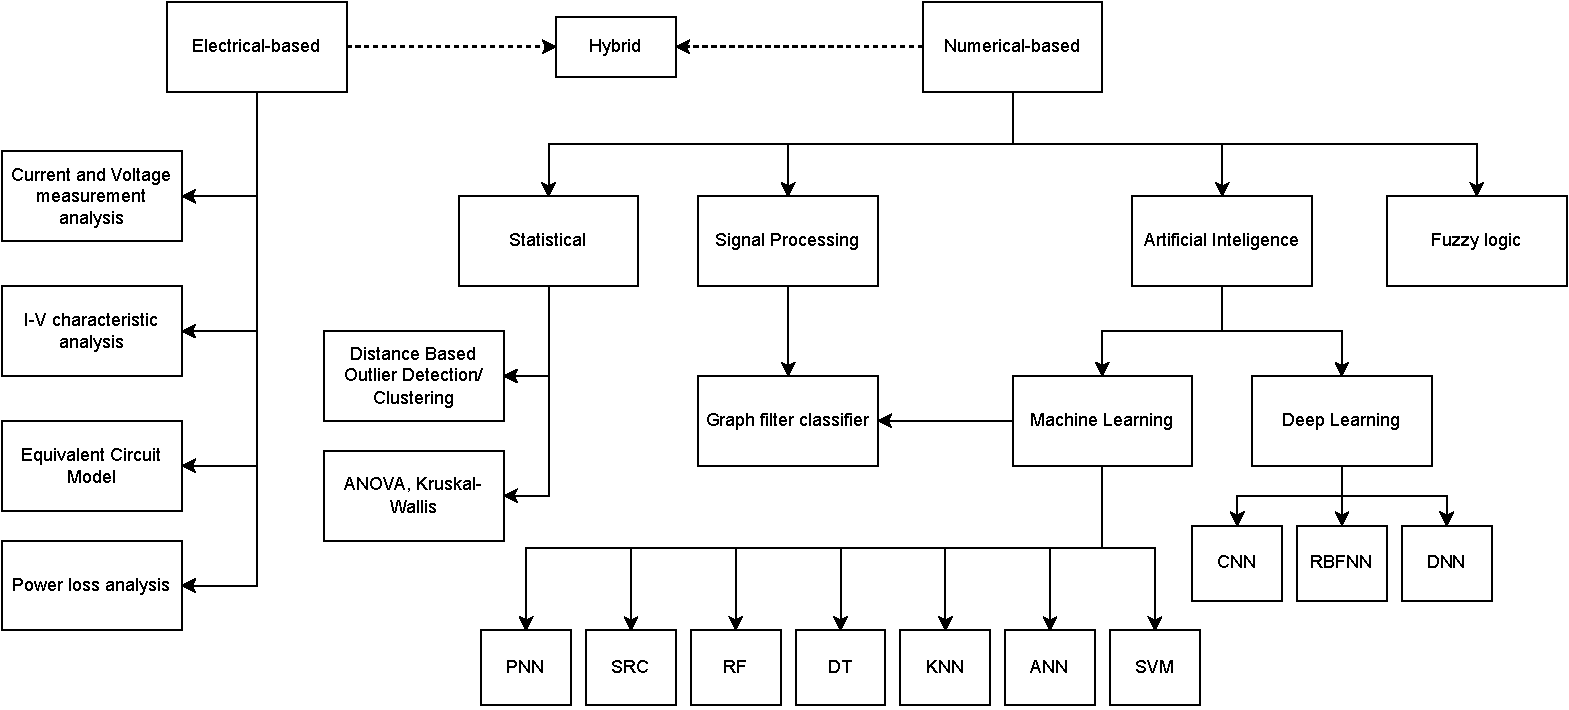
\includegraphics[width=15cm]{figures/chapter2/techniques.drawio.pdf} \caption{Representation of some of the methodologies employed in fault detection for PV systems.}
    \label{fig:techniques}
\end{figure}

Deciding which methodologies to revise is necessary to avoid wandering in the literature. The developed tool in this work must meet certain real-life constraints, such as data availability, frequency, accuracy, PV system configuration, and context. Therefore, we consider each methodology's potential (qualitative) as the proposed algorithms' adaptability to the same expected restrictions. This evaluation process confines the methodology review to emphasize the ones thought to be most capable of implementation in a real scenario. Therefore, the following sections will not cover an extensive literature review; we do not intend to repeat the works of \cite{Hong2022} and \cite{Livera2019}, only presenting interesting or adequate methodologies related to this work's scope.

\subsection{Statistical and Signal Processing Algorithms}

Statistical methodologies look into historical data to find the characteristics of how samples relate to the population (interpolation). These methodologies yield good results in case studies of PV farms that have been logging data for a considerable time, suffering in the cases that do not. Therefore, they are limited in that it is required to have curated data sets of historical significance for relevant features of the studied systems.

The literature on fault detection algorithms based on statistical and signal processing is mostly quite dated (\cite{Buddha2012}, \cite{Zhao2014}, \cite{Vergura2008}), given that more recent machine learning methods have become increasingly attractive in this matter. Nonetheless, anomaly (or outlier) detection statistical algorithms can be used for fault detection in PV systems by identifying unusual patterns or deviations from normal behavior in the data collected from the PV system. Distance-based methods may be adequate, such as the Euclidean, Mahalanobis, and MCD-based distances \cite{Braun2011}. Although simple, these techniques might only work for detecting outliers in the context of PV systems if they are scale-invariant (due to the different magnitude in the system's state variables) and resilient to outlier contamination (which only MCD-based distance is capable of). In \cite{Vergura2008}, the authors applied Analysis of Variance (ANOVA) and Kruskal-Wallis test for inverter failure detection, with the only downside of only being able to identify outliers in a sub-array resolution, i.e., not for specific string or module failures.

Some algorithms consider incoming data from PV systems as signals, allowing the adaptation of signal processing theory to develop ad hoc algorithms. Coming up with a relatively simple algorithm, the authors in \cite{Iles2021} propose a power-based fault detection method that only requires delayed samples of the PV array's power output and a threshold. It reasons that since the power output of PV systems cannot vary beyond a given point, considering a very short-term period (milliseconds), significant perturbations in this variable can be associated with faults. Although the simplicity and ease of implementation, it is clear that the success of this method requires feeding the algorithm with relatively high-frequency data, which would only be feasible on-site (and with specialized monitoring equipment).

In \cite{Fan2020}, the authors successfully formulated a graph signal processing algorithm for fault classification that yields increasingly better results when there is a considerable amount of labeled data, although its training is only semi-supervised. The results outperformed other standard machine learning methods for the same training data, given 30\% or more of labeled data. On another note, the data utilized came from the PVWatts \cite{Dobos2013} dataset, and the PV system is on a small scale (ASU testing facility \cite{Rao2016}) possessing a monitoring density and capability that can be considered irrealistic for utility-scale. This same data source is present in many other reviewed works.

The authors in \cite{Katoch2018} displayed another excellent use for graph theory, although not specifically for fault detection: they implemented a consensus-based distributed approach to minimize the impact of noise in acquired data from the PV array. By formulating a data propagation algorithm that resulted in measurement convergence, they achieved higher accuracy for state estimation.

With both graph theory-based algorithm proposals, this field sparks interest in its usage for the upcoming formulated methodology, given that it would be desirable to achieve an algorithm that features fault detection alongside data consensus.


\subsection{Machine Learning Algorithms} \label{subsec:machinelearning}

Machine learning is the trending way of solving increasingly complex and nonlinear problems, as neural networks (or other learning structures) can better model complex, non-trivial, and nonlinear relations between data. Still, they are as good as the training data, with many designs requiring a lot of representative learning examples to achieve good results. Their output can also be very obfuscated (depending on the technique), meaning that many methods do not allow a direct interpretation of the relationship between inputs and outputs. This "black-box" characteristic, specifically of neural networks, is considered a disadvantage. Besides, extrapolating data remains a challenge when classically using these structures. Still, they have immense applications for PV systems, from MPP (Max Power Point) estimation to power forecasting, soiling, and fault prediction.

In \cite{Kumari2022}, the authors utilize an ANN to classify short circuit and hot spot faults. This algorithm achieved an outstanding 98.4\% classification accuracy, yet the data originated from \textit{MatLab/Simulink} simulations and only considered two classes of faults. Because the inputs were the variation of voltage and current ($\frac{dV}{dt},\frac{dI}{dt}$), the algorithm required data sampling with relatively high frequency (>5Hz). This work will not regard such methodologies as background for the upcoming tool since requiring high-frequency simulated data while covering only two fault types is quite far from a real utility-scale PV system scenario.

The trend of utilizing simulated data (sometimes without even added noise) has been a target of criticism in \cite{Aziz2020}. Accordingly, this work also emphasizes that the literature shows many proposed ML (and other types of) techniques that fall into this concept, which makes selecting appropriate methodologies to base future work on a challenging task.

The proposed ANN solution in \cite{Rao2019} is remarkable by the diversity of fault classification achieved: STC, short circuit, varying temperature, partial shading, complete shading, degraded modules, ground fault, and arc fault. It presents one of the most accurate fault class coverage in the group of literature that utilizes synthetic noiseless data. Hence, the cyber-physical conceptualization and data preprocessing (clustering) demonstrated can be admired, but not forgetting that validation data came from a relatively unrealistic setting. 

In \cite{Rao2021}, there is a captivating proposal of utilizing an autoencoder and pruned neural network to separate the tasks of detecting and classifying faults, which resulted in one of the most performant ML approaches in the literature. The algorithm classifies five states: degraded, shaded, soiled, short circuit, and STC, utilizing nine inputs representing voltage, current, power, and irradiance available from the MPPT, datasheet, or meteorological sources. While the neural network pruning adds complexity, it resulted in a better generalized and lighter-weight trained model suitable for faster detection times. Even though using data from a small-scale PV system, the presented algorithm and its assumptions may make it possible to adapt and implement in an industrial scenario.

Regarding performance, the work in \cite{Kilic2020} proposes a sparse representation classifier (SRC) that evaluates if the system has line-to-line or line-to-ground faults for varying operating conditions. Although a drop in accuracy occurred for extreme circumstances, it is impressive that the algorithm identifies faults in such varied operating conditions: 10 to 50 degrees ambient temperature, 200 to 1000 $W/m^2$ irradiance, 10 to 60 \% of mismatch, and 0 to 25 $\Omega$ of fault resistance. The feature extraction step was also very impressive, which could be a determining factor in the method's performance. Unfortunately, this work also does not validate results with experimental data and only uses simulation as a source. However, the demonstrated computational performance, both in terms of training cost and utilization speed, its usage without the need for training for parameter tuning, the straightforward implementation, and consistent convergence, suggests the potential for this alternative in the face of other ML methodologies. The authors also emphasize that sparse representation might be utilized alongside different learning algorithms for classification, opening the door to many possible future implementations.

Authors in \cite{Uehara2021} made an exciting yet far-fetched proposal, developing a quantum neural network (QNN) for PV fault classification. They trained the QNN to predict only two scenarios: faulty or standard, but required up to four training days, resulting in 93.89\% accuracy. For comparison, the classical ANN took twenty seconds to train and achieved 95.39\% accuracy. Although the methodology showcases the potential of quantum computing for this field, its preliminary results still distance itself from the traditional methods.

An abundance of ML methods has been tested and reviewed in this field (\cite{Hong2022},\cite{Livera2019}), utilizing structures such as SVM, KNN, and RF. Nonetheless, the results of \cite{Rao2021}-\cite{Kilic2020} sparked the most interest in this work's scope.

\subsection{Deep Learning Algorithms}

Deep learning is a branch of machine learning, with the term "deep" referring to amplified machine learning structures that ought to understand data patterns through more complex and intertwined artificial neuron connections. A simple example of a deep learning model would be the design of an artificial neural network with multiple hidden layers (DNN), with the intuition that each of these "extra" layers achieves feature/pattern recognition in a cascade. Other DL structures include the LSTM, CNN, and RBFNN. They have been explored alongside classical machine learning techniques for PV fault detection, although the known disadvantage is a usually high computational cost and relatively tricky implementation. The typical application of these techniques is in image-based solutions \cite{termoreview} since they require classification based on 2D data from various image acquisition equipment \cite{termo}, \cite{dlpv}. Given the 1D characteristic of raw electrical data, little literature considers these techniques for fault detection, as it implies an extra step of increasing dimensionality. However, there are some promising results in doing so \cite{Aziz2020}.

In \cite{Aziz2020}, not only is a DL technique presented for fault detection and classification, but there is also the best attempt at comparative evaluation against other methodologies. As mentioned, much of the literature presents results solely based on particular datasets comprising simulated noiseless data, invalidating any significant quantitative comparison.

Authors in \cite{Krizhevsky2012} use a CNN model based on the pre-trained AlexNet for classification and feature extraction, allied with a classical ML model also for classification. The classified faults were arc fault, partial shading, open circuit, and short circuit. While the experiments utilized simulation data, adding noise and an abundance of heterogenous operating conditions better resembled a real scenario. Considering the same noisy data, other tested methodologies present 22-70\% average accuracies, with the proposed fine-tuned AlexNet CNN reaching a maximum of 70.45\%. This work presents one of the best benchmarks in the literature, with decent coverage of other state-of-the-art ML and DL algorithms, while demonstrating the most realistic results and a sophisticated methodology proposal.

\subsection{Proposed method's scope}

While classical fault detection resides in the synchronous and direct evaluation of state and climate variables, realistic industrial scenarios can have data from various types, sources, and acquisition rates.
It is also important to realize that monitoring equipment can register erroneous information, and current communication technology is also susceptible to delays and data loss.
To reflect all the issues of tangible PV assets with kW to MW of power, the authors in \cite{Livera2022} made excellent failure diagnosis and loss estimation algorithms tailored for industrial-scale PV farms. In such work, it is noticeable how different the algorithms are from classical, less "practical" approaches. Their approach inspires this work to stray from standard practices and formulate another methodology with the same orientation for practical implementation in large-scale PV.
Recent developments in the intelligent composition of deep learning structures aligned with graph theory spark some interest in their application to this field, such as the new deep learning technique named Cell Complex Neural Networks \cite{Hajij2020}. The motivation for choosing such a structure comes from its data propagation and consensus capability. The propagation techniques utilized in a CXN appeal to graph theory, dividing a system into other subsystems and components (nodes, also called cells in \cite{Hajij2020}) that share information. Even if the direct application of this structure might not be feasible or grant better results in the context of fault detection, its modification to meet the scope's needs could result in a robust and efficient solution. It serves as another source of inspiration for this work.

According to the reviewed methodologies, the proposed tool will pertain to the hybrid category since, while having a central component of fuzzy logic, it may also require some modeling of the PV system to extract more results. In reality, it is relatively challenging to categorize. It aims at an asynchronous and online application, which differs from most current methods. It desires to bring a comprehensive benchmark utilizing a dataset with samples from tangible utility-scale PV assets, allowing its assessment in a realistic scenario.

\begin{table}[h]
    \centering
    \caption{Comparison of literature that inspired this work.}
    \label{tab:comparelit}
    \resizebox{\textwidth}{!}{%
    \begin{tabular}{|l|l|l|l|l|c|c|l|l|}
    \hline
    \multicolumn{1}{|c|}{\textbf{\begin{tabular}[c]{@{}c@{}}Reference\\ and year\end{tabular}}} &
      \multicolumn{1}{c|}{\textbf{\begin{tabular}[c]{@{}c@{}}Data\\ Source\end{tabular}}} &
      \multicolumn{1}{c|}{\textbf{Inputs}} &
      \multicolumn{1}{c|}{\textbf{\begin{tabular}[c]{@{}c@{}}Proposed\\ methodology\end{tabular}}} &
      \multicolumn{1}{c|}{\textbf{\begin{tabular}[c]{@{}c@{}}Classified Faults\\ (alongside STC)\end{tabular}}} &
      \textbf{\begin{tabular}[c]{@{}c@{}}Validation\\ data\\ realism\end{tabular}} &
      \textbf{\begin{tabular}[c]{@{}c@{}}Computational\\ cost\end{tabular}} &
      \multicolumn{1}{c|}{\textbf{Notes}} &
      \multicolumn{1}{c|}{\textbf{Drawbacks}} \\ \hline
    \begin{tabular}[c]{@{}l@{}}\cite{Aziz2020}\\ \\ 2020\end{tabular} &
      \begin{tabular}[c]{@{}l@{}}Simulated \\ PV System,\\ added noise\end{tabular} &
      \begin{tabular}[c]{@{}l@{}}Irradiance,\\ Temperature,\\ Short circuit current,\\ Open circuit voltage,\\ PV current,\\ MPP current,\\ MPP voltage,\\ MPP power.\\ Boost converter\\ Maximum current,\\ Voltage and power.\end{tabular} &
      \begin{tabular}[c]{@{}l@{}}Pre-trained\\ CNN (AlexNet)\\ for feature extraction\\ and classification\end{tabular} &
      \begin{tabular}[c]{@{}l@{}}Arc fault,\\ Partial shading,\\ Fault\\ during\\ partial shading,\\ Open circuit, \\ Line to line SC\end{tabular} &
      Moderate &
      High &
      \begin{tabular}[c]{@{}l@{}}Resilient against noisy data.\\ Outperforms classical ML\\ methodologies.\end{tabular} &
      \begin{tabular}[c]{@{}l@{}}Requires data samples\\ from the MPPT\\ boost converter.\end{tabular} \\ \hline
    \begin{tabular}[c]{@{}l@{}}\cite{Kilic2020}\\ \\ 2020\end{tabular} &
      \begin{tabular}[c]{@{}l@{}}Simulated\\ PV System,\\ no added noise\end{tabular} &
      \begin{tabular}[c]{@{}l@{}}MPP voltage, \\ MPP current,\\ Short circuit current,\\ Open circuit voltage,\\ Irradiance\end{tabular} &
      \begin{tabular}[c]{@{}l@{}}Sparse\\ representation\\ classifier\end{tabular} &
      \begin{tabular}[c]{@{}l@{}}Line to line SC\\ Line to ground SC\end{tabular} &
      Low &
      Low &
      \begin{tabular}[c]{@{}l@{}}Very fast learning speed compared to\\ classical ML structures.\\ Straightforward implementation.\\ Good feature extraction process.\end{tabular} &
      \begin{tabular}[c]{@{}l@{}}Validation data\\ was very idealistic.\\ Only classifies line to line\\ and line to ground faults.\end{tabular} \\ \hline
    \begin{tabular}[c]{@{}l@{}}\cite{Fan2020}\\ \\ 2020\end{tabular} &
      \multirow{2}{*}{\begin{tabular}[c]{@{}l@{}}PVWatts\\ dataset\end{tabular}} &
      \multirow{2}{*}{\begin{tabular}[c]{@{}l@{}}MPP voltage,\\ MPP current,\\ Short circuit current,\\ Open circuit voltage,\\ Irradiance, Fill factor,\\ Temperature,\\ Gamma ratio,\\ Maximum power\end{tabular}} &
      Graph signal processing &
      \multirow{2}{*}{\begin{tabular}[c]{@{}l@{}}Shading\\ Degraded modules\\ Soiling\\ Short circuit\end{tabular}} &
      \multirow{2}{*}{High} &
      Low &
      \begin{tabular}[c]{@{}l@{}}Semi-supervised,\\ allows usage of\\ unlabeled data for training.\\ Better accuracy relatively to other\\ ML methods for less labeled data. \\ Low training cost.\end{tabular} &
      - \\ \cline{1-1} \cline{4-4} \cline{7-9} 
    \begin{tabular}[c]{@{}l@{}}\cite{Rao2021}\\ \\ 2021\end{tabular} &
       &
       &
      \begin{tabular}[c]{@{}l@{}}Autoencoder for detection\\ and pruned neural network\\ for classification\end{tabular} &
       &
       &
      Medium &
      \begin{tabular}[c]{@{}l@{}}Separate the task of\\ detection from classification,\\ allowing for other combinations.\\ Good performance method\\ considering the\\ algorithms complexity.\\ Pruning creates an\\ ANN less prone to overfitting.\end{tabular} &
      \begin{tabular}[c]{@{}l@{}}Requires more complex\\ training phase, for two\\ different networks, and\\ utilizing a dropout\\ algorithm for pruning.\end{tabular} \\ \hline
    \end{tabular}%
    }
    \end{table}

Table \ref{tab:comparelit} represents a summary that compares four of the most inspiring reviewed proposals.
\chapter{Preliminary Work Plan} \label{chap:chap3}

% TODO

\chapter{Conclusions}

% TODO
\chapter{CellTAN: Cellular Time Activation Networks} \label{chap:chap4}

Distributed information systems characterized by time series data present various challenges, primarily due to their complex and dynamic nature. The sheer volume of data that must be processed and analyzed in real time is a significant challenge, leading to concerns over storage, computation, and scalability. Moreover, data quality issues such as missing or incomplete data and data heterogeneity arising from sourcing data from disparate sources with varying consistency and structure further exacerbate these challenges. Another critical challenge of these systems is handling the temporal aspects of time series data, requiring specialized pre-processing, feature extraction, and modeling techniques. The distributed nature of these systems further complexifies matters, with issues encompassing data synchronization and accuracy being a common concern. Furthermore, their implementation in real-world applications requires robust mechanisms for data security and privacy, which adds a layer of complexity to the design and implementation of these systems.

\begin{figure}[h!]
    \centering
    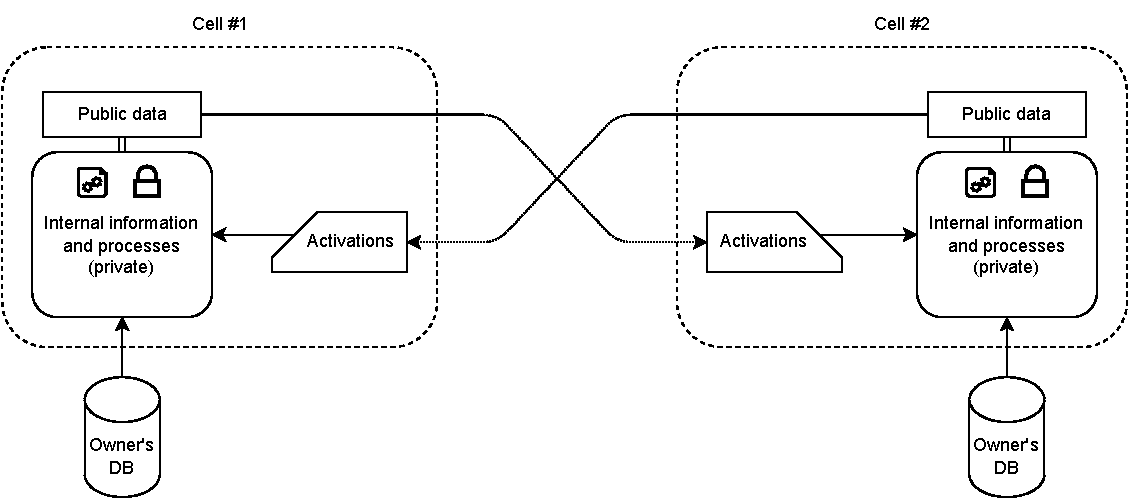
\includegraphics[width=12cm]{figures/chapter4/cell/intro.pdf}
    \caption{Simples CellTAN Network of two cells cooperating.}
    \label{fig:celltanintro}
\end{figure}

This chapter proposes a novel tool entitled CellTAN (Cellular Time Activation Network) that undertakes those challenges. CellTAN represents sparse yet interconnected components that function independently, cooperatively, and asynchronously. Inspired by other effective mechanisms like GNNs, CXNs, and Weighted Cross-Connection Networks (WCCNs), CellTAN uses a graph-like structure to represent a network of components with nodes and connections. Following the introductory chapters, its primary purpose is to detect abnormal scenarios on PV systems. However, its generalized formulation introduces other valuable features which come naturally from fulfilling this goal. Such are state estimation, forecasting, and capturing the value in data from different PV asset owners without violating their privacy. For briefness' sake, we will unfold details about its benefits during the rest of this chapter.

Instead of tackling fault detection and classification in a classical centralized manner, which is already extensively showcased throughout the literature, this tool approaches this problem with a paradigm change: a distributed and asynchronous data coherence system. By having a virtual representation closely related to the physical form of sparse systems, we can leverage the relationships between components to assess their correct (or incorrect) operation. While initially designed for photovoltaic (PV) systems, the concepts of cells, connections, neighbors, time series, and uncertainty are universal and applicable to other fields such as biology, physics, and more. Thus, the potential for generic applicability sparks the interest to not bake specifics of PV systems directly into this tool, allowing its usage for other subjects. Figure \ref{fig:celltanintro} represents a minimal scenario for a network: only two cells. It showcases some terms specific to this tool that might be difficult to grasp initially, such as trust, events, and activations. Consequently, the glossary in \ref{sec:glossary} and detailed explanations throughout this chapter serve to clarify them.

Vast and scattered information across multiple agents is a common scenario faced by the industry of AI for energy systems, which cannot be aggregated due to privacy and confidentiality reasons. Nevertheless, its conjunction could have a lot of added value, given the similarity of certain assets: PV plants (as well as wind farms) from different owners in neighboring geographical regions. This information-sharing potential for AI algorithms motivates the development of a mechanism that communicates information between differently owned assets without any of the compromises above. However, as stated before, data acquisition in PV scenarios is scarcely synchronous and might only occur in equal time resolutions for some of the different components. The CellTAN addresses these issues with an instrument called \textbf{Time activations}. It proposes a new way of communication that decouples from the needs of units, sampling rate, and synchronization, avoiding resampling, normalization, or even obfuscation (to protect privacy). This mechanism is a core feature of the tool since it will be the means that will allow connecting different stakeholders' data, and section \ref{sec:thecell} develops this matter thoroughly. Likewise, succeeding sections formulate the working of the \textbf{cell} and its interactions within the network. Since it is the core component, understanding its behavior is crucial for a complete understanding of the tool.

\section{Glossary} \label{sec:glossary}


\begin{itemize}
    \item \textbf{Knowledge base}: Refers to registered historical knowledge (samples) of time series variables.

    \item \textbf{Inputs}: Uniform fuzzy numbers (not necessarily, but it is the current choice) that represent one sample of the group of time series variables that define the state of a cell.

    \item \textbf{Outputs}: Similar to inputs, but obtained through some computations.

    \item \textbf{Time decay}: A process associated with increased uncertainty of variables over time.

    \item \textbf{Activations}: Timestamps of past occurrences on a knowledge base with a non-zero membership value against a set of recent inputs.

    \item \textbf{Events}: Occurrences that the cell reports back to the hub, usually triggered by exceeding parametrized thresholds.

    \item \textbf{trust}: A decimal number that represents how coherent two cells' activations are with each other. Besides its instantaneous computed value, it can also come from a cumulative computation on a defined time window.

    \item \textbf{hub}: The central component of the cell network, which facilitates its visualization, management, and expansion. It acts as the proxy agent between the cell's communication.

\end{itemize}

\section{The Cell} \label{sec:thecell}

% TODO falta mencionar que o dono da célula é que é responsável por estabelecer conexões

\subsection{Principles}

A cell is an independent entity composed of \textbf{data} and \textbf{processes}. The idea is to abstract fundamental system components (e.g., inverters, MPPTs) into this virtual entity. With an added intelligence layer and featuring a few different processes, it assesses its current state based on all available internal and external information, adding value to the existing data acquisition and monitoring systems. As an individual part of the system, it follows a set of rules that define its intrinsic and extrinsic behavior. These rules address data privacy, request boundaries, and real-world operational limitations.

\paragraph*{Independence} During operation, independence on neighbors or other network entities for continuous processing of outputs results in a more robust system and increases cell availability. Thus, given any connection cutoffs, the cell shall be unbothered by its surroundings and continue operating in an isolated state. Isolation is not preferred, but enduring it until outside contact is re-established avoids shutdown and startup procedures.

\paragraph*{Selfish Computations} The cell is selfish in that it will not perform any computations based on the request of others. This aspect creates a fundamental layer of protection against overloading the infrastructure in which it is deployed, which also increases availability.

\paragraph*{Data accessibility} Although selfish in computations, the cell shall provide access to select data valuable to the network. However, not all internal data is shared, and public data shall not compromise the cell's privacy (more on this later).

\subsection{Processes and Data}


The cell has a main process loop that executes a sequence of actions periodically: 

\begin{figure}[h!]
    \centering
    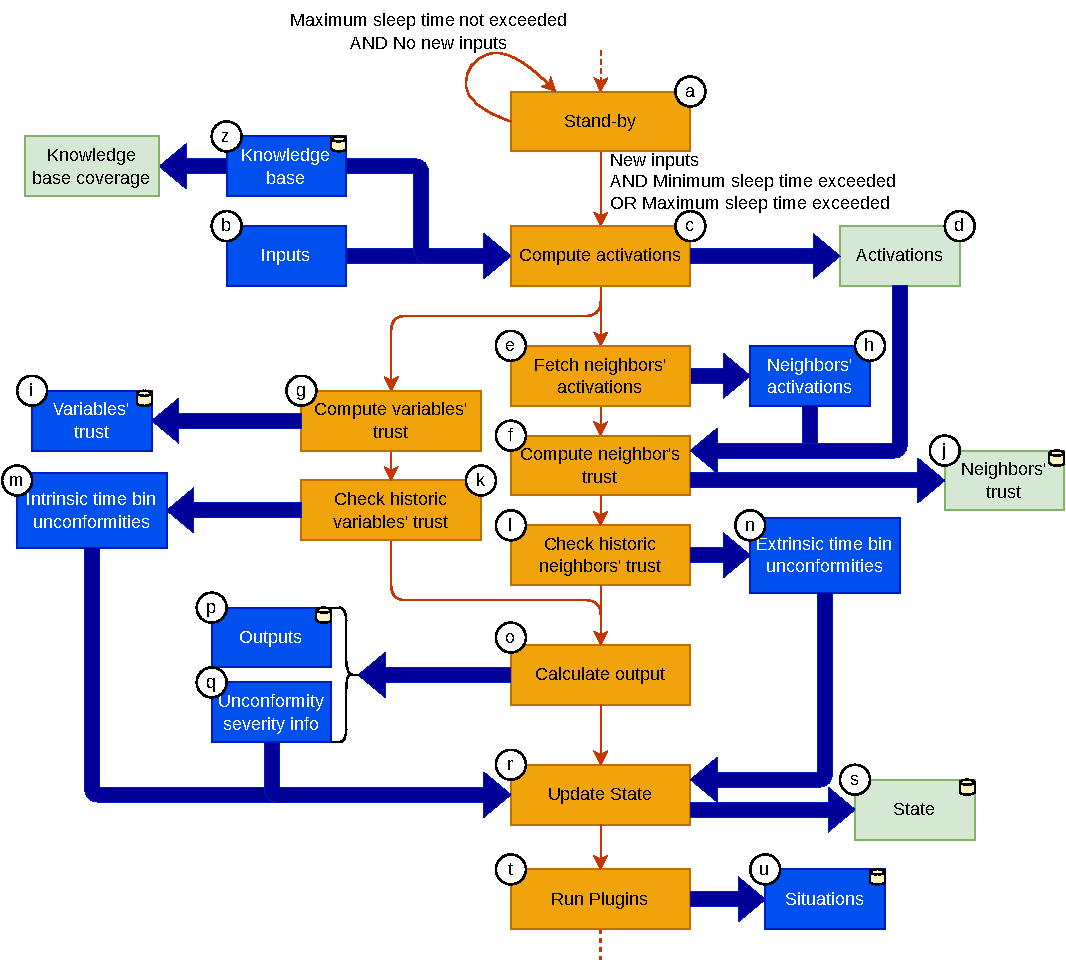
\includegraphics[width=12cm]{figures/chapter4/cell/processes.pdf}
    \caption{The cell's core sequence of processes (colored orange) and flow of data (colored blue).}
    \label{fig:cellprocesses}
\end{figure}

Figure \ref{fig:cellprocesses} showcases the cell's core procedures. It starts in a standby mode, which is only left when new information arrives or a predetermined amount of time has passed. This mode ensures no unnecessary computational burden of repeating all other computations: they provide the most valuable results when new data is available. Nonetheless, defining a maximum sleep time ensures the cell's activations are periodically updated to reflect the neighbors' state and intrinsic uncertainty.

The process of computing activations relates to the temporal similarity extraction showcased in section \ref{subsec:tempsim}. It occurs twice because inputs only contain intrinsic information, while outputs aggregate intrinsic and extrinsic data (information from neighbors), and the latter is more worthy to the network. The cell makes this procedure's byproduct (Activations) publicly available, pictured in figure \ref{fig:celldata}.

Fetching neighbor's activations 

\begin{figure}[h!]
    \centering
    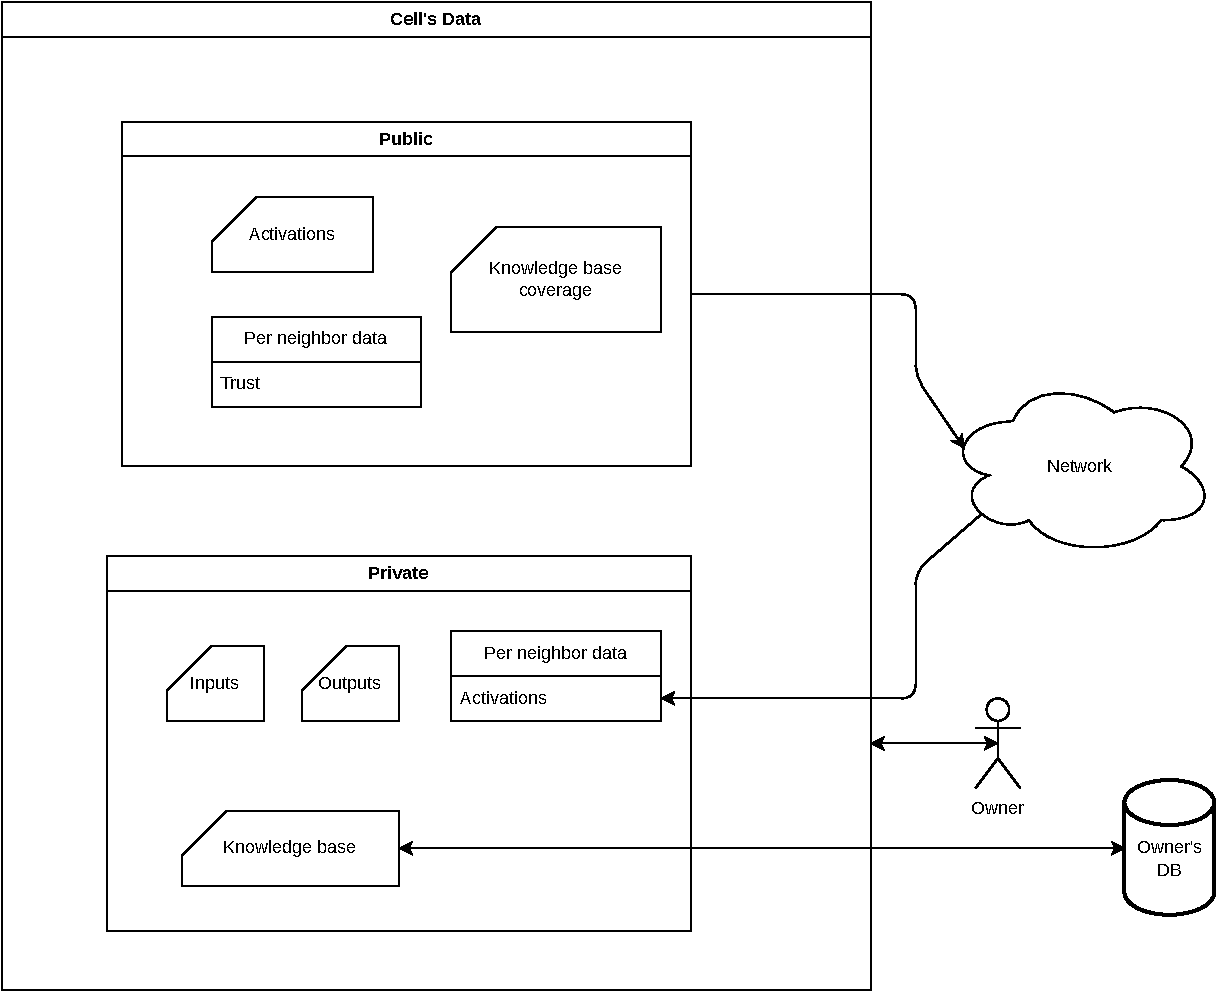
\includegraphics[width=\linewidth]{figures/chapter4/cell/data.pdf}
    \caption{The cell's public and private data attributes.}
    \label{fig:celldata}
\end{figure}

Figure \ref{fig:celldata} showcases the cell's public and private data attributes. The network may have access to its activations, knowledge base coverage, and neighbors' trust. Conversely, the cell extracts neighbors' activations from the network and gives its owner exclusive access to inputs, outputs, and knowledge base. The cell's knowledge base might only represent an interface with a private database (thus a bidirectional connection), not the data itself, since the owner might prefer a centralized storage server. The relationship between the owner and private cell data is bidirectional because it is his responsibility to update the inputs.


% TODO explicar processos da célula por alto

\subsection{Inputs and Outputs}

The cell has inputs and outputs. Both are a view of the values that define its variables at a given timestamp, which is continuously rolling. While inputs are directly associated with raw sampled data from the system (injected by the owner), outputs are a byproduct of internal processes. The latter should present more accurate information since it is based on internal and external data (ideally) and may be helpful for the cell's owner to assess its state.

Representing the cell's variables in a fuzzy (or probabilistic) manner can better capture the inherent uncertainty in time series data. For the cell's inner workings, we chose that inputs and outputs are not represented by crisp values but rather by classical sets. However, they are not limited to this representation, with fuzzy numbers or probability distributions as alternatives. Besides, they can be subject to a process called \textbf{time decay}, which ensures that the passage of time negatively affects uncertainty (more on section \ref{subsec:timedecay}). This mechanism increases the robustness of the cell by acknowledging the value of time in assessing its current state.

Summing up, the following may characterize inputs and outputs:

\begin{itemize}
    \item Classical set: simple uncertainty band (e.g., uncertainty up, down, relative, etc);
    \item Fuzzy number: generalized fuzzy number representation \cite{Zhang2019} (e.g., triangular fuzzy number (a,b,d;h));
    \item Probability distribution: the distribution's characteristics (e.g., mean ($\mu$) and standard deviation ($\delta$) for Gaussian, the mean rate of occurrence ($\lambda$) for Poisson, etc.);
\end{itemize}

\begin{figure}[h!]
    \centering
    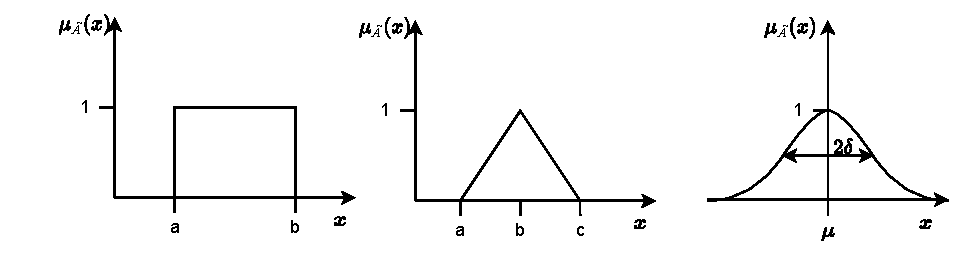
\includegraphics[width=15cm]{figures/chapter4/cell/classic_fuzzy_gaussian.pdf}
    \caption{Classical set, triangular fuzzy number, Gaussian distributions, and the associated membership function.}
    \label{fig:classicfuzzygaussian}
\end{figure}

Classical sets have pros and cons: many operations become more efficient compared to the alternatives, but we lose density information. Filtering historical data becomes trivial: a value lies within the bounds of the interval (membership value of one) or does not (membership value of zero). This more accessible representation will benefit some cell processes, primarily in temporal similarity extraction (\ref{subsec:tempsim}).

\subsection{Time decay} \label{subsec:timedecay}

In real-world dynamic systems that involve data acquisition, the certainty of the data collected tends to fade over time due to its dynamic nature. Typically, the most recent data is the most accurate representation of the system's current state, and as time elapses, the accuracy of previous data points decreases. As a result, it is crucial to consider the time dimension when analyzing dynamic systems and to develop methods that can account for the decay in data certainty over time.

As stated before, and towards considering the time dimension for the current state of a cell, we formulate a \textbf{time decay} method to ensure a more truthful and reliable assessment of the cell's current state. During the standby stage, this process ensures that the inputs and outputs suffer an increase in uncertainty.

Consider the following example of converting a crisp value (5) and uncertainty ($\pm$1) to a classical set:

$$x = 5 \pm 1 \rightarrow [5-1, 5+1] = [4, 6]$$

To simulate the increase in uncertainty over time, we suggest the following equations (\ref{eq:uncertain_down} and \ref{eq:uncertain_up}), applied to each bound:

\begin{equation} \label{eq:uncertain_down}
lower = lower - (lower - minimum) \times \frac{age}{decay}
\end{equation}

\begin{equation} \label{eq:uncertain_up}
upper = upper + (maximum - upper) \times \frac{age}{decay}
\end{equation}

The $age$ variable refers to the time difference between the present time and the instant of data acquisition. For implementation, the time unit considered is the 'second'. The $decay$ is a parametrized constant (same unit as $age$) that defines the time it takes for the set to expand into its limits when starting from the median. It is chosen based on the characteristics of the variable, i.e., knowledge of its uncertainty over time. However, a good starting point is defining close to the data acquisition period so that the set expands entirely until a new value is acquired.

\begin{figure}[h!]
    \centering
    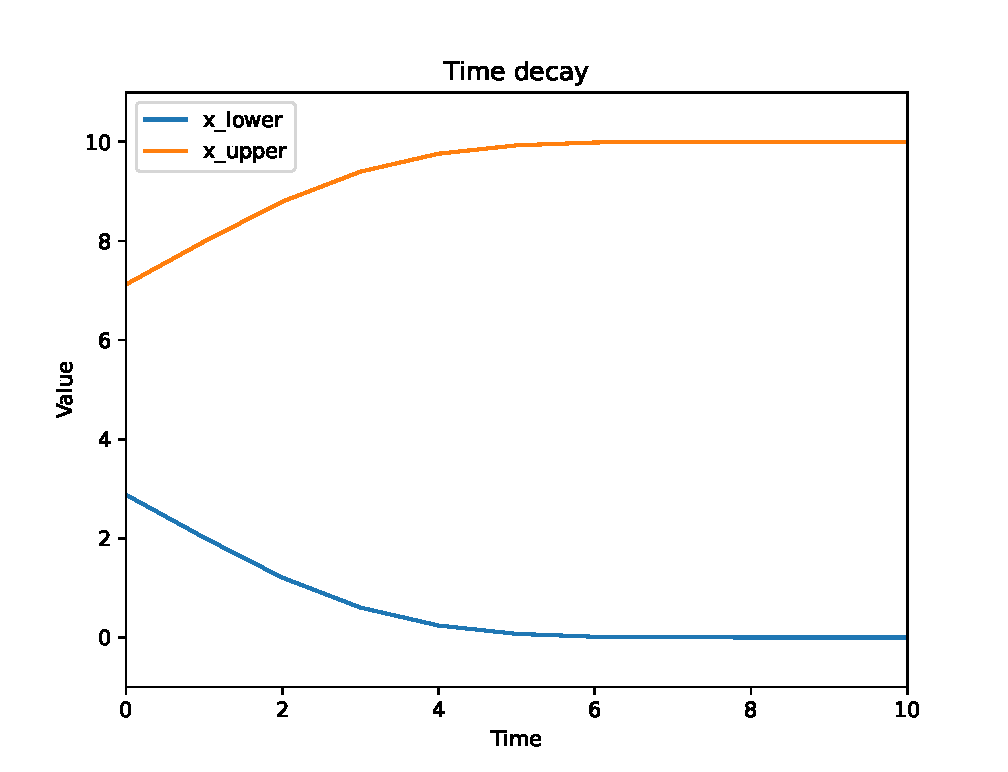
\includegraphics[width=10cm]{figures/chapter4/cell/time_decay.pdf}
    \caption{Visualization of the effect of time decay on $x_{lower}$ and $x_{upper}$.}
    \label{fig:timedecay}
\end{figure}

Figure \ref{fig:timedecay} represents the expansion of the set throughout a period equal to the decay parameter (ten seconds). When $x$ reaches the age of ten seconds, its set represents complete uncertainty since its bounds become similar to the variable limits ($x_{min}$ and $x_{max}$). We can see that the decreasing difference between the bounds and maximum/minimum values causes attenuation in the decay curve, as it displays a non-linear behavior. This behavior seems appropriate according to the reality of systems: as a variable becomes more uncertain with time, there is less potential for its uncertainty to increase.


\subsection{Temporal similarity extraction} \label{subsec:tempsim}

Temporal similarity extraction is the process of identifying recurring patterns in time series data. It involves the identification of past instances where the current state is observed to extract useful information about the system's behavior over time. By identifying historical periods with similar conditions, temporal similarity extraction can help assess the current state or predict future trends. This technique is common in statistics for purposes such as estimation and forecasting.

Using sets or probability distributions to filter historical data is one approach to simplify the process of temporal similarity extraction in multivariate time series data while also making it more robust against noisy or incomplete data. This approach assigns membership values to each data point in the time series based on the corresponding set (or distribution) generated from the current cell inputs. By eliminating samples past a certain threshold, we can form the outputs. The possibility of this process is one of the reasons for deciding to represent the inputs and outputs of the cell in a fuzzy manner. 

The proposal for similarity extraction in the cell consists of receiving new values (inputs) for the cell's variables from a data source (sensors or other data acquisition equipment, calculations, forecasting, etc.), generating a classical set, fuzzy number, or probability distribution from them, and then applying the bounds/membership function or probability density function to the knowledge base (see figure \ref{fig:solo_state_estimation}). When historical samples are associated with membership values, there may be a process for determining outputs by combining data and membership values.

The initial choice is to use classical sets since filtering history becomes trivial and efficient: restrict the knowledge base to samples where all variables belong to the corresponding interval. Generating outputs with these can be as simple as constructing new sets based on the bounds of filtered knowledge (samples with membership equal to one). When filtering historical data with two or more variables, there is a trend of narrowing down the resulting data's space due to the intersection of constraints. Therefore, this process should result in sets that are an equal or better assessment of the present state (than the sets generated by inputs). However, filtering might also result in zero samples (membership value of zero on all knowledge base's rows), which indicates not having "memory" of any similar occurrence. This zero-sample filter is an excellent indicator for potentially anomalous scenarios, primarily if we know that the knowledge base is statistically representative of the variables in the cell.

This process also makes possible for simple forecasting. Considering an offset (arbitrary number of rows forward) in the activations, the temporal similarity extraction and computation of outputs results in future values. So, cells may either compute outputs related to the present or future. Nonetheless, this temporal shift might be difficult to achieve if data samples arrive at randomly spaced intervals of time, thus would only be straightforward for systems with time-consistent data acquisition.

The following examples consider that $t=0$ is associated with the present, and $\mu$ represents membership functions.

\paragraph{Self-similarity}

With a knowledge base and input variables, the cell can perform intrinsic temporal similarity extraction.
Consider a cell characterized by two variables that are a function of time: $x(t)$ and $y(t)$,
let us assume that, at a given instant, these are the new inputs:

\begin{equation}
    x(0) = 1.0 \rightarrow \mu_{x(0)}(x) =
    \begin{cases}
        1, & x \in [0.9, 1.1]    \\
        0, & x \notin [0.9, 1.1] \\
    \end{cases}
\end{equation}

\begin{equation}
    y(0) = 2.0 \rightarrow \mu_{y(0)}(y) =
    \begin{cases}
        1, & y \in [1.8, 2.2]    \\
        0, & y \notin [1.8, 2.2] \\
    \end{cases}
\end{equation}

The membership functions $\mu$ are generated considering that $x$ and $y$ are characterized by uniform and symmetrical uncertainty and that the received samples of $x(0)$ and $y(0)$ represent their median.

\begin{figure}[h!]
    \centering
    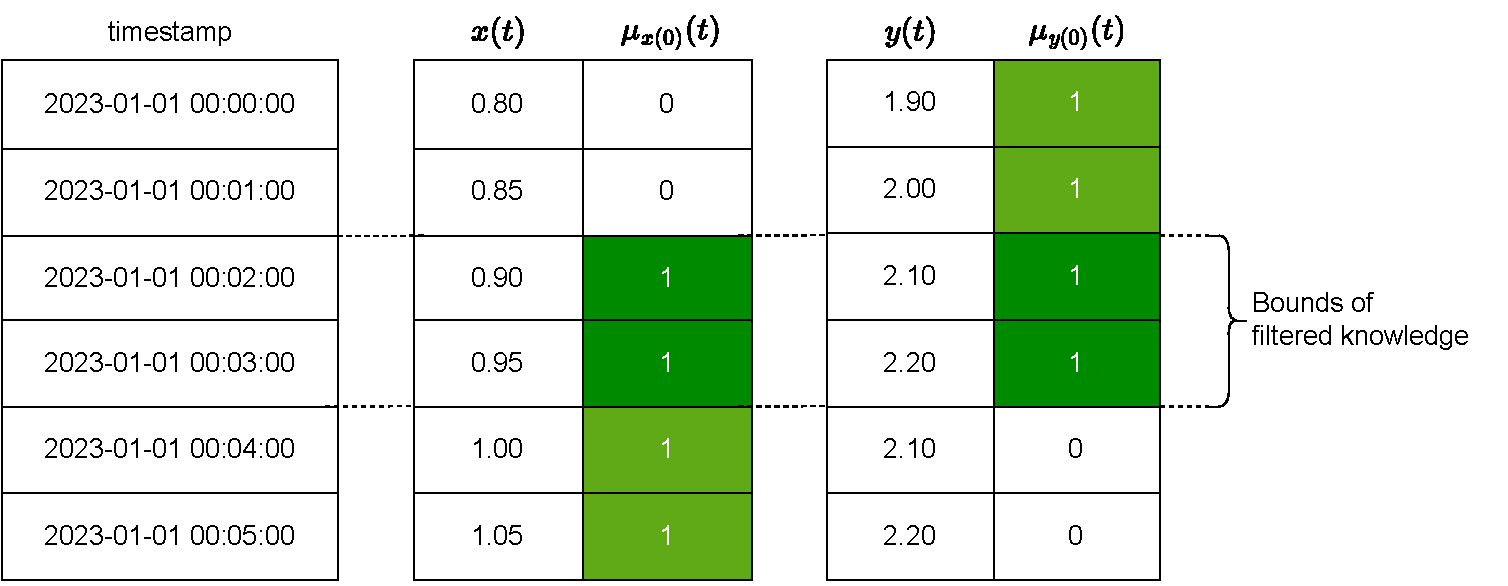
\includegraphics[width=\linewidth]{figures/chapter4/cell/solo_state_estimation.pdf}
    \caption{Visualization of a self-similarity extraction example.}
    \label{fig:solo_state_estimation}
\end{figure}


With the knowledge base represented in figure \ref{fig:solo_state_estimation}, the resulting activations will be 2023-01-01 00:02:00 and 2023-01-01 00:03:00. These are the timestamps of past instances where the cell's variables have values belonging to the set generated from new inputs. Now we can also infer that the actual values of $x$ and $y$ should reside in a set constrained by the filtered historical data ($x(t)$ and $y(t)$). Therefore, the outputs based on self-similarity extraction are:

\begin{equation}
    x'(0) \in [0.90, 0.95]
\end{equation}

\begin{equation}
    y'(0) \in [1.80, 2.20]
\end{equation}

These results confirm that we achieve outputs with less uncertainty only depending on intrinsic processes and private data.

\paragraph{Mutual Similarity}

Extending similarity extraction to multiple cells is a relatively trivial process. Suppose a cell has access to another's activations at the same rolling timestamp and for a historical window that intersects its knowledge base. In that case, it can use that information to refine the intrinsic temporal similarity extraction result. Using sets, this can occur by joining intrinsic and extrinsic membership values by aggregation (e.g., sum, multiplication, average, etc).
Although simple, this process has some tricky requirements, such as not allowing a time difference between the computation of membership values of different cells to avoid joining incoherent information, and 
% Capacidade de estimação de estado intrínsica + extrínsica


\subsection{Trust between Cells}  \label{subsec:trust}


After recognizing the potential for time similarity extraction, we discovered an additional possibility with activations. Since these represent past cell instances that exhibit similar behavior to the current inputs, we can compare them between cells. This unique characteristic of the CellTAN enables its usage without data privacy issues and not requiring data normalization. However, the knowledge base must intersect for a time-based comparison to make sense, and it yields the best results if outliers are absent.

Time possesses inherent normalization properties, as all components equally experience its passage. This characteristic enables the network to compare systems without concerns about the specific variables involved. Consequently, the proposed tool can be effectively applied beyond PV applications, showcasing its ability to be generalized across various domains.

A 2x2 contingency table represents the intersection of activations of two cells. In this table, the rows define the activation status of one cell (labeled as "Activated" and "Not Activated"), and the columns represent the activation status of the other cell (same labels).

\begin{table}[h!]
    \centering
    \caption{Contigency table representing the activation intersection of two cells.}
    \label{tab:cellactivationsintersection}
    \resizebox{8cm}{!}{%
    \begin{tabular}{ll|cc|}
    \cline{3-4}
    \multicolumn{2}{l|}{\multirow{2}{*}{}} & \multicolumn{2}{c|}{Cell 2} \\ \cline{3-4} 
    \multicolumn{2}{l|}{}                                     & \multicolumn{1}{l|}{Activated} & \multicolumn{1}{l|}{Not Activated} \\ \hline
    \multicolumn{1}{|c|}{\multirow{2}{*}{Cell 1}} & Activated & \multicolumn{1}{c|}{a}         & b                                  \\ \cline{2-4} 
    \multicolumn{1}{|c|}{} & Not Activated & \multicolumn{1}{c|}{c}  & d \\ \hline
    \end{tabular}%
    }
\end{table}

Each element of the matrix represented in Table \ref{tab:cellactivationsintersection} ($a$,$b$,$c$, and $d$) corresponds to a specific combination of activations, such as "Activated-Activated," "Activated-Not Activated," "Not Activated-Activated," and "Not Activated-Not Activated". They represent the frequency or count of observations falling into that specific combination. The main diagonal relates to the cells' agreeableness, while the secondary diagonal is the opposite: disagreeableness. For the application at hand, the 'second' is utilized, meaning that, for example, $a$ is the total amount of seconds both cells are active.

\subsubsection{Statistical tests for measuring association}

In statistics, numerous tests are available to measure the association between variables in contingency tables. One of the most known tests is Pearson's chi-square test (\ref{ap1:pearsonschi}), which assesses whether there is a significant association between the two variables. It compares the observed frequencies in the contingency table with the expected frequencies under an assumption of independence. If this test yields a statistically significant result, it suggests a non-random association between the activations of the two cells.

Another widely employed test is Fisher's exact test (\ref{ap1:fischer}), as an alternative to the chi-squared, which is particularly useful for small sample sizes. It calculates the probability of obtaining the observed distribution of activations in the contingency table, also assuming independence between the variables. If this probability is sufficiently low, it implies that the association between the activations is unlikely to occur by chance. The odds ratio and relative risk can also quantify the strength and direction of the association between two variables. The odds ratio would compare the odds of activation in one cell close to the other, while the relative risk compares the risk of activation in one cell to the risk in the other.

Considering that the desired outcome of activation comparison between cells is a normalized index that translates into how much they conform to each other (hence the term "trust"), there is a preference for inherently normalized tests, such as the $\phi$ coefficient (\ref{ap1:phi}), contingency coefficient (\ref{ap1:contingencyc}), and Theil's U (\ref{ap1:theilsu}). The goal is that this index represents how much the historical incidence of two cells' states match.

The $\phi$ coefficient, also known as Matthews correlation coefficient, is a measure of association designed explicitly for 2x2 contingency tables, quite popular in machine learning for measuring the quality of binary classification. It ranges from -1 to 1, where 0 indicates no association, -1 represents a perfect negative association, and 1 represents a perfect positive association. The contingency coefficient extends this coefficient's usability, allowing its application in larger contingency tables, and ranges from 0 to 0.707 (no association to strong association).
Finally, another relevant test is Theil's U . It accounts for the variables' mutual information and entropy based on information theory principles, providing a measure for the proportion of total entropy in one variable that the other can explain. It also ranges from 0 to 1.

\subsubsection{Proposed trust measurement method}

All the mentioned tests may offer different perspectives on the association between the activations of two cells. However, none are considered adequate for our application, so we propose a new method, defined by \ref{eq:cdmchi}.

\begin{equation} \label{eq:cdmchi}
    \chi_a^{2'} = \frac{(p_a - E(p_a))^2}{E(p_a)}
\end{equation}

Where:

\[
    p_a = \frac{a}{a+b+c+d}
\]

\[
    E(p_a) = \frac{(a + c) \times (a + b)}{(a+b+c+d)^2}
\]

\begin{align*}
    p_a &: \text{Probability of both cells being active} \\
    E(p_a) &: \text{Expected value for the probability of both cells being active}
\end{align*}

Based on Pearson's chi-squared test, this new approach focuses on the "a" component: the pure agreeableness between two cells. Its value ranges from 0 to 1 (no "trust" to complete "trust"). Some of the most relevant tests previously presented, namely the $\phi$ coefficient, contingency coefficient, and Theil's U, are compared to this new method for comparison and validation in the following experiments.

\subsubsection{Experiments}

\paragraph{Experiment nº1}

The first trial simulates the variation of the $d$ component and its effect on some association coefficients. It's expected that, as not activated time increases, the chance of the two cells intersecting activations lowers, and so their trust should increase. The starting point and used spaces of $d$ are:

$$
\begin{bmatrix}
    30 & 10 \\ 10 & d
\end{bmatrix}
$$
$$
d \in [0, 100], d \in [0, 3000]
$$

\begin{figure}[h!]
\centering
    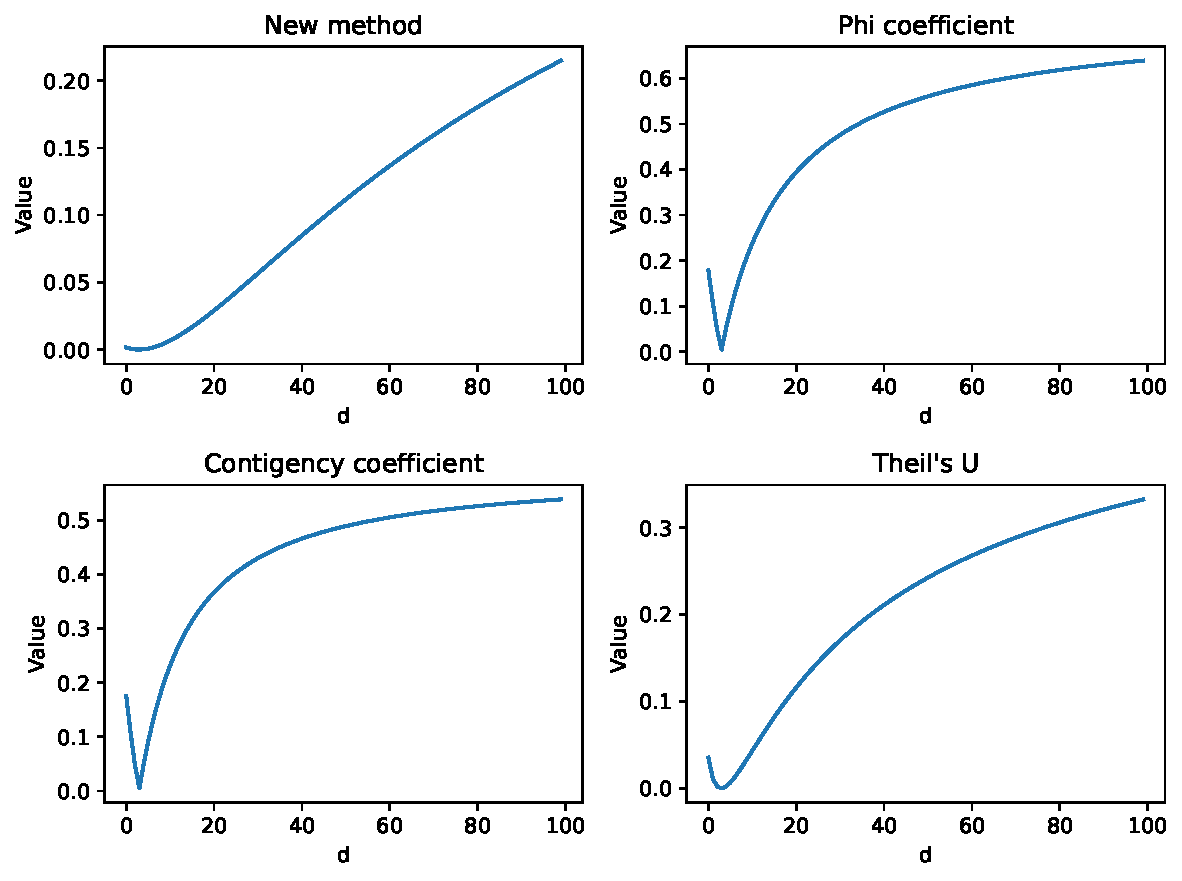
\includegraphics[width=0.8\textwidth]{figures/chapter4/cell/trust_tests/1_a.pdf}
    \caption{Trust measurement evolution for different methods with $a=30, b=10, c=10, d \in [0, 100]$.}
    \label{fig:trust_test_1_a}
\end{figure}
\FloatBarrier


In figure \ref{fig:trust_test_1_a}, we can observe that all measurements increase with $d$, with a slight reduction at the start, although attenuated on the new method. Theil's U's minimum is 0.5, while the expectation for having a lower $d$ (few deactivated intersecting periods) is a value closer to zero (as the other methods demonstrate). This scenario means either both cells have no history similar to current inputs or their inputs' values have significant uncertainty (remember the time extraction process from \ref{subsec:tempsim}). Therefore, their "trust" should be minimal.
Not having a reduction in the first values of $d$, showcased by the new method, is the intended behavior. Having equal activated and deactivated intersections ($a$ and $d$) should not be significantly penalized versus having $a>>d$, justified by the above reasoning.

\begin{figure}[h!]
\centering
    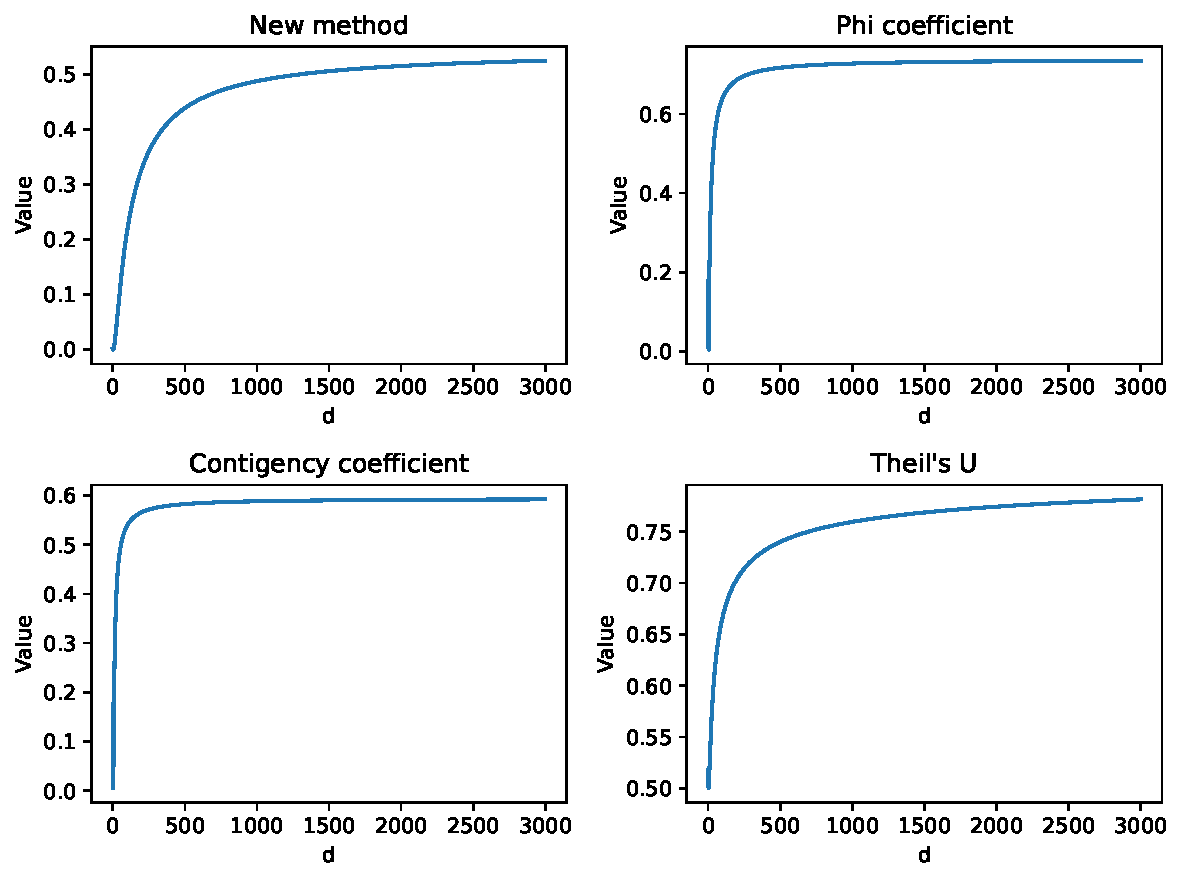
\includegraphics[width=0.8\textwidth]{figures/chapter4/cell/trust_tests/1_b.pdf}
    \caption{test 1 b}
    \label{fig:trust_test_1_b}
\end{figure}
\FloatBarrier

Figure \ref{fig:trust_test_1_b} extends the previous analysis, showcasing that all methods have asymptotical behavior, settling in a value greater than the start. All except Theil's U have asymptotes deemed acceptable for this test: since disagreement terms $b$ and $c$ are non-null and relatively close to $a$, we expect that the trust index does not reach a value near the max, remaining closer to a measure of "half trust".

\paragraph{Experiment nº2} Now, we observe the impact of the disagreeing terms $b$ and $c$ in the same coefficients by varying one while maintaining all others fixed. The expectation is that an increase in disagreement should lead to zero trust.

$$
\begin{bmatrix}
    30 & b \\ 10 & 10
\end{bmatrix}
$$
$$
b \in [0, 1000]
$$
\begin{figure}[h!]
\centering
    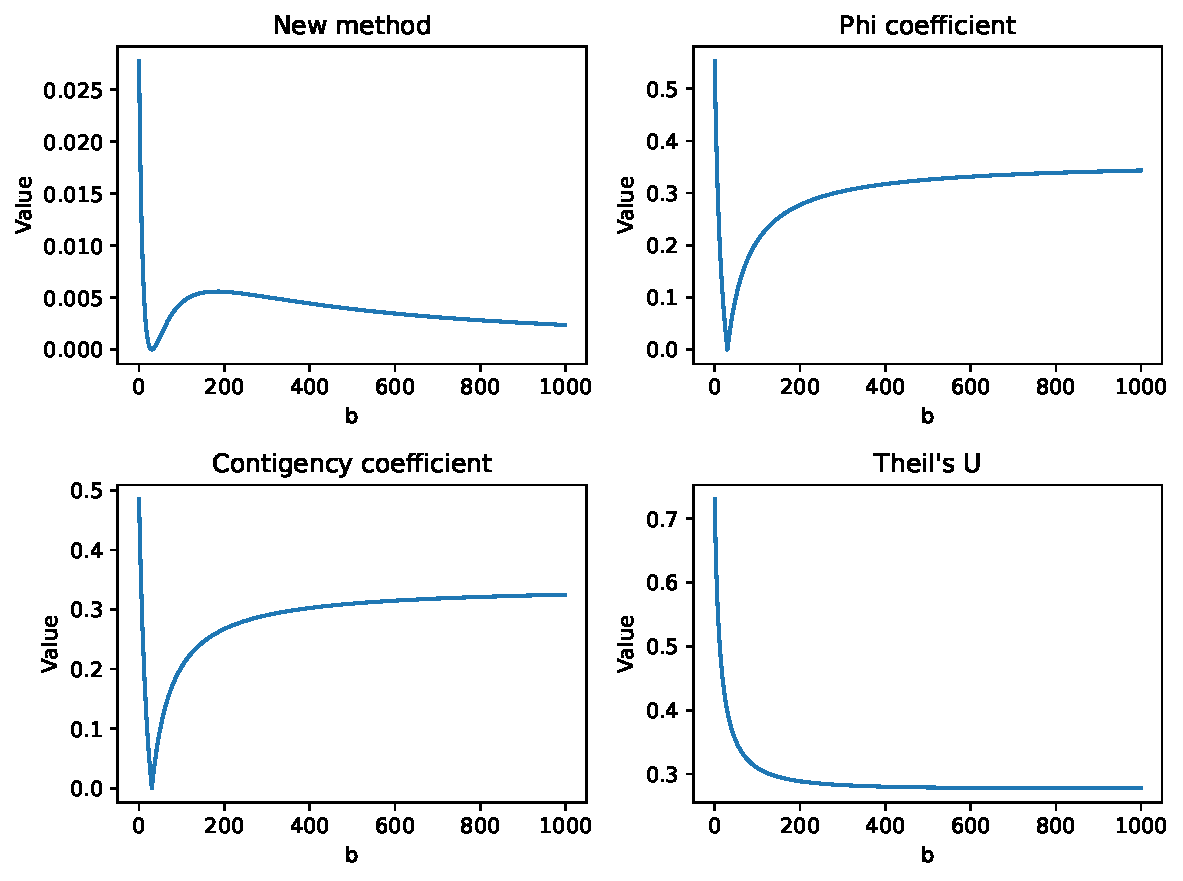
\includegraphics[width=0.8\textwidth]{figures/chapter4/cell/trust_tests/2_a.pdf}
    \caption{test 2 a}
    \label{fig:trust_test_2_a}
\end{figure}
\FloatBarrier

In figure \ref{fig:trust_test_2_a}, it is clear that, for all methods, an increase in $b$ leads to lower coefficients. All except the new algorithm tend towards similar asymptotes, near a value of 0.3. The expected behavior is precisely met by the new method.

$$
\begin{bmatrix}
    30 & 10 \\ c & 10
\end{bmatrix}
$$
$$
c \in [0, 1000]
$$
\begin{figure}[h!]
\centering
    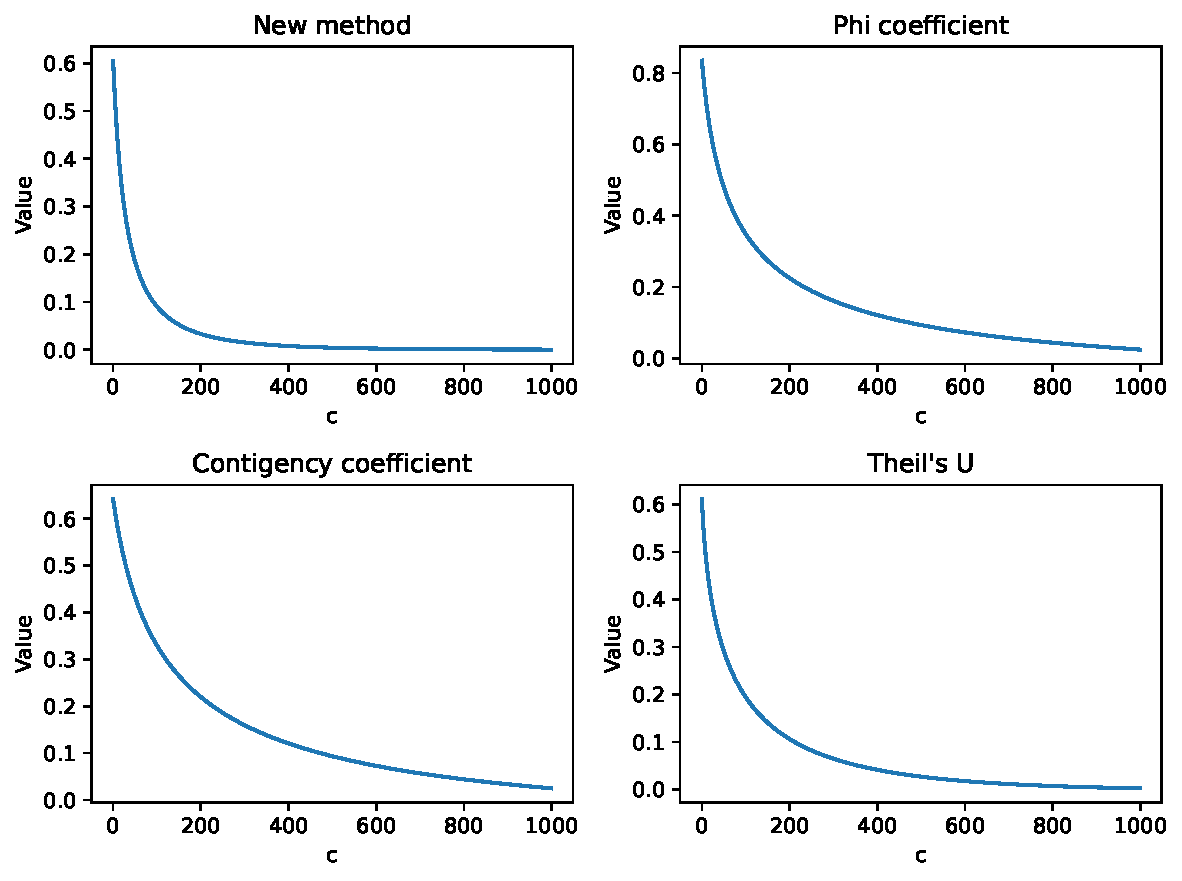
\includegraphics[width=0.8\textwidth]{figures/chapter4/cell/trust_tests/2_b.pdf}
    \caption{test 2 b}
    \label{fig:trust_test_2_b}
\end{figure}
\FloatBarrier

With figure \ref{fig:trust_test_2_b}, we can observe the asymmetry of Theil's U coefficient, opposing to what figure \ref{fig:trust_test_2_a} showed. It does not represent the trust between cell nº1 and cell nº2, but the trust of cell nº1 \textbf{in} cell nº2. The rest of the methods have symmetrical coefficients, thus presenting the same results.

\paragraph{Experiment nº3} This last experiment showcases the effect of changing term $a$. When the cells share an increasing amount of activated time, assuming their trust should increase is trivial. However, reasoning that having a disproportionally ample activated time means there is more uncertainty on their current state, then trust should lower. The expectation is that, as $a$ increases, there is also an increase in trust until a specific peak. It should decrease after reaching a global maximum and have an asymptote at zero.

\begin{figure}[h!]
\centering
    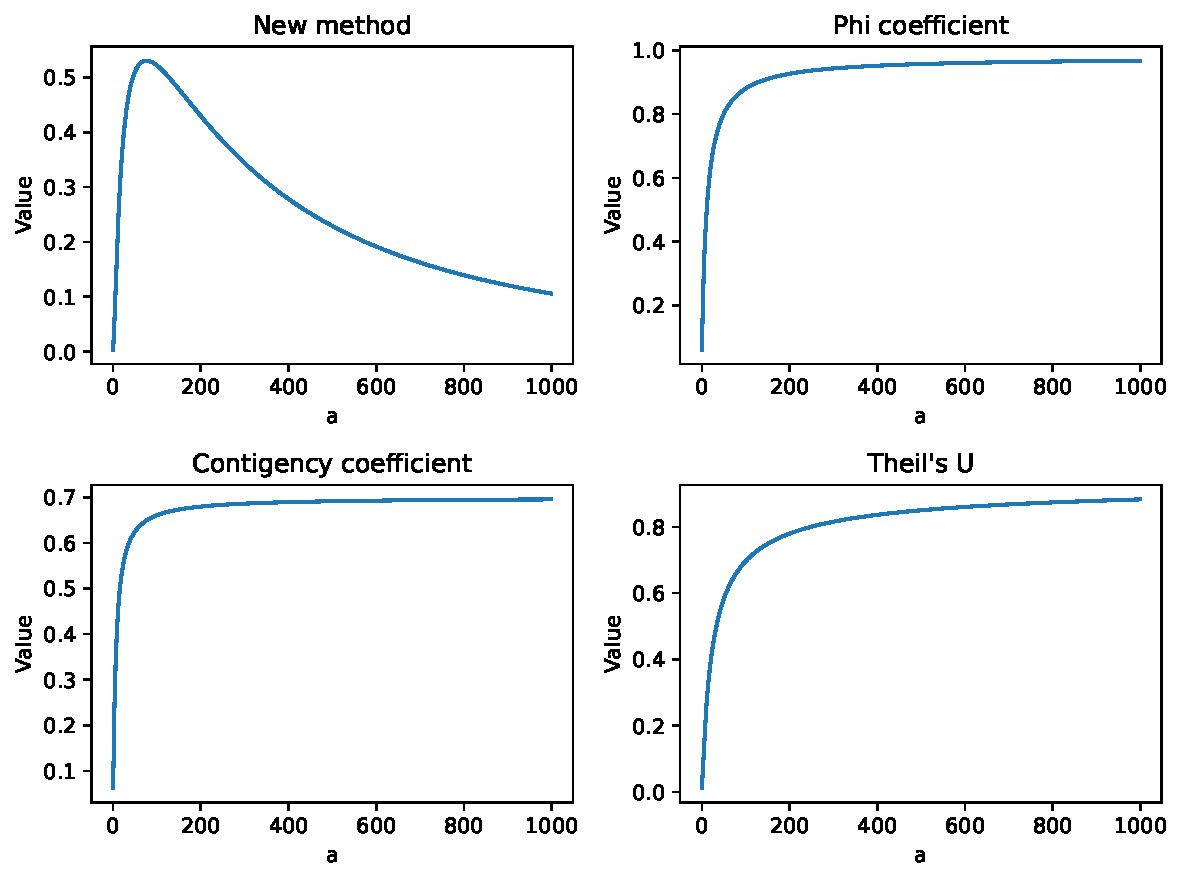
\includegraphics[width=0.8\textwidth]{figures/chapter4/cell/trust_tests/3.pdf}
    \caption{test 3}
    \label{fig:trust_test_3}
\end{figure}
\FloatBarrier

Figure \ref{fig:trust_test_3} shows that only the new method presents the previously described "goal" behavior. Otherwise, all other coefficients approach their max when $a$ tends towards infinity.

With the three experiments presented, we confirm that the proposed approach for computing the trust index between cells is better suited, considering the requirements and assumptions.

\subsection{Connections}

Mutual similarity extraction and trust calculation cannot occur in isolation. Therefore, connections are the essence of forming the CellTAN. These links can also have indicators for describing the cells' relationships, like the trust index, which is crucial for anomaly detection.

Each cell has a unique identifier, generated upon creation and independent of the name attributed by the owner. This ID serves to register cells and better manage the network. Since interconnections require an agent to keep track of these IDs and correctly redirect traffic, we introduce the \textbf{Hub} component. This central element provides global network visibility and makes connections easier to form and maintain. For a cell, a connection is no more than the identifier of the neighbor, which the hub can directly associate with a communication link.

On cell deployment, the system expects the owner and the CellTAN manager to manually link cells together by assigning each connection. However, the plan is to develop a mechanism that proposes new connections based on the neighbor's neighbors through the hub. This mechanism could function based on the strength of the relationship between cells and neighbors in common, recommending a direct link if both "trust" them similarly. As the last phrase hints, an indicator called "trust" is the criterion for evaluating these links. The following subsection defines the conception of this metric.

\subsubsection{Communication Protocol}

In the context of ensuring proper data sharing between cells, the choice of communication protocol is a crucial aspect of establishing connections. For this work, we implemented a local communication mode for cells running on the same machine or within the same process and a remote communication model intended for cells distributed across different servers. The local communication mode is straightforward, assuming direct links between cells within the program. However, multiple protocol options regarding remote communication exist, including HTTP, HTTPS, WebSocket, and MQTT (excluding protocols for wireless proximity communication, as the CellTAN system assumes cells may be in different geographical locations). Initially, we implemented HTTP/HTTPS for remote communications due to its accessibility and ease of implementation. However, given its synchronous operation (based on request and response), we soon realized there might be more appropriate and robust choices for a distributed asynchronous system. Consequently, as future work, we should refactor the remote interface to utilize MQTT.

HTTP (Hypertext Transfer Protocol) and MQTT (Message Queuing Telemetry Transport) are communication protocols in different contexts. HTTP, a request-response protocol widely used in web applications, operates over TCP and follows a client-server model. It proves suitable when clients need to retrieve or send specific data to and from a server. HTTP is simple, widely supported, and compatible with browsers and standard web technologies. However, its stateless nature and lack of optimization for real-time communication can result in high overhead caused by frequent request-response cycles.

% TODO referencias

In contrast, MQTT is a lightweight publish-subscribe messaging protocol designed for efficient communication in distributed systems, especially within the Internet of Things (IoT). MQTT utilizes a broker-based architecture, where clients publish messages to topics and subscribe to receive messages from specific topics of interest. MQTT is highly scalable, bandwidth-efficient, and supports asynchronous messaging. It minimizes network and power consumption while providing reliable message delivery. However, implementing MQTT may require additional infrastructure, such as MQTT brokers.
The publish-subscribe model of MQTT facilitates decoupled communication between system components, allowing for scalable and flexible systems. It is suitable for scenarios where devices or services exchange information in a distributed environment asynchronously. MQTT often outshines HTTP as the preferable choice for a distributed asynchronous system emphasizing real-time data exchange and efficient communication. Nevertheless, HTTP remains the more appropriate choice if the system primarily revolves around traditional web applications and request-response interactions. Ultimately, the scope of CellTAN requires the leverage of both protocols in different aspects of the tool: HTTP is more suitable for human-system interaction, and MQTT for system-system exchanges.


\subsection{States}

We introduce a state system to summarize the results of cells' processes. The state represents a short view into intrinsic and extrinsic unconformities occuring in the cell.

\subsection{Application Plugins}

% ? Isto devia criar um capítulo inteiro só por sí não?

The broad capabilities of the CellTAN make it less insightful when extracting specific information from the cells. Although its generalized design extends usability to different types of systems, it still requires additional processes to assess particular situations beyond neighborhood or internal unconformities. During the literature review process, the specificity of algorithms is noticeable, and most techniques do not attempt to diverge from the PV application when it comes to fault detection and classification. This standard approach yields excellent results and could boost CellTAN's capabilities.

To solve the presented issue and dwell on the PV application theme of this work, we introduce the concept of \textbf{plugins}. Plugins extend the cell's core functionality, introduced to leverage specific system logic to identify patterns in its variables, like classical algorithms. When binding them to a cell, they have a setup that checks if the required variables are present in its inputs. Then, after the intrinsic processes, they can run an algorithm that assesses what current situations the cell might be experiencing. This way, the CellTAN can still work with entities of different natures while these plugins work alongside them, accessing private data and reporting sensible insights to the owner. 

To illustrate this feature, let us imagine setting up a PV inverter CellTAN representative of a solar farm. Although the tool does not "know" anything about inverters nor "cares" that the cells are of this type, the agent responsible for adding them to the network certainly does. Therefore, binding a PV-specific algorithm to assess particular inverter situations, such as malfunction, over(/under) voltage(/current), and performance degradation, is wise. This additional process makes the tool warn the owner of specific inverter faults besides possible mismatches in neighboring inverters through the generalized cell procedures.

\section{The Hub}

The CellTAN tool is supposed to be easily accessible for different assets and owners in any given location. However, for privacy and security reasons, monitoring equipment and other smart devices (IoT, servers, etc.) in PV plants and the owner's database are usually protected from unwanted outside connections. Because of this, the CellTAN network owner can act as a proxy and be responsible for arranging the necessary connections between the equipment of different asset owners and the network. This way, all traffic is routed through its system, which solves the issues mentioned before but possibly introduces a bottleneck and affects availability. These downsides are inevitable for aggregating distributed systems and sharing information between otherwise reserved agents. Besides being a proxy, other responsibilities associated with the hub are:

\begin{itemize}
    \item Provide network visibility: cells and connections;
    \item Receive events from cells;
    \item Cell connection proposal.
\end{itemize}

Adding this component permits visualizing all the cells registered in the system and their public data. This 

\section{Implementation}

\subsection{Code and Infraestructure}

Materializing both the cell and the hub happened by coding Python modules. It was developed using a mix of the OOP (Object Oriented Programming) and FP (functional programming) paradigms and features a structure familiar with the descriptions in previous sections. Using Python for the implementation of the CellTAN comes with the following advantages:

\begin{itemize}
    \item Easy to read and write code, requiring less syntax for complex operations compared to low-level languages;
    \item Extensive availability of libraries and tools;
    \item Deployment ease: does not have to compile, only needing an interpreter and dependencies to run;
    \item Big community support, with many resources publicly available online (e.g., documentation, tutorials, etc.). 
\end{itemize}

% imagem com as tecnologias em anexos talvez

Docker containers \cite{docker} are the infrastructure choice for deploying these modules (Cells and Hub). They allow running software as containerized applications, with all the necessary dependencies installed in an isolated environment. It acts as a separate system built for running the application instead of relying on the host's OS (Operating System) and running bare-metal. This execution strategy adds an isolation layer between the program and the host machine, increasing safety and making the "production" environment more predictable and stable. An overview of the technology stack utilized (and proposed) for the software products created in this work is pictured in appendix \ref{ap1:techstack}.

% dockerfile em anexos?

\subsection{Cell configuration and deployment}


Configuring cells can be done through configuration files (one per cell). They should contain the cell variables' definitions, database credentials, hub credentials, and all other parameters. Because of its simplicity, we chose the YAML serialization specification \cite{yaml} to parse these configurations. A walkthrough of the cell configuration and expected file structure is present in appendix \ref{ap1:config}


% meter anexo para explicação das configs com screenshot de configuração exemplo

\chapter{CellTAN Application} \label{chap:chap5}


\section{Case Study}


The experiments validating CellTAN's behavior incorporate two neighboring grid-tied string inverters from the same PV farm with common satellite data. Their only known characteristics are:

\begin{itemize}
    \item Inverter one: 12.5kW nominal power; 14.4kW peak power; fixed tilt and azimuth; installed January 1st, 2013.
    \item Inverter two: 15kW nominal power; 15.84kW peak power; fixed tilt and azimuth; installed January 1st, 2013.
\end{itemize}

\begin{table}[h!]
\caption{Available variables from two inverters and a satellite.}
\label{tab:availablevariables}
\resizebox{\textwidth}{!}{%
\begin{tabular}{|l|l|l|l|}
\hline
\multicolumn{1}{|c|}{\textbf{Variable}} & \multicolumn{1}{c|}{\textbf{Source}} & \multicolumn{1}{c|}{\textbf{Unit}} & \multicolumn{1}{c|}{\textbf{Label}} \\ \hline
AC side power                           & Inverter (1 \& 2)                    & W                                  & ac\_power                           \\ \hline
AC side current                         & Inverter (1 \& 2)                    & A                                  & ac\_current                         \\ \hline
AC side voltage                         & Inverter (1 \& 2)                    & V                                  & ac\_voltage                         \\ \hline
DC side power                           & Inverter (1 \& 2)                    & W                                  & dc\_power                           \\ \hline
DC side current                         & Inverter (1 \& 2)                    & A                                  & dc\_current                         \\ \hline
DC side voltage                         & Inverter (1 \& 2)                    & V                                  & dc\_voltage                         \\ \hline
Global tilted irradiance                & Satellite                            & W/m\textsuperscript{2}             & global\_tilted\_irradiance          \\ \hline
Global horizontal irradiance            & Satellite                            & W/m\textsuperscript{2}             & global\_horizontal\_irradiance      \\ \hline
Cloud coverage                          & Satellite                            & \%                                 & cloud\_coverage                     \\ \hline
Air temperature                         & Satellite                            & ºC                                 & temperature                         \\ \hline
\end{tabular}%
}
\end{table}

Table \ref{tab:availablevariables} represents the available variables and corresponding labels used to identify them in the cell's inputs and graphs. These variables are sampled every 10 minutes from May 31, 2020, at 5:00 am to April 30, 2023, at 7:30 pm (with gaps). We utilized data from 2020 until the end of 2022 for the cells' knowledge base, and any information from 2023 onwards is considered new and used for testing. Since there is no production at night, the data's original database does not store values for this period. Not accounting for the night as missing samples, we have around 98\% of data availability.

Analyzing and cleaning raw inverter and satellite data is essential to take full benefit of CellTAN's capabilities. As seen in its formulation stage, having a clean knowledge base contributes to correctly identifying anomalous situations. Therefore, the following sections focus on these two steps, contributing to understanding the anomalies' domain and frequency of occurrence.

\subsection{Data Analysis}

Before data visualization, and regarding the variables in table \ref{tab:availablevariables}, we eliminate those that will not benefit the CellTAN. We determined that AC side voltage is insignificant since the grid mandates it in a grid-tied inverter. We have decided to only use the measure of power instead of using the AC side current measure since, in conjunction with voltage, it provides the same information. To simplify things further, we do not need to consider the power on the DC if considering both the DC side current and voltage measures.

We examine all variables related to satellite data to determine which ones could be useful, not making any premature assumptions.

\subsubsection{Power}


\begin{figure}[h!]
    \centering
    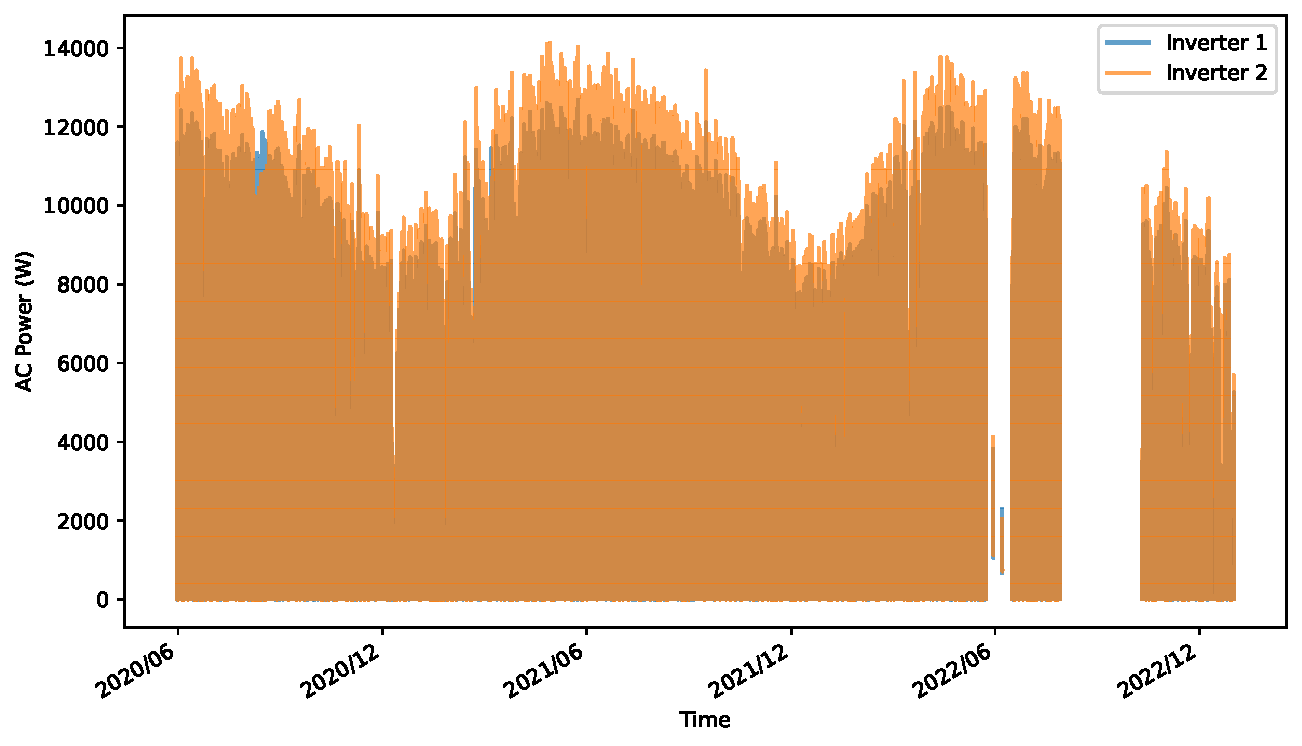
\includegraphics[width=\textwidth]{figures/chapter5/analysis/00_power_kb.pdf}
    \caption{Inverter AC side power from 2020 to 2022, used for the knowledge base.}
    \label{fig:eda_power_kb}
\end{figure}

Figure \ref{fig:eda_power_kb} shows the power profile of the two studied inverters. Right away, we notice that the power of inverter two caps at around 14kW, while inverter one usually maxes at 12kW. This information is coherent with their ratings. We can notice two relatively large chunks of missing data, with the gaps occurring in mid to late 2022.

\begin{figure}[h!]
    \centering
    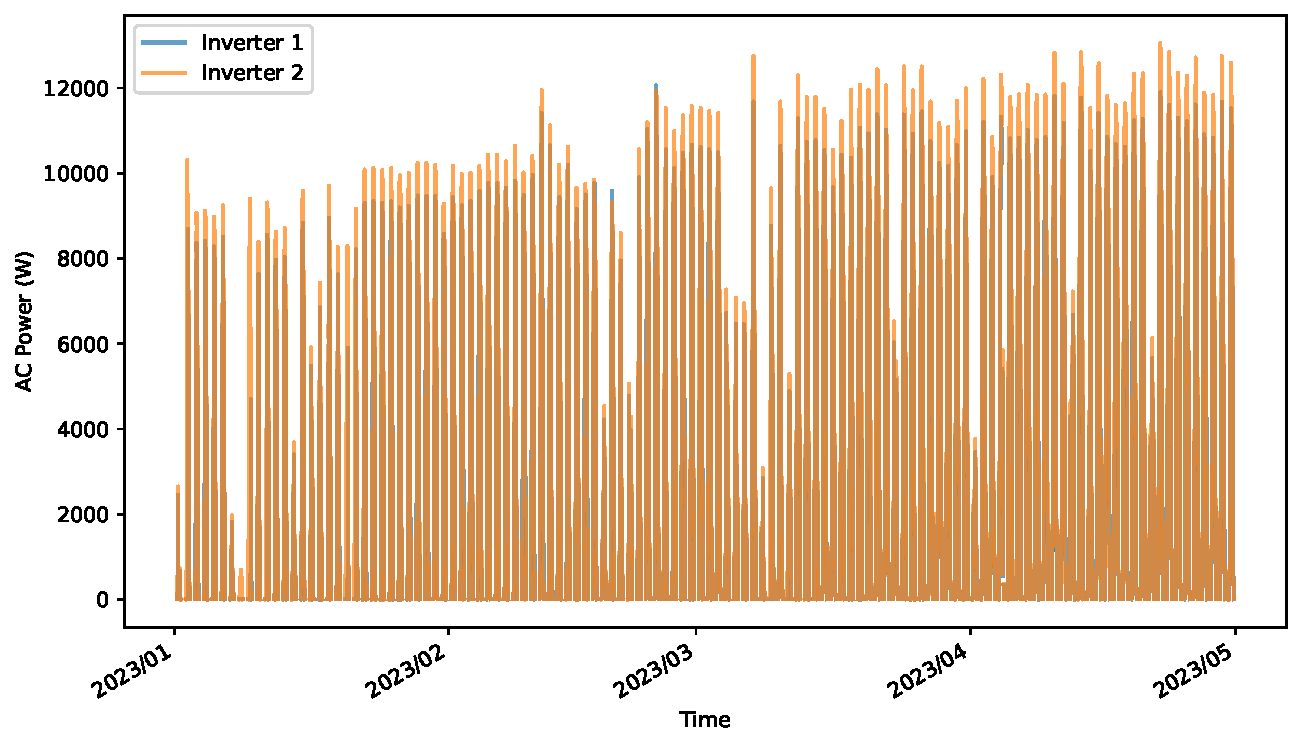
\includegraphics[width=\textwidth]{figures/chapter5/analysis/01_power_test.pdf}
    \caption{Inverter AC side power from 2023-01-01 to 2023-01-05, used for testing.}
    \label{fig:eda_power_test}
\end{figure}

Figure \ref{fig:eda_power_test} represents the power profile on the portion of data used for testing. When performing a closer inspection (with more zoom), we could hand-pick some fault occurrences in both datasets, with the majority being one inverter off while the other continues regular operation. However, these will be more noticeable during different types of data analysis, such as pair plotting. Regardless, the cases that will matter are in the test data since these scenarios will not exist in the knowledge after cleaning. In Section \ref{subsec:results}, you will find a selection of carefully chosen scenarios.

\begin{figure}[h!]
    \centering
    \includegraphics[width=\textwidth,trim={0 5.5cm 0cm 5.5cm},clip]{figures/chapter5/analysis/02_power_pairplots_kb_annotated.pdf}
    \caption{Pair plot of AC power from both inverters (2020 to 2022), using scatter (left) and KDE (Kernel Density Estimation) (right).}
    \label{fig:eda_power_kb_pair}
\end{figure}

Figure \ref{fig:eda_power_kb_pair} lets us better understand the relationship between the two inverters. As expected, since they are neighboring, this data presents a strong trend line, loading to a high Pearson coefficient: 0.97753. However, the noise from outliers is noticeable in the scatter. We define Zone A as the zone where inverter two underperforms compared to one and Zone B as the opposite. The black arrows \textcircled{\raisebox{-0.9pt}{1}} in the graph display secondary trend lines, indicating scenarios of inverter one performing consistently less than expected. Another arrow \textcircled{\raisebox{-0.9pt}{2}} also points out a cloud in Zone A (right under the trend line) of the opposite scenario. Furthermore, the red rectangles \textcircled{\raisebox{-0.9pt}{3}}\textcircled{\raisebox{-0.9pt}{4}} highlight instances where one inverter was functioning while the other was not. CellTAN must flag these situations, so we should remove them from the knowledge base. The KDE visualization confirms that most samples lie close to the primary trend.

\begin{figure}[h!]
    \centering
    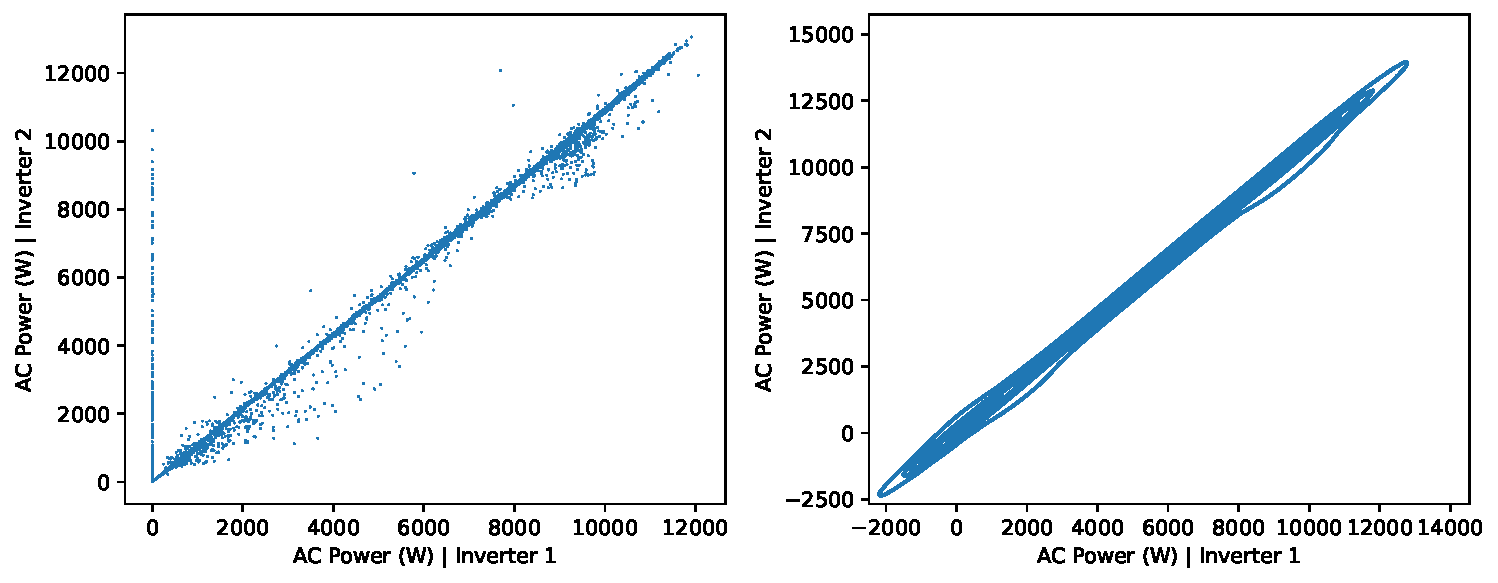
\includegraphics[width=\textwidth]{figures/chapter5/analysis/03_power_pairplots_test.pdf}
    \caption{Pair plot of AC power from both inverters (2023), using scatter (left) and KDE (Kernel Density Estimation) (right).}
    \label{fig:eda_power_test_pair}
\end{figure}

From \ref{fig:eda_power_test_pair}, it is clear that test data has fewer outliers than the previous. Nonetheless, there are many occurrences of inverter one being inoperational. Besides, there are also a considerable amount of samples below the trend line, meaning the underperformance of inverter two.

% dizer que tem menos outliers, mas várias situações com o inversor 1 inoperacional

\subsubsection{Voltage and Current} \label{subsubsec:eda_volt_curr}

Both inverters are equipped with MPPTs to maximize the power output from their strings. As a result of this power converter, the current and voltage readings should fall within the optimal range of the I-V curve.

\begin{figure}[h!]
    \centering
    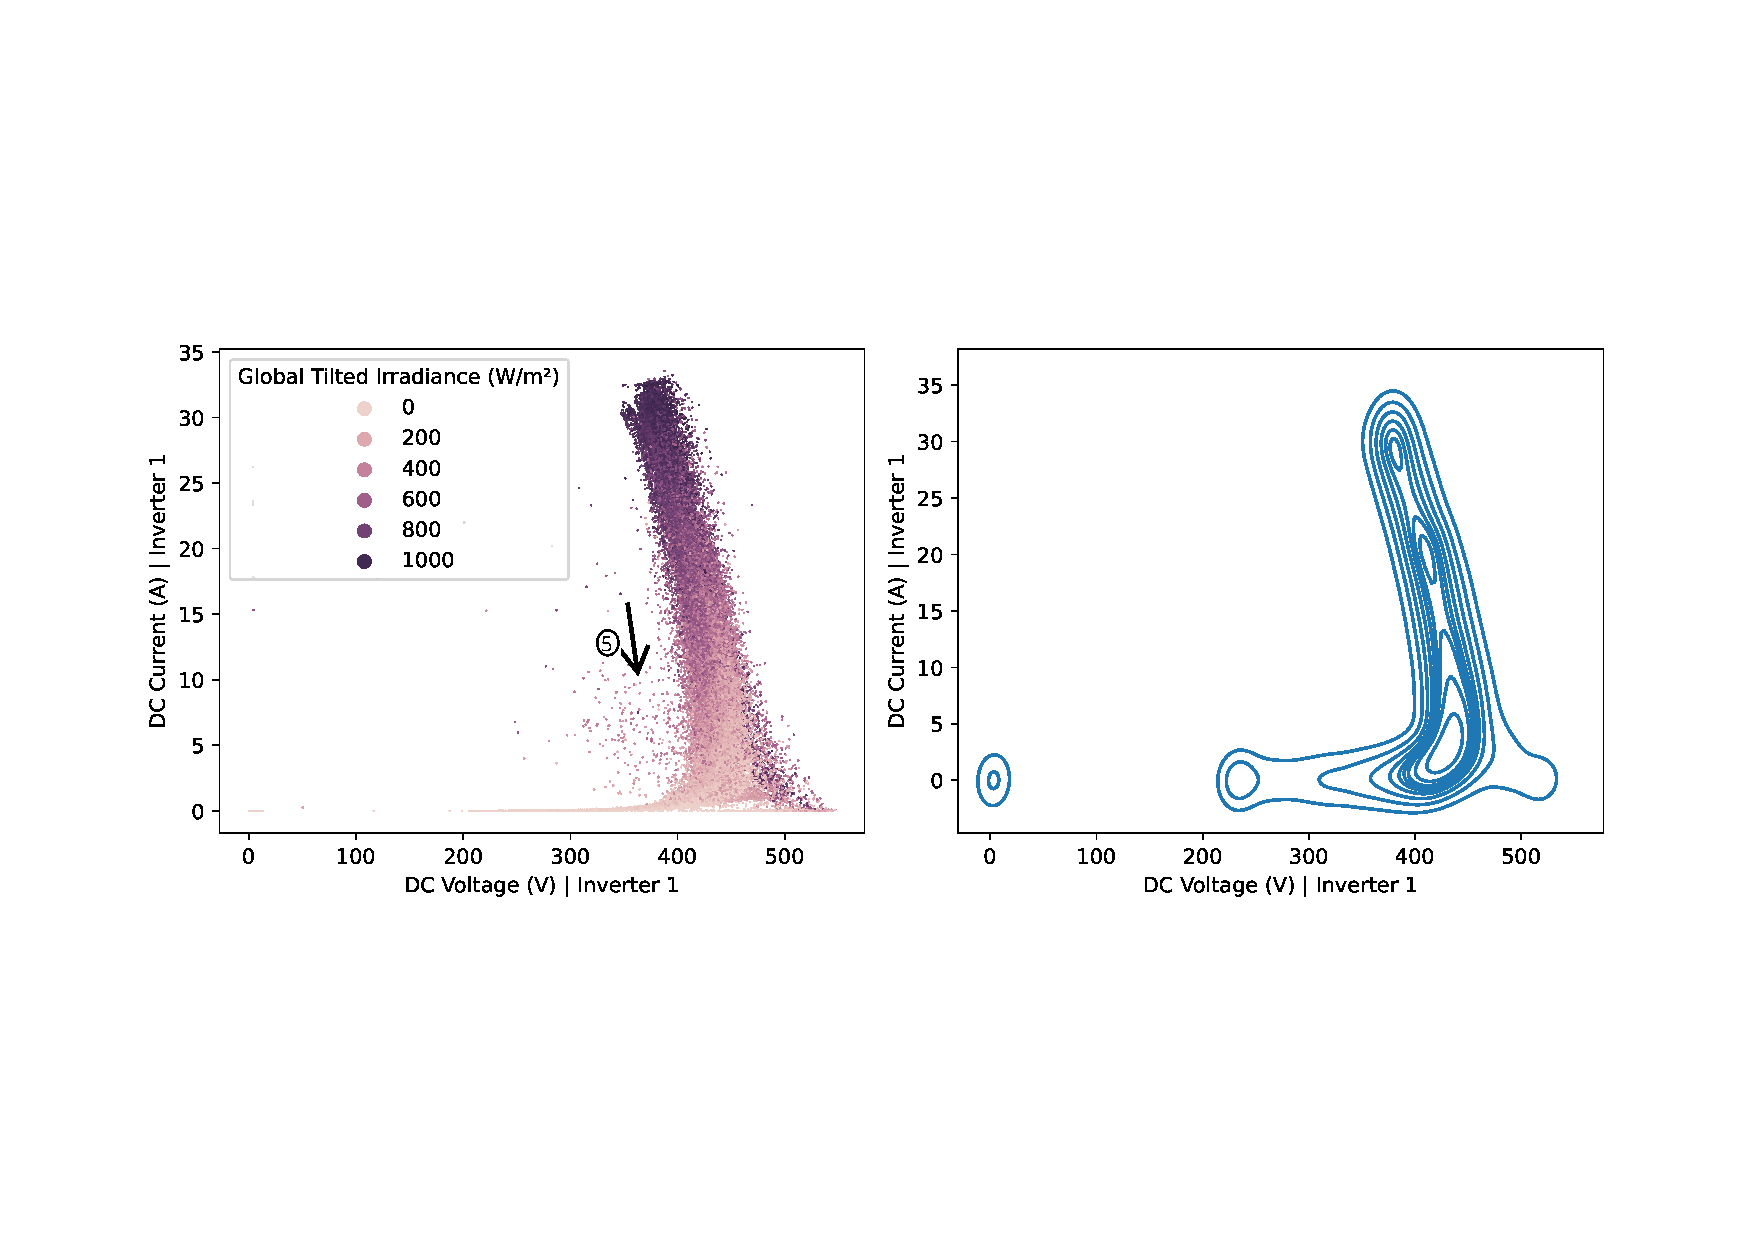
\includegraphics[width=\textwidth,trim={0 5.5cm 0cm 5.5cm},clip]{figures/chapter5/analysis/04_voltage_current_pairplot_kb_1_annotated.pdf}
    \caption{Pair plot of DC side voltage and current from inverter one (2020-2022), using scatter (left) and KDE (Kernel Density Estimation) (right).}
    \label{fig:eda_volt_curr_pair_kb_1}
\end{figure}

\begin{figure}[h!]
    \centering
    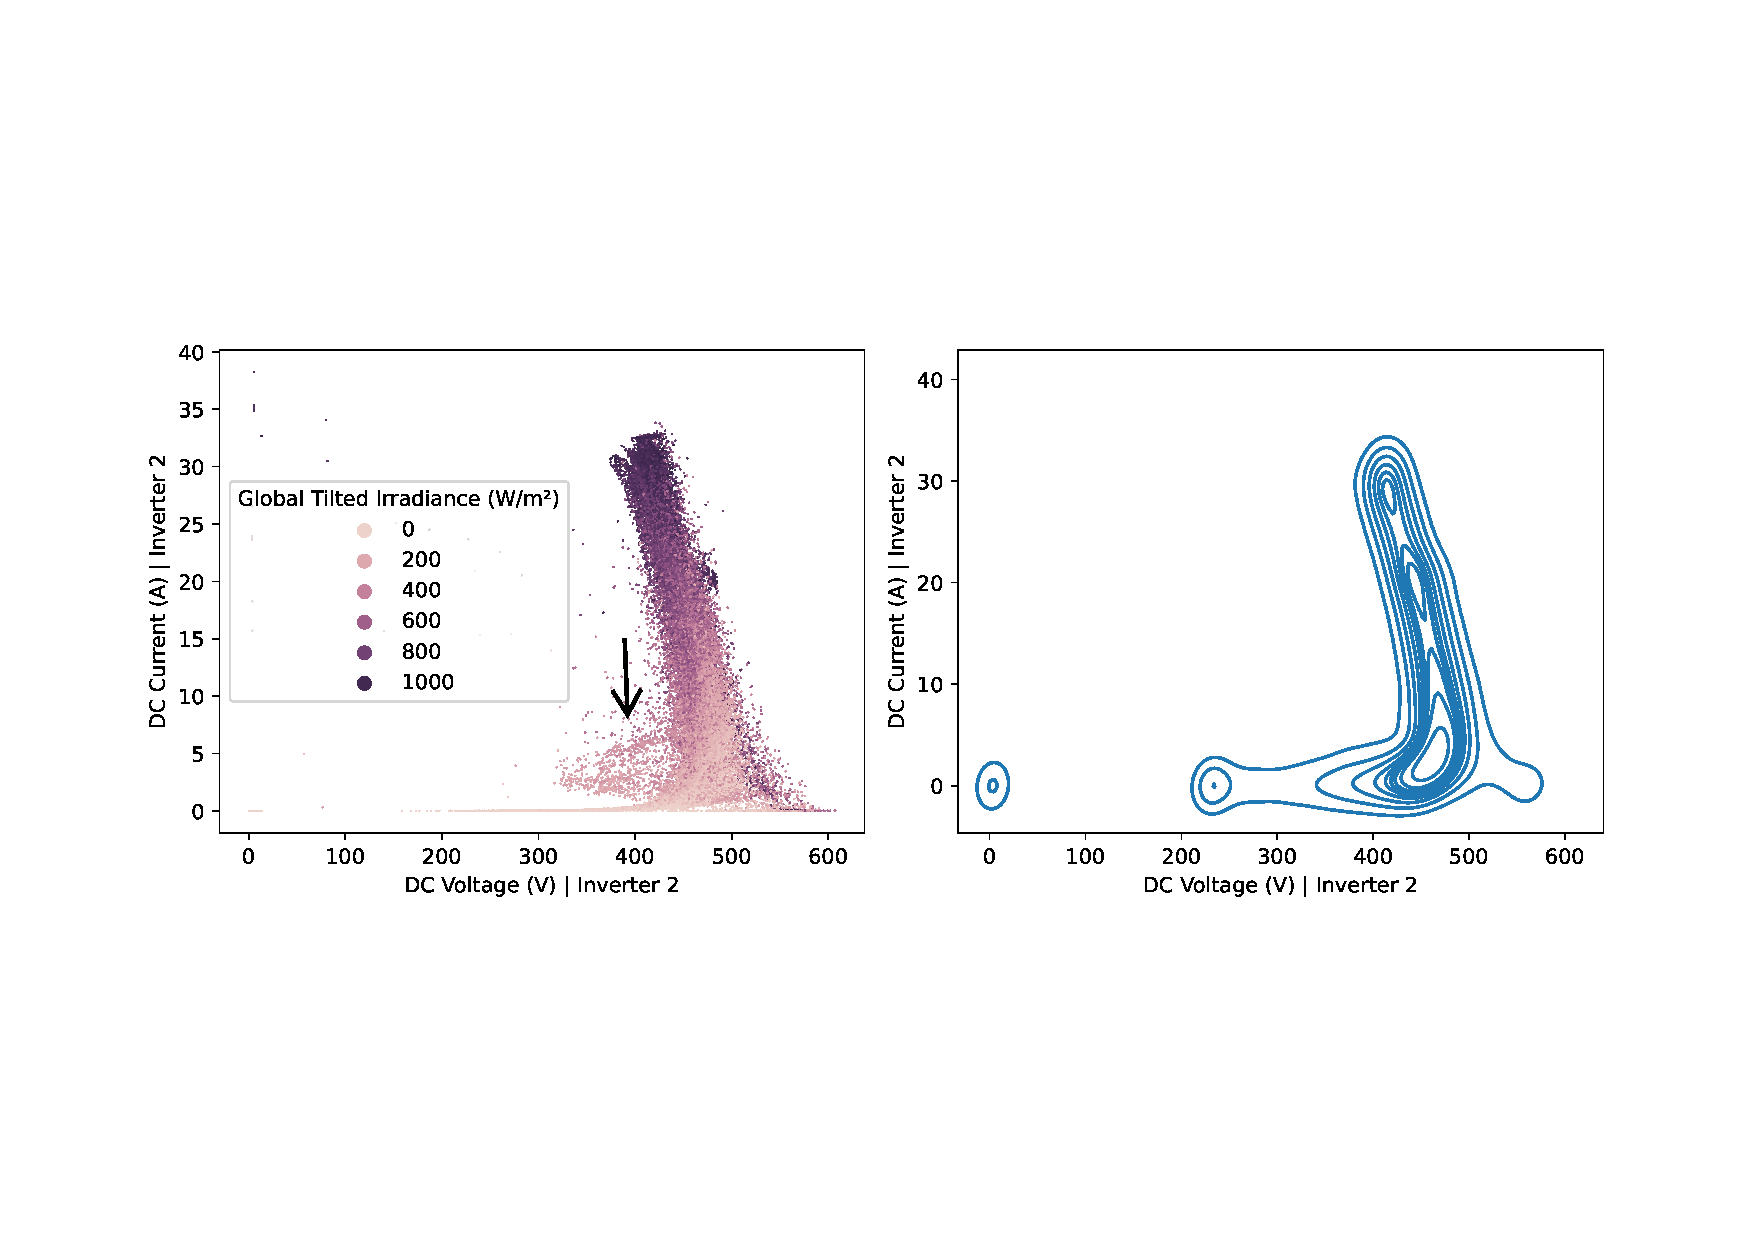
\includegraphics[width=\textwidth,trim={0 5.5cm 0cm 5.5cm},clip]{figures/chapter5/analysis/06_voltage_current_pairplot_kb_2_annotated.pdf}
    \caption{Pair plot of DC side voltage and current from inverter two (2020-2022), using scatter (left) and KDE (Kernel Density Estimation) (right).}
    \label{fig:eda_volt_curr_pair_kb_2}
\end{figure}

Regarding DC side voltage and current, figures \ref{fig:eda_volt_curr_pair_kb_1} and \ref{fig:eda_volt_curr_pair_kb_2} demonstrate the operating range of the inverter's MPPT. Both kickstart production at around 400 V and operate until close to 600 V. Between this range, the central column of samples represents voltage-current points relative to the knee of the strings' I-V curve (see figure \ref{fig:mpptcurve}), with irradiance generally increasing along its height. Some instances are outside this normal operation range (outliers), especially in the zone marked by the black arrow \textcircled{\raisebox{-0.9pt}{5}}\textcircled{\raisebox{-0.9pt}{6}}. These zones are critical because they represent inverter underperformance scenarios, which could be associated with some faults. It is denser in figure \ref{fig:eda_volt_curr_pair_kb_2}, meaning that inverter two has more underperforming situations; this was not completely clear from the previous analysis (figure \ref{fig:eda_power_kb_pair}). Appendix \ref{ap2:eda} presents the same charts, but for test data (figures \ref{fig:eda_voltage_current_test_1} and \ref{fig:eda_voltage_current_test_2}).

\subsubsection{Satellite} \label{subsubsec:eda_sat}

Irradiance should be the satellite variable most related to inverters' power. Therefore, we scatter both tilted and horizontal irradiance against AC power from inverters one and two.

\begin{figure}[h!]
    \centering
    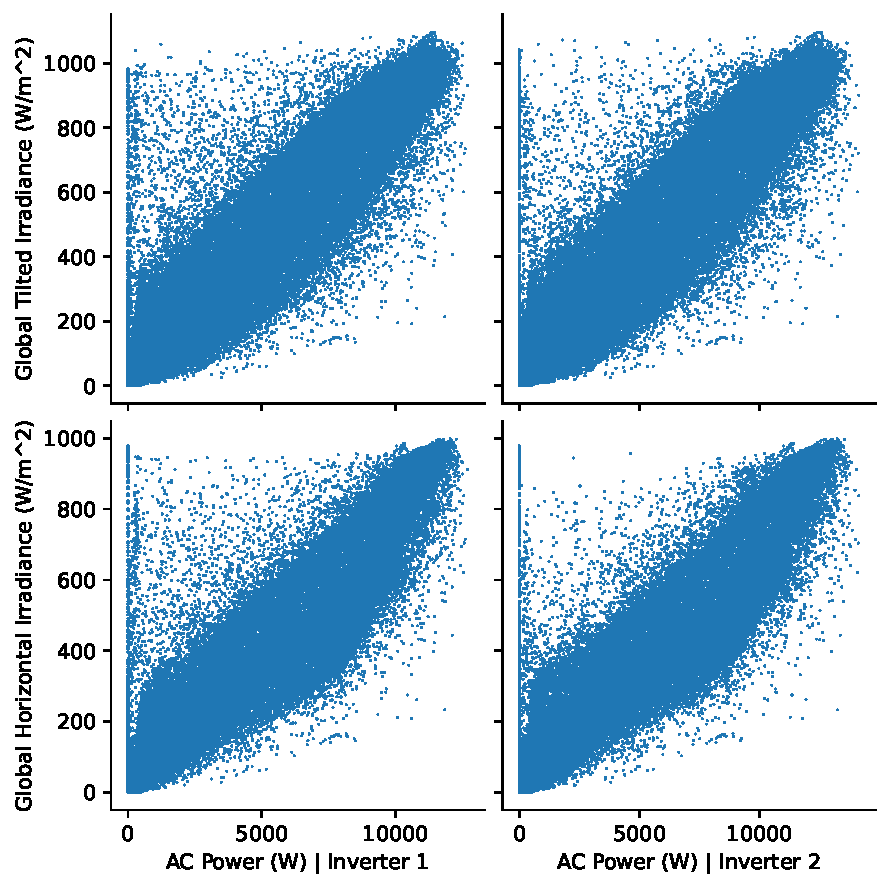
\includegraphics[width=0.8\textwidth]{figures/chapter5/analysis/08_power_irrad_pairplot_scatter_kb.pdf}
    \caption{Scatter pair plot of the AC power, tilted and horizontal global irradiance for both inverters (2020 to 2022).}
    \label{fig:eda_power_irrad_pair_kb}
\end{figure}

Figure \ref{fig:eda_power_irrad_pair_kb} shows the relationship between irradiance and AC power. We expected a positive correlation, and it exhibits such. However, the large radius around the central trend line demonstrates cycles around it that resemble some kind of hysteresis (especially with horizontal irradiance). By adding a color that displays the hour in each sample, we can affirm that these paths occur due to the fixed nature of the installed PV panels, having a characteristic curve from low to high irradiance in the sunrise and another from high to low during the sunset. Because they produce more with less sunlight in the morning, we can infer that they are oriented slightly towards the east.

Although most instances appear inside the sunrise-sunset paths, there are some outliers. The most notable are the ones of non-zero irradiance with zero production. Either error in satellite data or some anomaly in the inverters causes these odd scenarios, so we target them for cleaning the knowledge base.

Regarding the rest of the meteorological variables (cloud coverage and temperature), we deemed them unnecessary since they do not demonstrate a direct relationship with inverter behavior (see figure \ref{fig:eda_irrelevant_meteo}). We added KDE visualizations and plots for the test period in appendix \ref{ap2:eda}.

\section{Data Cleaning}

Now, we take our previous analysis and start the data-cleaning process. We used the Scikit-Learn Python Library and tried out some anomaly detection algorithms for outlier identification on our dataset: Robust Covariance \cite{Rousseeuw1999}, Isolation Forest \cite{Liu2008} \cite{Liu2012}, and Local Outlier Factor \cite{Breunig2000}. The code used for our plotting derived from an example made by Alexandre Gramfort, available on the Scikit-Learn website \cite{sklearn_example}.

\subsubsection{Power}

Based on the geographical proximity of the inverters, we have determined that the area around the trendline shown in figure \ref{fig:eda_power_kb} indicates standard operating points. Therefore, we must remove any samples deviating from this reference to clean the knowledge base.

\begin{figure}[h!]
    \centering
    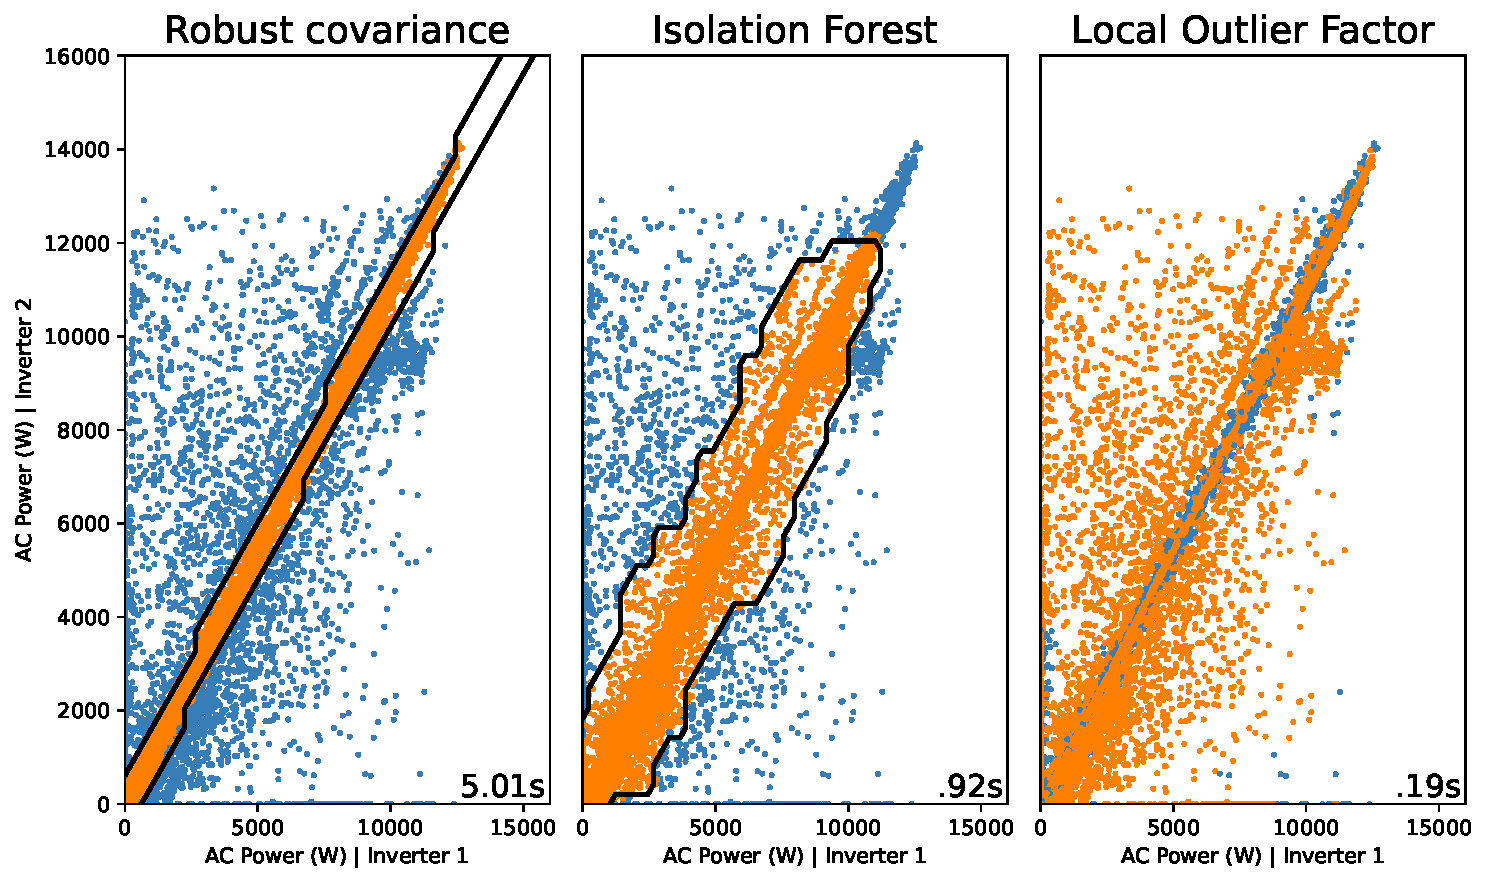
\includegraphics[width=\textwidth]{figures/chapter5/cleaning/20_cleaning_power.pdf}
    \caption{Inliers (orange), outliers (blue), and decision boundaries (black) using three different anomaly detection algorithms on the AC Power from both inverters.}
    \label{fig:clean_power}
\end{figure}

In Figure \ref{fig:clean_power}, we can see a visual representation of various anomaly detection algorithms' inliers, outliers, decision boundaries, and their computation time (bottom right). The algorithms are fine-tuned for approximately 14\% of outlier contamination. Based on the results, we determined that the Robust Covariance algorithm was the most effective since it extracted the region around the trend line without issues. We selected it to clean our knowledge base.

\subsubsection{Satellite}

In section \ref{subsubsec:eda_sat}, we discovered that the inverters follow a standard production pattern based on the irradiance and hour of the day. The specific area within the paths is considered the central region of standard operation. To clean up the data, we will remove all other instances.

\begin{figure}[h!]
    \centering
    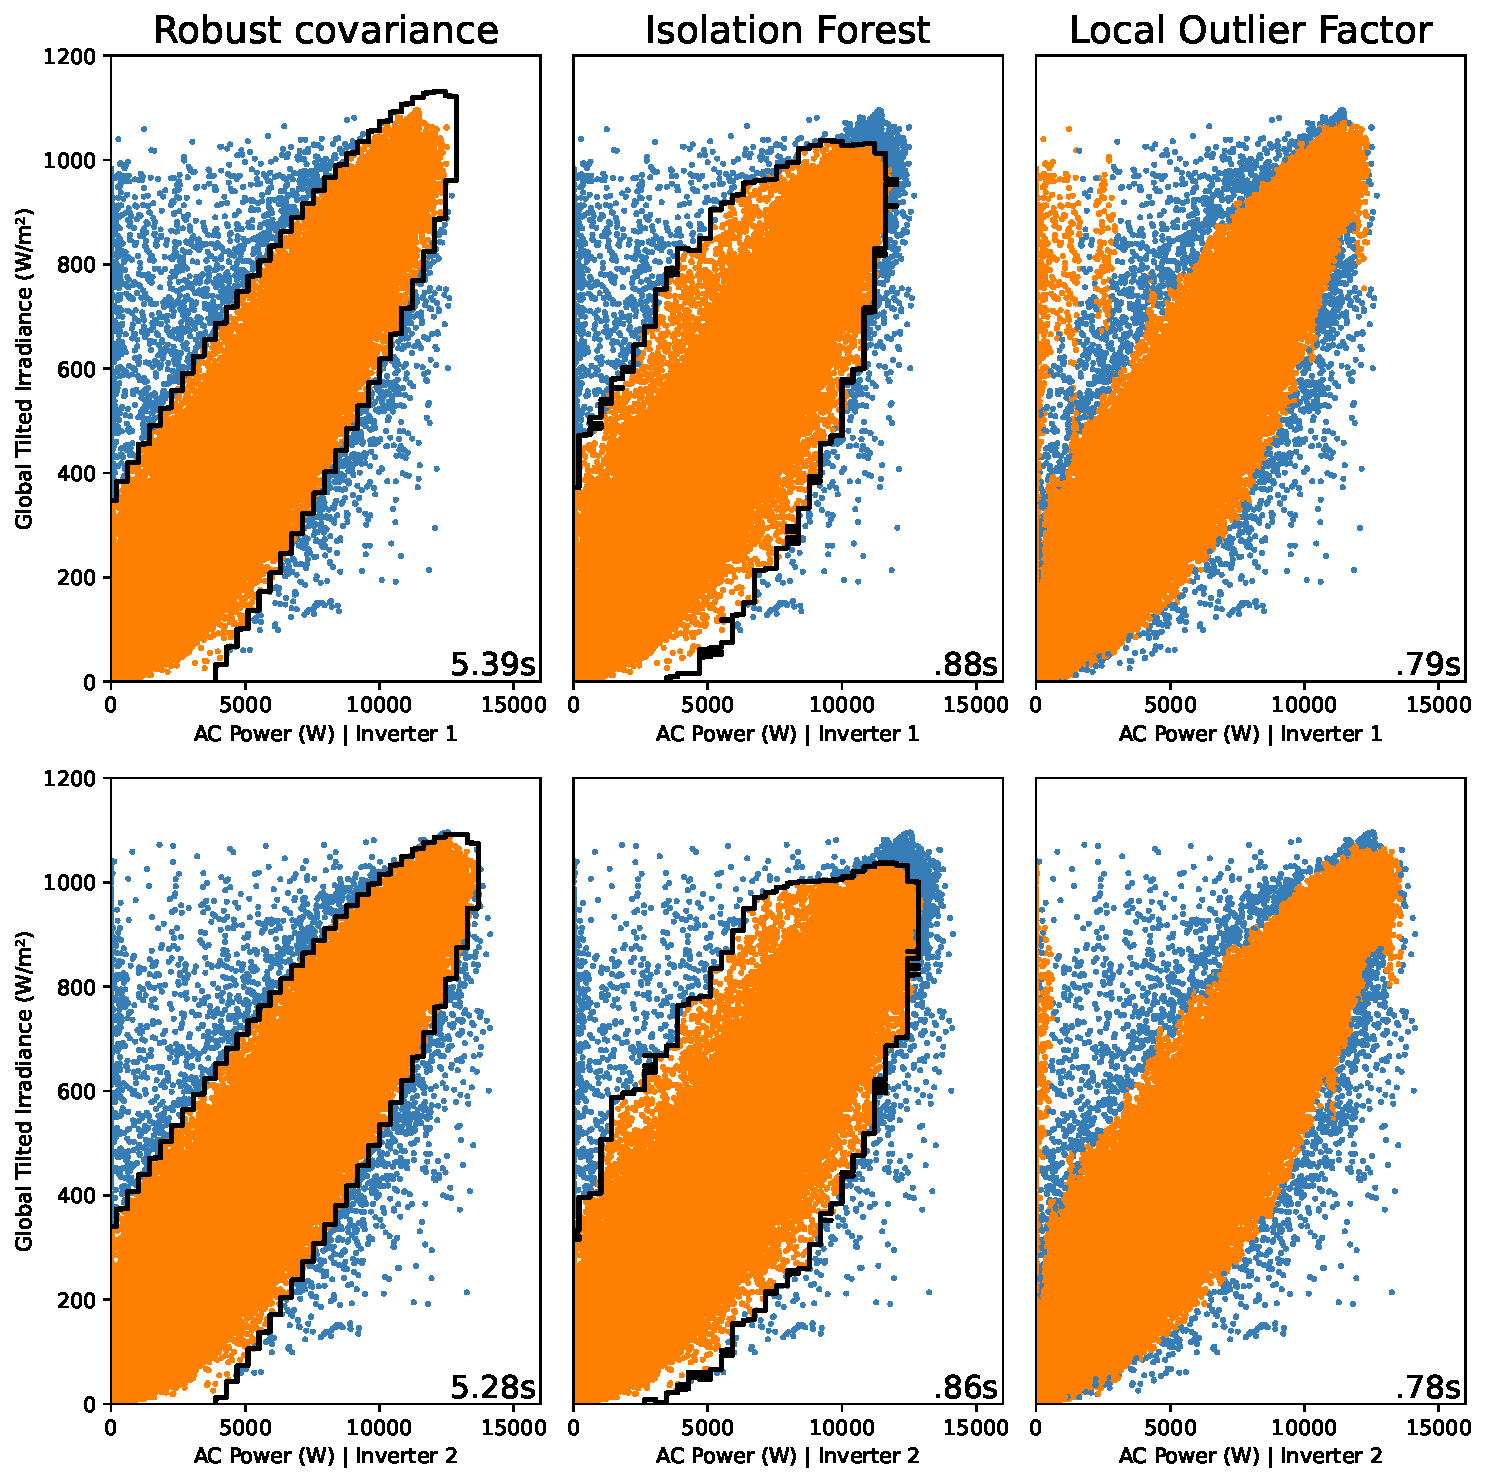
\includegraphics[width=\textwidth]{figures/chapter5/cleaning/21_cleaning_tilted_irrad.pdf}
    \caption{Inliers (orange), outliers (blue), and decision boundaries (black) using three different anomaly detection algorithms on the tilted irradiance and AC Power from both inverters.}
    \label{fig:clean_tilted_irrad}
\end{figure}

\begin{figure}[h!]
    \centering
    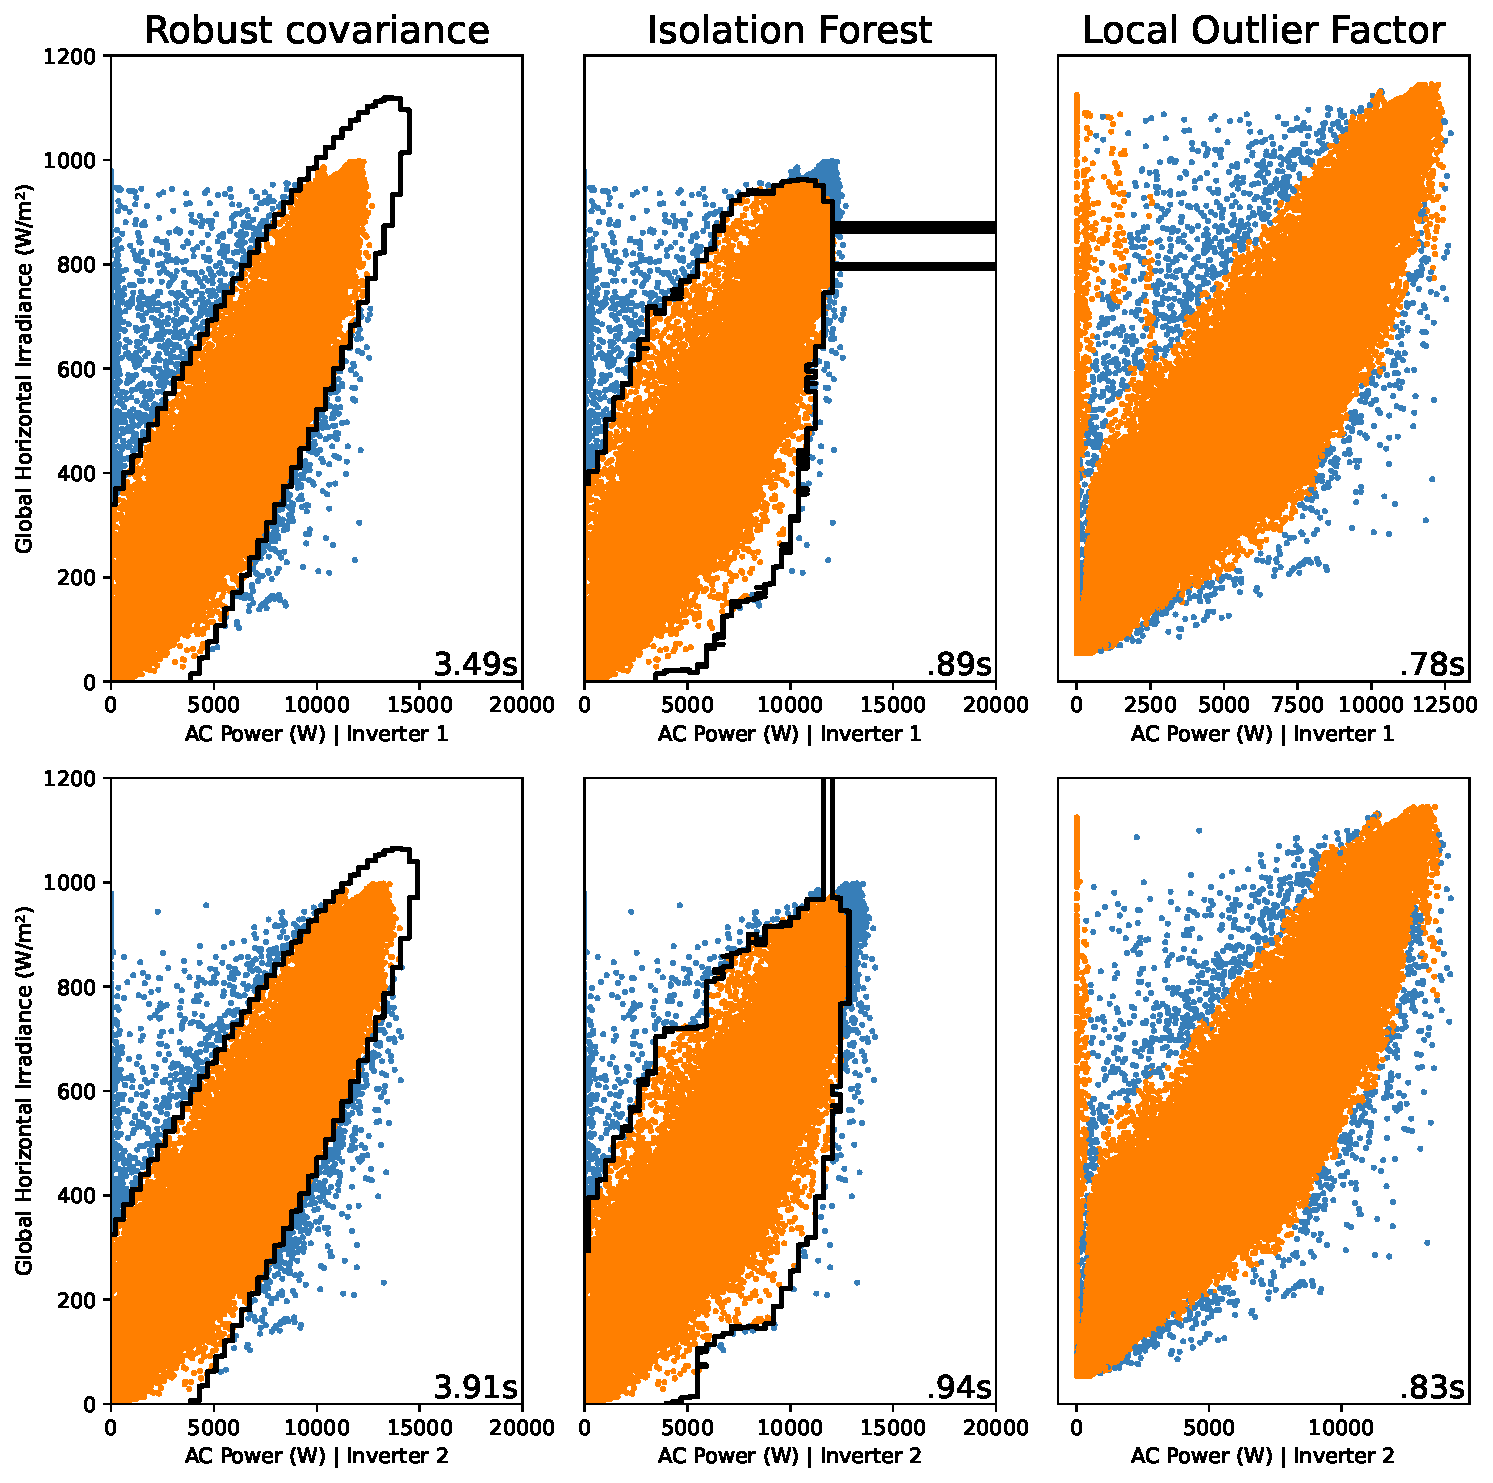
\includegraphics[width=\textwidth]{figures/chapter5/cleaning/22_cleaning_horizontal_irrad.pdf}
    \caption{Inliers (orange), outliers (blue), and decision boundaries (black) using three different anomaly detection algorithms on the horizontal irradiance and AC Power from both inverters.}
    \label{fig:clean_horizontal_irrad}
\end{figure}

Once again, figures \ref{fig:clean_tilted_irrad} and \ref{fig:clean_horizontal_irrad} demonstrate the effectiveness of the first algorithm, now for irradiance and power data. It is, once again, the chosen one for cleaning the knowledge base.

\subsubsection{Voltage and Current}

Cleaning voltage and current data were the most challenging thus far. The peculiar data distribution was an issue for all tested algorithms, and the isolation forest performed particularly poorly. We combined the Robust Covariance, and Local Outlier Factor results to obtain the best inlier-outlier separation. The aggregation performed was a logical "OR" considering the inliers.

\begin{figure}[h!]
    \centering
    \includegraphics[width=\textwidth]{figures/chapter5/cleaning/23_cleaning_volt_curr.pdf}
    \caption{Inliers (orange), outliers (blue), and decision boundaries (black) using two different anomaly detection algorithms and their combination on the DC side voltage and current from both inverters.}
    \label{fig:clean_volt_curr}
\end{figure}

The charts in figure \ref{fig:clean_volt_curr} illustrates how the algorithms have difficulty keeping up with the data's distribution and preserving the densely populated areas. Neither algorithm effectively identifies the outliers separately, but their combination proved much more effective.

\section{Photovoltaic Plugin}

According to the CellTAN formulation, cells cannot share their variables' data directly to maintain privacy. As a result, this limits plugins to work with only the information available in the cell they are running in. Therefore, inverter underperformance is the only situation considered for the PV plugin, based on the analysis from section \ref{subsubsec:eda_volt_curr}. Access to both the inverter's data and satellite data allows the owner to employ other algorithms that leverage this knowledge for better situational and fault discernment, but this falls back to the "classical" centralized algorithms, which is not the scope of this work.

We use the current and voltage samples resulting from the cleaning process to define the minimum operational boundary. Figure \ref{fig:pluginsteps} shows the proposed algorithm, which consists of the following steps:

\begin{itemize}
	\item Clean I-V data;
	\item Find the boundary points corresponding to the lowest voltage in the entire operating range;
	\item Fit a logarithmic function (\ref{eq:decayinglog}) to these points;
	\item Consider all points below the curve as situations of inverter underperformance.
\end{itemize}


Since data cleaning is already covered, we describe ways of determining the boundary points.
To begin, we establish bins for the current samples with a size of 1 A. Next, we examine each bin and determine the minimum voltage for that particular region via either the absolute minimum or a quantile. Once we have selected the reference minimum voltage, we record the bin's median current and minimum voltage as a boundary point.
After registering all boundary points, we use a curve-fitting algorithm to apply a decaying logarithmic function to them (equation \ref{eq:decayinglog}).

\begin{equation} \label{eq:decayinglog}
    V = a \times log(b \times I + c) + d \times I + e 
\end{equation}
where:
\begin{align*}
    V & : \text{Voltage (V)} \\
    I & : \text{Current (A)} \\
    a,b,c,d,e & : \text{Unknown constant parameters}
\end{align*}

\begin{figure}[h!]
    \centering
    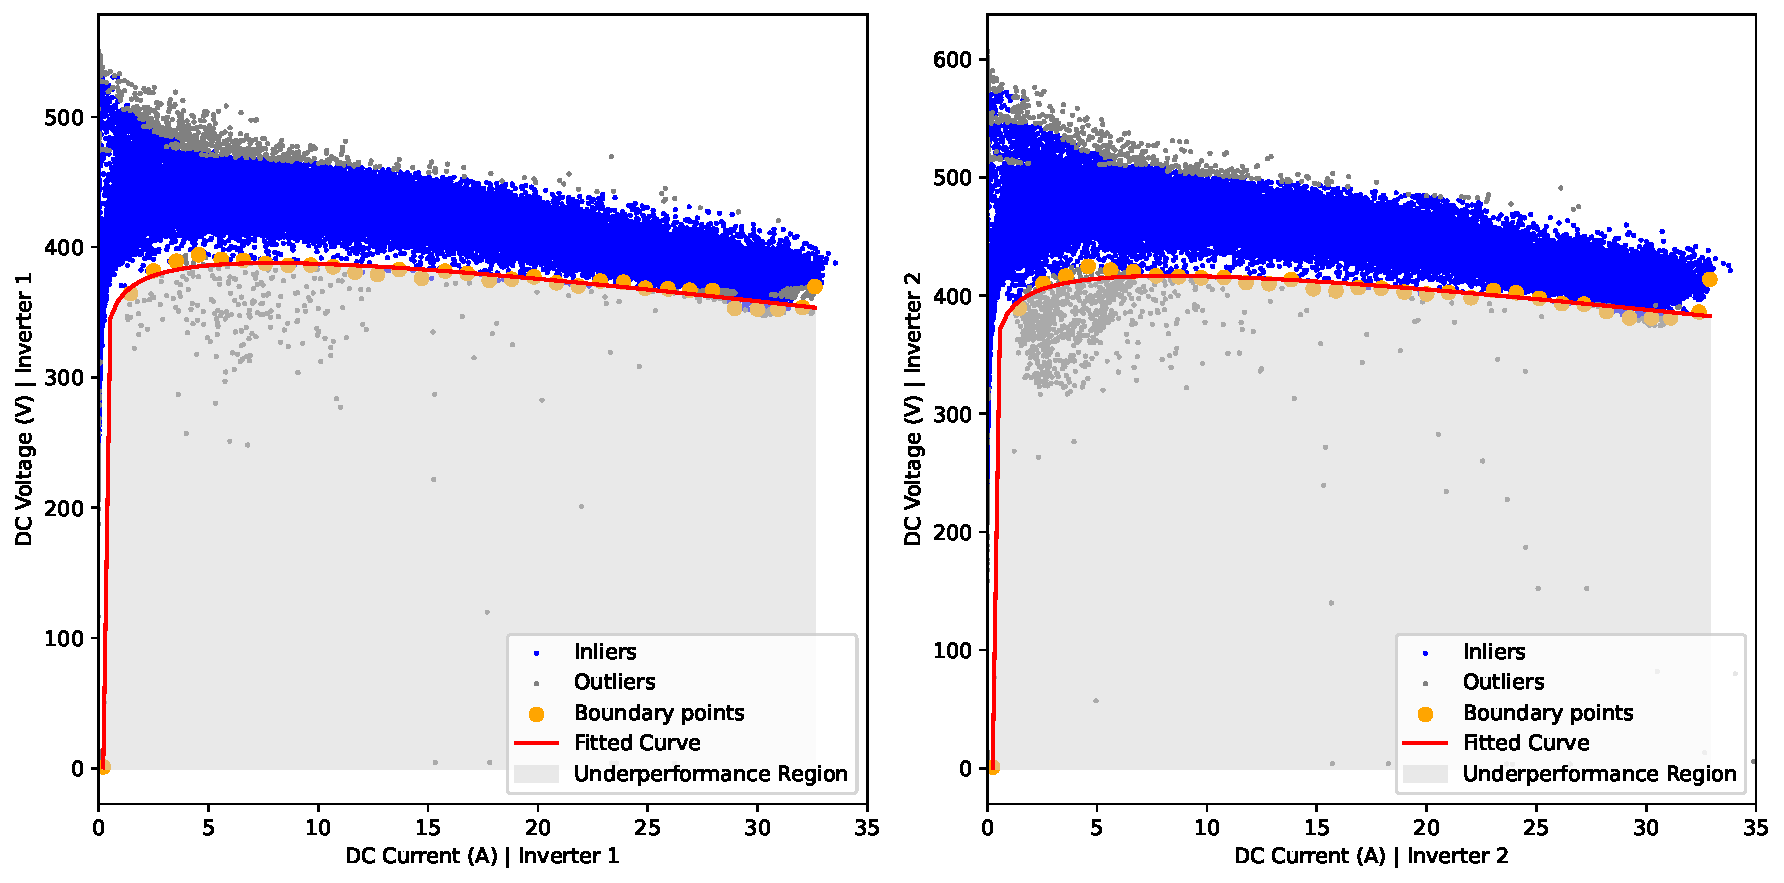
\includegraphics[width=\textwidth]{figures/chapter5/algorithm/30_boundary.pdf}
    \caption{Inverter underperformance region based on the lowest boundary of current-voltage inliers.}
    \label{fig:anomaly_decision_boundary}
\end{figure}

Figure \ref{fig:anomaly_decision_boundary} illustrates the outcome of using the described algorithm on our case study inverters. With the fitted curve's parameters, the PV plugin can analyze a new sample and determine if it falls under the underperformance category—whenever it does, the plugin flags that situation and reports back to the cell.
The fitted logarithmic curves are:

$$
    V_{inverter1} = 19.3 \times ln(169.2 \times I_{inverter1} - 35.2) - 2.8 \times I_{inverter1} + 276.1
$$

$$
    V_{inverter2} = 20.6 \times ln(148.3 \times I_{inverter2} - 35.6) - 2.9 \times I_{inverter2} + 299.5 
$$

\section{CellTAN Configuration}

The actual implementation of CellTAN requires a lot of time and resources to gather significant results. Therefore, we created a virtual scenario to simulate all test data and collect results quickly. The simulation involves cells using a fake in-memory implementation of some objects, such as its interface and repository. The interface is a cell dependency for communicating with other cells, and an in-memory implementation allows cells in the same host to share information directly. The repository is where the cell keeps its knowledge base and stores any persistent attributes (e.g. trust with neighbors). An in-memory repository eliminates the need to set up a database for experimentation.

To maintain time fidelity, which is crucial for this tool, we have the cells use a custom rolling timestamp generator that follows the time of each sample passed to the inputs. Effectively, all the mechanisms of the cell function without modification since their current time is always correct relative to the inputs. This timestamp method allows feeding inputs as fast as the cells perform their main process loop.

Selecting cell parameters can be difficult due to the complexness of variable uncertainties and thresholds (ref). However, we noticed that some parameter variations do not have a significant influence on making the CellTAN not function properly. We selected AC power, DC side current, and voltage for the inverters' inputs, considering 5\% uncertainty on all variables.

The complete cell configuration is available in appendix \ref{ap2:cellconfig}.

\section{Simulation and Results} \label{subsec:results}

\subsection{Artificial Scenario}

To validate the CellTAN core mechanisms with a controlled scenario, we simulate a network of just two cells (two inverters) with the same knowledge base (of inverter one). This way, we have a clean slate for introducing anomalies and watching the corresponding behavior. Translating to a real case, this would be most similar to two equal inverters with the same PV configuration installed in the same place.

\subsubsection{Simulation Without Anomalies}

The first validation is with an anomaly-free scenario. Here we simulate 72 samples of a clear day from 2023-03-02 06:30:00 to 2023-03-02 18:30:00.

\begin{figure}[h!]
    \centering
    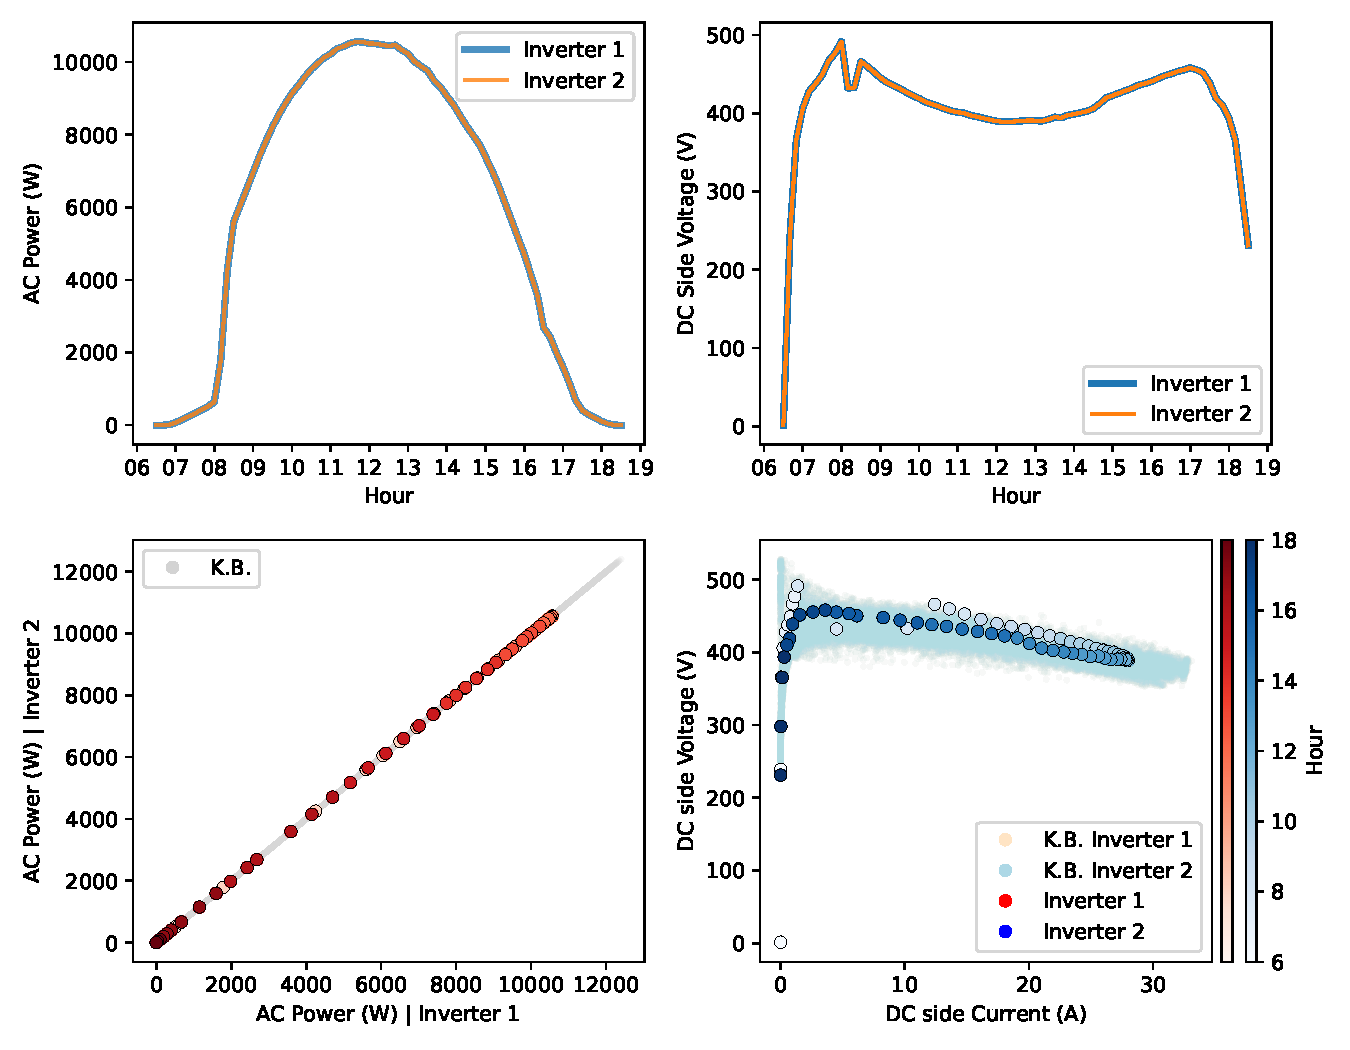
\includegraphics[width=\textwidth]{figures/chapter5/results/artificial/40_test_clone_01.pdf}
    \caption{Power, current and voltage profiles and scatter of simulation data for artificial scenario without anomalies.}
    \label{fig:artificial_01_piv}
\end{figure}

We will use figures like \ref{fig:artificial_01_piv} to present data that was used in the CellTAN to facilitate output interpretation. In it, K.B. refers to Knowledge Base, and the scatters allow us to better understand the region of the inputs against it.

\subsubsection{Simulation With Anomalies}

To assess all of the CellTAN's core mechanism, we simulate inverter mismatch and underperformance, which should influence the cells' trust and trigger the plugin into warning the situation.

\begin{figure}[h!]
    \centering
    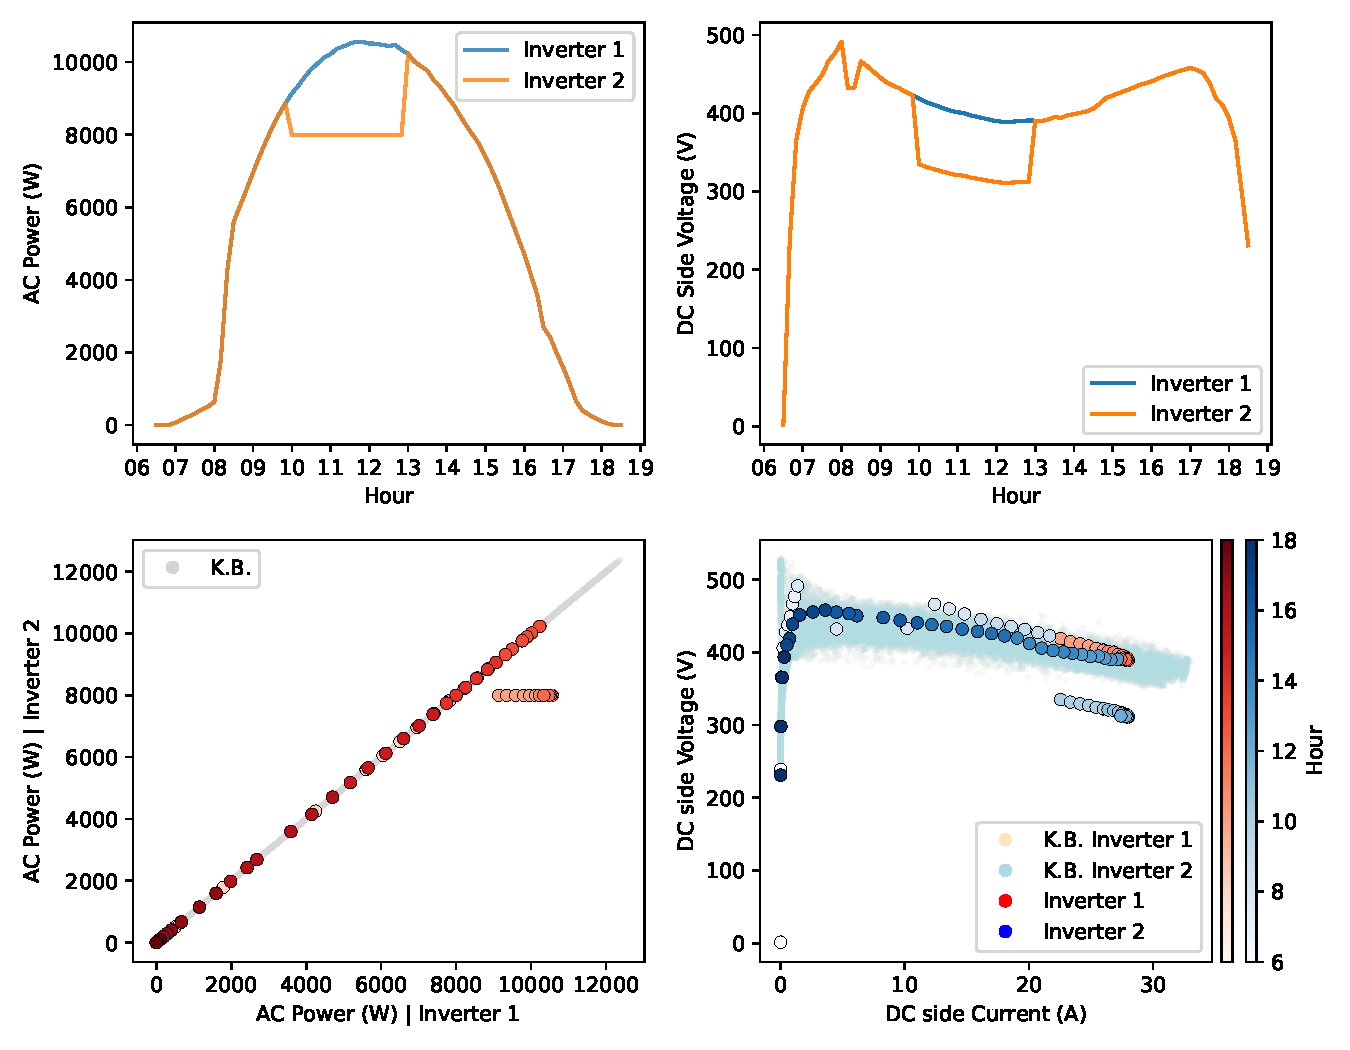
\includegraphics[width=\textwidth]{figures/chapter5/results/artificial/41_test_clone_02.pdf}
    \caption{Power, current and voltage profiles and scatter of simulation data for artificial scenario with anomalies.}
    \label{fig:artificial_02_piv}
\end{figure}

Figure \ref{fig:artificial_02_piv} shows the introduced anomalies from 9h to 12h. Regarding the scatter plots, we see that the AC Power strays into a region found during the analysis of the knowledge base (figure \ref{fig:eda_power_kb_pair} \textcircled{\raisebox{-0.9pt}{2}}), making it a relatively realistic setting. The voltage anomaly introduced is not as typical but still represents instances in the region mapped as underperformance in the PV plugin.


\subsection{Real Scenario}

Now, we use the test data from both inverters and satellite to run the CellTAN. By using 4 months' worth of data, it's possible to statistically evaluate the tool's outputs. However, it becomes challenging to select which specific portions to showcase in the following sections. Yet, this is also needed to understand real-time behavior, so the presented results will be hand-picked sections with relevancy.

\subsubsection{Typical Clear Sky Day}

\dots

\subsubsection{Typical Cloudy Day}

\dots

\subsubsection{Inverter-Inverter Mismatch}

\dots

\subsection{Inverters-Satellite Mismatch}

\dots

\subsection{Inverter Underperformance}

\dots

\subsection{Scaling Up}

\dots

% \begin{figure}[h!]
%     \centering
%     \includegraphics[width=\linewidth]{figures/chapter4/cell/celltan.pdf}
%     \caption{Ilustrative overview of a CellTAN.}
%     \label{fig:celltan}
% \end{figure}

% Figure \ref{fig:celltan} illustrates a simple CellTAN network overview. Regarding the \textbf{Hub}, one might infer (correctly) that a central component breaks the non-centralized paradigm. Nevertheless, it is present to solve some real-life implementation challenges and limitations, as will be further discussed in this chapter.

\chapter{Conclusion and Future Work} \label{chap:concl}

Proin sed justo eu sapien eleifend elementum. Pellentesque
habitant morbi tristique senectus et netus et malesuada fames ac
turpis egestas. Vivamus quam lacus, pharetra vel, aliquam vel,
volutpat sed, nisl. 

\section{Satisfação dos Objectivos}

Lorem ipsum dolor sit amet, consectetuer adipiscing elit. Etiam non
felis sed odio rutrum ultrices. Donec tempor dolor. Vivamus justo
neque, tempus id, ullamcorper in, pharetra non, tellus. Praesent eu
orci eu dolor congue gravida. Sed eu est. Donec pulvinar, lectus et
eleifend volutpat, diam sapien sollicitudin arcu, a sagittis libero
neque et dolor. Nam ligula. Cras tincidunt lectus quis nunc. Cras
tincidunt congue turpis. Nulla pede velit, sagittis a, faucibus vitae,
porttitor nec, ante. Nulla ut arcu. Cras eu augue at ipsum feugiat
hendrerit. Proin sed justo eu sapien eleifend elementum. Pellentesque
habitant morbi tristique senectus et netus et malesuada fames ac
turpis egestas. Vivamus quam lacus, pharetra vel, aliquam vel,
volutpat sed, nisl. 

Nullam erat est, vehicula id, tempor non, scelerisque at,
tellus. Pellentesque tincidunt, ante vehicula bibendum adipiscing,
lorem augue tempor felis, in dictum massa justo sed metus. Suspendisse
placerat, mi eget molestie sodales, tortor ante interdum dui, ac
sagittis est pede et lacus. Duis sapien. Nam ornare turpis et
magna. Etiam adipiscing adipiscing ipsum. Fusce sodales nisl a
arcu. Cras massa leo, vehicula facilisis, commodo a, molestie
faucibus, metus. Suspendisse potenti. Duis sagittis. Donec porta. Sed
urna. Maecenas eros. Vivamus erat ligula, pharetra sit amet, bibendum
et, fermentum sed, dolor. Nullam eleifend condimentum nibh. Integer
leo nibh, consequat eget, mollis et, sagittis ac, felis. Duis viverra
pede in pede. Phasellus molestie placerat leo. Praesent at tellus a
augue congue molestie. Proin sed justo eu sapien eleifend
elementum. Pellentesque habitant morbi tristique senectus et netus et
malesuada fames ac turpis egestas. 

\section{Future work}

Lorem ipsum dolor sit amet, consectetuer adipiscing elit. Aliquam
tempor tristique risus. Suspendisse potenti. Fusce id eros. In eu
enim. Praesent commodo leo. Nullam augue. Pellentesque tellus. Integer
pulvinar purus a dui convallis consectetuer. In adipiscing, orci vitae
lacinia semper, sapien elit posuere sem, ac euismod ipsum elit tempus
urna. Aliquam erat volutpat. Nullam suscipit augue sed
felis. Phasellus faucibus accumsan est. 

Aliquam felis justo, facilisis sit amet, bibendum ut, tempus ac,
dolor. Sed malesuada. Nunc non massa. In erat. Nulla
facilisi. Phasellus blandit, est in accumsan cursus, libero augue
elementum leo, vitae auctor mauris nisl ac tortor. Cras porttitor
ornare elit. Fusce at lorem. Sed lectus tortor, vestibulum id, varius
a, condimentum nec, lectus. Maecenas in nisi et magna pretium
aliquam. Pellentesque justo elit, feugiat nec, tincidunt a, dignissim
vel, ipsum. Sed nunc. Vestibulum ante ipsum primis in faucibus orci
luctus et ultrices posuere cubilia Curae; Aliquam tempus rhoncus
leo. Donec neque quam, cursus sit amet, ultricies varius, semper non,
pede. Donec porttitor. Sed aliquet feugiat elit.  

\vspace*{12mm}

Lorem ipsum dolor sit amet, consectetuer adipiscing elit. Phasellus
tellus pede, auctor ut, tincidunt a, consectetuer in, felis. Mauris
quis dolor et neque accumsan pellentesque. Donec dui magna,
scelerisque mattis, sagittis nec, porta quis, nulla. Vivamus quis
nisl. Etiam vitae nisl in diam vehicula viverra. Sed sollicitudin
scelerisque est. Nunc dapibus. Sed urna. Nulla gravida. Praesent
faucibus, risus ac lobortis dignissim, est tortor laoreet mauris,
dictum pellentesque nunc orci tincidunt tellus. Nullam pulvinar, leo
sed vestibulum euismod, ante ligula elementum pede, sit amet dapibus
lacus tortor ac nisl. Morbi libero. Integer sed dolor ac lectus
commodo iaculis. Donec ut odio.


%% comment next 2 commands if numbered appendices are not used
\appendix
\chapter{CellTAN Development}

\section{Statistical tests for measure of association} \label{ap1:stats}

\subsection{Pearson's chi squared test} \label{ap1:pearsonschi}

\begin{equation}
    \chi^2 = \sum_{i=1}^{k} \frac{(O_i - E_i)^2}{E_i}
\end{equation}
    
where:
\begin{align*}
\chi^2 & : \text{Chi-squared statistic} \\
O_i & : \text{Observed frequency for category } i \\
E_i & : \text{Expected frequency for category } i \\
k & : \text{Number of categories or cells in the data}
\end{align*}


\subsection{Fischer's exact test} \label{ap1:fischer}

\begin{equation}
    p = \frac{{\binom{a}{x} \binom{b}{y}}}{{\binom{N}{n}}}
\end{equation}

where:
\begin{align*}
    p & : \text{p-value of the test} \\
    a & : \text{Number of successes in group A} \\
    b & : \text{Number of successes in group B} \\
    x & : \text{Number of successes of interest in group A} \\
    y & : \text{Number of successes of interest in group B} \\
    N & : \text{Total number of observations} \\
    n & : \text{Number of observations in group A}
\end{align*}


\subsection{Odds ratio} \label{ap1:oddsratio}

\begin{equation}
OR = \frac{{a \cdot d}}{{b \cdot c}}
\end{equation}

where:
\begin{align*}
OR & : \text{Odds ratio} \\
a & : \text{Number of successes in group A} \\
b & : \text{Number of failures in group A} \\
c & : \text{Number of successes in group B} \\
d & : \text{Number of failures in group B}
\end{align*}

\subsection{Phi coefficient} \label{ap1:phi}

\begin{equation}
\phi = \sqrt{\frac{\chi^2}{N}}
\end{equation}

where:
\begin{align*}
\phi & : \text{Phi coefficient} \\
\chi^2 & : \text{Chi-squared statistic} \\
N & : \text{Total number of observations}
\end{align*}

\subsection{Contingency coefficient C} \label{ap1:contingencyc}

\begin{equation}
C = \sqrt{\frac{\chi^2}{N + \chi^2}}
\end{equation}

where:
\begin{align*}
C & : \text{Contigency coefficient} \\
\chi^2 & : \text{Chi-squared statistic} \\
N & : \text{Total number of observations}
\end{align*}


\subsection{Theil's U} \label{ap1:theilsu}

\begin{equation}
U(x|y) = \frac{H(x) - H(x|y)}{H(x)}
\end{equation}

Entropy of variable x:
\begin{equation}
H(x) = -\sum_{i=1}^{n} p(x_i) \log(p(x_i))
\end{equation}

Conditional entropy of variable x given variable y:
\begin{equation}
H(x|y) = -\sum_{i=1}^{n} \sum_{j=1}^{m} p(x_i, y_j) \log\left(\frac{p(x_i, y_j)}{p(y_j)}\right)
\end{equation}


\section{Technology stack} \label{ap1:techstack}

\begin{figure}[h!]
    \centering
    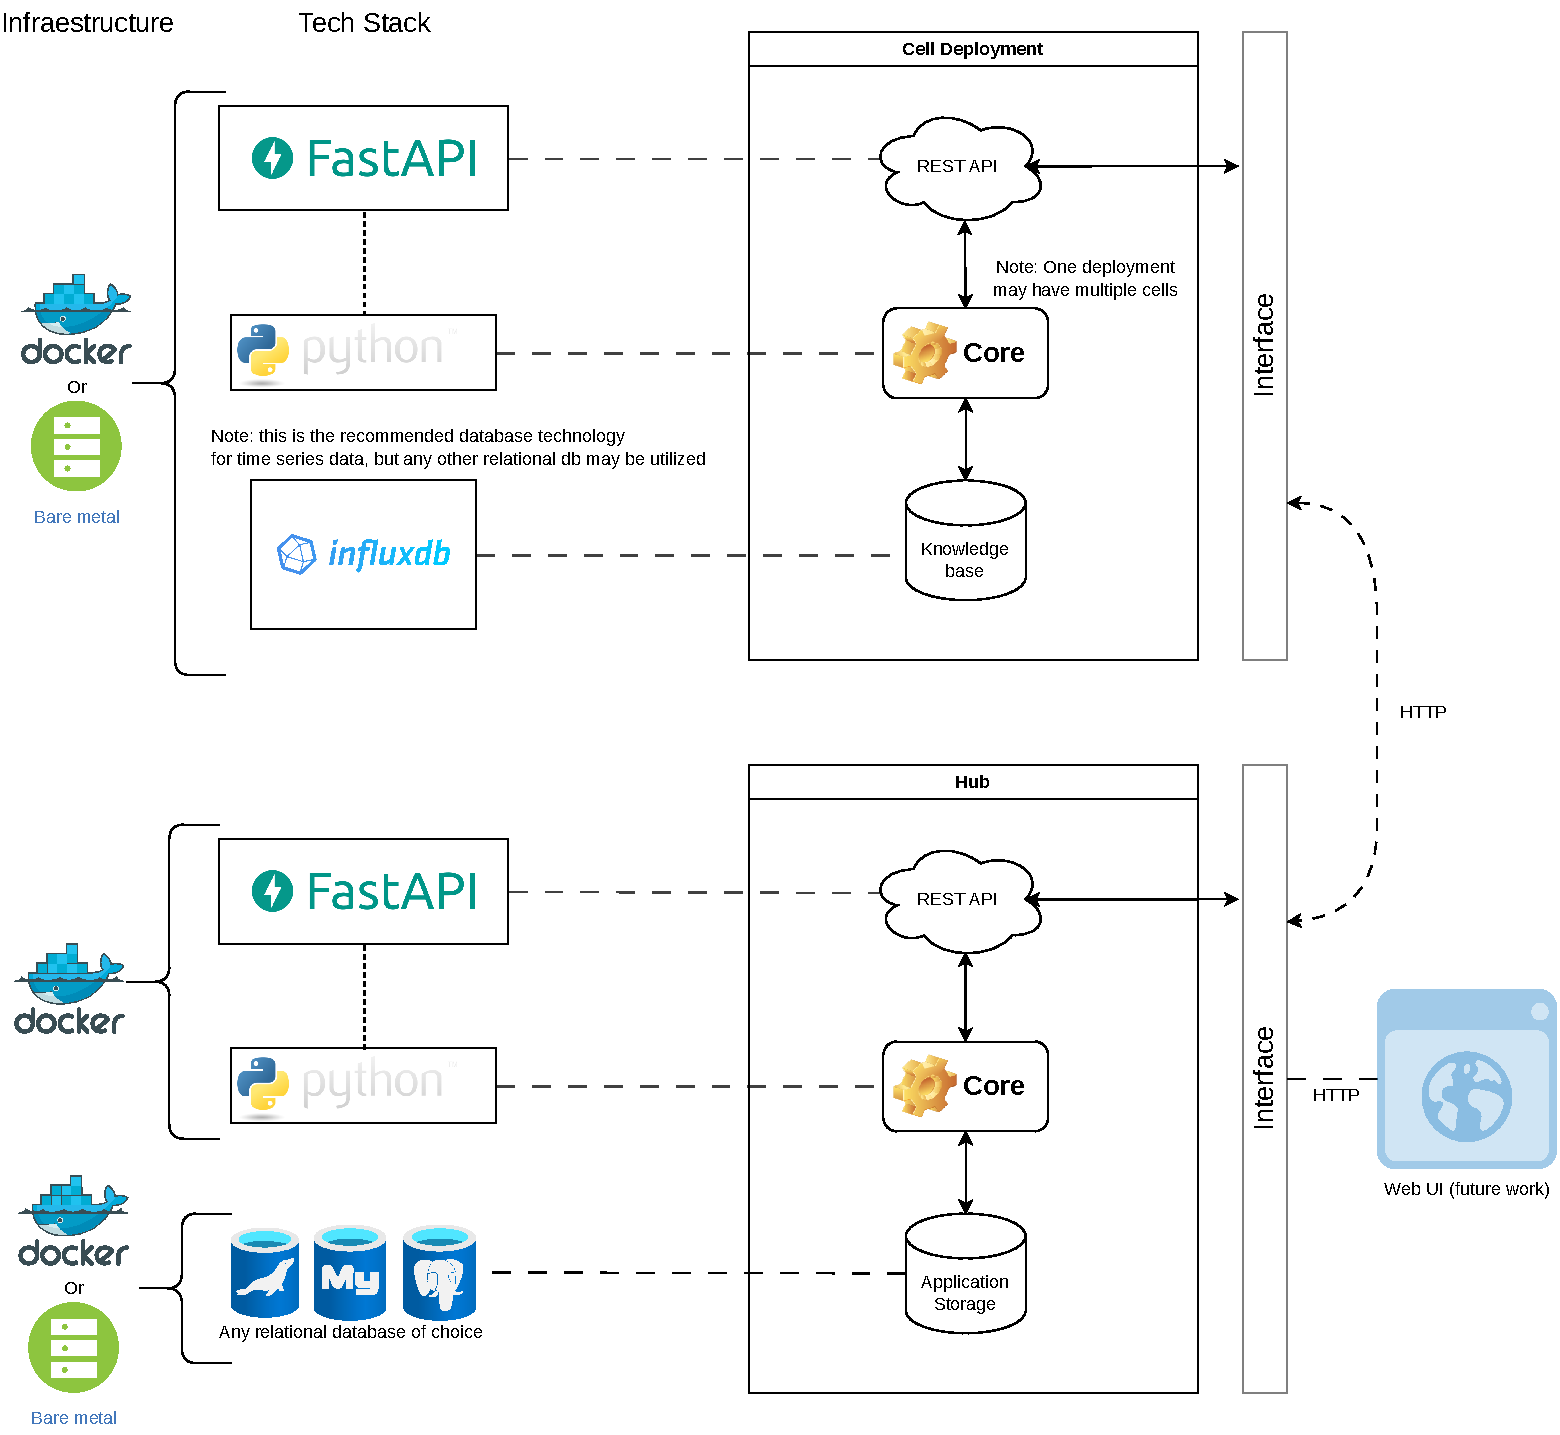
\includegraphics[width=\linewidth]{figures/appendix/a_development/techstack.pdf}
    \caption{Technology stack of the Cell and Hub of CellTAN.}
    \label{fig:techstack}
\end{figure}


\section{Cell configuration} \label{ap1:config}
 
% TODO overview da configuração da célula e ficheiro de configuração


%%----------------------------------------
%% Final materials
%%----------------------------------------

%% Bibliography
%% Comment the next command if BibTeX file not used
%% bibliography is in ``myrefs.bib''
\bibliography{myrefs}
\bibliographystyle{ieeetr}

%% Index
%% Uncomment next command if index is required
%% don't forget to run ``makeindex thesis'' command
%\PrintIndex

\end{document}
